% ============================================================
% APPENDIX -- detail moved out of the main text to keep sections within the house word targets
%   A  Method Definitions        sections/08a_method_definitions.tex (app:method-defs, sec:methods, sec:m-*)
%   B  Experimental Details      sections/08b_setup_details.tex      (app:setup-*, sec:setup-export,
%                                sec:setup-compute, sec:setup-deviations, tab:search, tab:compute)
%   C  Threats to Validity       sections/08c_validity.tex           (app:validity)
%   D  Additional Results        sections/08d_additional_results.tex (app:additional-results; figA1--A4,
%                                tab:dev-refusals-*, tab:capability-*, tab:teacher-forced-*; added 2026-11-06)
%   (D, cont.) Judging the First 256 Tokens   sections/08e_truncation256.tex (app:trunc256, tab:trunc256;
%                                added 2026-11-06; \subsection, so it continues Appendix D)
%   (D, cont.) Re-scoring the Released Exports on the Dev Set   sections/08f_dev_rescore.tex (app:dev-rescore,
%                                tab:dev-rescore, tab:dev-rescore-gemma2; added 2026-11-06; \subsection)
% The template placeholder that stood here (\section{Additional Methodological
% Detail} with \label{app:methods}) was replaced on 2026-11-05 by the three
% \input lines below. app:methods was never referenced; it is kept as an extra
% label on Appendix A (08a) so that any future \ref{app:methods} still resolves.
% The template's draft marker for appendix content was removed on 2026-11-05
% (todo pass): appendices A--D below supply the content, including
% 08d_additional_results.
% ============================================================
% =====================================================================
% APPENDIX: METHOD DEFINITIONS
% Moved on 2026-11-05 from the former main-text section "Refusal-Removal
% Methods" (sections/03_related_work.tex, draft v0 2026-11-04) when that
% section was rewritten as a house-style Related Work section
% (\label{sec:related}). Content is kept verbatim apart from cross-reference
% wording; every original \label is kept (sec:methods, sec:m-*).
% Table tab:methods stays in the Related Work section.
% Must be \input after \appendix (e.g. from sections/08_appendix.tex).
% =====================================================================
\section{Method Definitions}
\label{app:method-defs}
\label{sec:methods}
\label{app:methods}% former template placeholder label from 08_appendix.tex (never referenced; kept)

This appendix gives the notation, the update rule and the rationale of each
refusal-removal method reviewed in Section~\ref{sec:related}, together with
the strengths and weaknesses of each and the way it is instantiated in this
study.

\paragraph{Notation.}
A decoder-only transformer maintains a residual stream
$\mathbf{x}^{(\ell)} \in \mathbb{R}^{d}$ at each layer $\ell$. Each layer reads
from the stream and writes back to it through two matrices:
the attention output projection $W_O^{(\ell)}$ and the MLP down-projection
$W_{\mathrm{down}}^{(\ell)}$. Let $\mathcal{D}_{\mathrm{harm}}$ and
$\mathcal{D}_{\mathrm{safe}}$ be sets of harmful and harmless prompts, and let
$\boldsymbol{\mu}^{(\ell)}_{\mathrm{harm}}$ and
$\boldsymbol{\mu}^{(\ell)}_{\mathrm{safe}}$ be the mean residual activations at
the last prompt token over each set.

Methods are grouped by \emph{what they assume about refusal}: (i) it is a single
linear direction, (ii) it is a low-dimensional subspace or cone, (iii) it is
whatever transformation of each module's outputs separates harmful from
harmless inputs (no geometric assumption), or (iv) it is best located in a
different representation space altogether. Table~\ref{tab:methods}
(Section~\ref{sec:related}) summarises
the evaluated methods as instantiated in this study (\S\ref{sec:setup-methods}).

% ---------------------------------------------------------------------
\subsection{Single-direction methods}

\subsubsection{Classic abliteration (difference-in-means)}
\label{sec:m-dim}
\textbf{Mechanism.} Compute the refusal direction
$\hat{\mathbf{r}}^{(\ell)} =
\mathrm{normalize}(\boldsymbol{\mu}^{(\ell)}_{\mathrm{harm}} -
\boldsymbol{\mu}^{(\ell)}_{\mathrm{safe}})$, pick one layer's direction
$\hat{\mathbf{r}}$, and orthogonalise every matrix that writes to the residual
stream against it:
$W \leftarrow W - \lambda\,\hat{\mathbf{r}}\hat{\mathbf{r}}^{\top} W$
\cite{arditi2024refusal}. With $\lambda=1$ the model can no longer write any
component along $\hat{\mathbf{r}}$.

\textbf{Why it works.} Under the linear representation hypothesis
\cite{park2024linear}, high-level features correspond to directions.
Arditi et al.~\cite{arditi2024refusal} showed causally that adding $\hat{\mathbf{r}}$
induces refusal on harmless prompts and ablating it suppresses refusal on
harmful ones, across 13 chat models. Because the edit is a rank-one projection,
most of the weight matrix is untouched.

\textbf{Why it exists.} It turned an interpretability finding into a
practical, training-free procedure that needs only forward passes on a few
hundred prompts \cite{labonne2024abliteration,failspy_abliterator}.

\textbf{Pros.} Simple, fast (minutes), interpretable, rank-one, few
hyperparameters (layer, strength).
\textbf{Cons.} Assumes refusal is one-dimensional; the direction also carries
part of the harmless mean, so removing it damages unrelated behaviour (refusal
is better described as an affine function whose offset plain ablation ignores;
on a recurrent RWKV model plain ablation produced nonsense where affine concept
editing stayed coherent \cite{marshall2024refusal}); changing row norms shifts
activation scales; quality depends heavily on the chosen layer and strength,
which are usually set by hand (in an earlier cross-tool comparison, GSM8K
accuracy changed by between $+1.51$ and $-18.81$ percentage points
\cite{young2025comparative}). DECCP, ErisForge and
FailSpy's tool are implementations of this recipe with different layer-selection
heuristics. In this study diff-in-means runs inside Heretic with the same
automated search over direction, strength and layer profile as MPOA
(``Heretic-tuned DiM'', \S\ref{sec:setup-methods}).

\subsubsection{Projected and magnitude-preserving abliteration (MPOA)}
\label{sec:m-mpoa}
\textbf{Mechanism.} Two refinements of \S\ref{sec:m-dim}.
(1) \emph{Projection}: remove from $\hat{\mathbf{r}}$ its component along the
normalised harmless mean, so that only the part of the refusal direction
orthogonal to ordinary activations is ablated \cite{lai2024projected}.
(2) \emph{Magnitude preservation}: row-normalise $W$, apply the ablation, then
restore each row's original norm \cite{lai2025mpoa}.
Heretic adds a search over a per-layer weight kernel (peak strength, peak
position, minimum strength, falloff distance) for attention and MLP separately,
global versus per-layer directions, and a fractional direction index
interpolated between layers, all tuned by multivariate TPE
\cite{akiba2019optuna,heretic2025}. The edit is stored as a low-rank LoRA
adapter \cite{hu2022lora}.

\textbf{Why it works.} Projection reduces collateral damage: the part of
$\hat{\mathbf{r}}$ shared with harmless activations is exactly what is
needed for normal behaviour. Norm preservation keeps downstream layer norms and
activation magnitudes in the range the model was trained on, so edits
change \emph{direction} rather than \emph{scale}.

\textbf{Why it exists.} Plain abliteration measurably degraded capability
(for example GSM8K drops of several points in an earlier comparison
\cite{young2025comparative}); these refinements recover much of that loss.

\textbf{Pros.} Better capability retention at the same refusal rate;
automated hyperparameter search removes manual tuning.
\textbf{Cons.} Still assumes a single direction per layer; norm preservation is
only approximate when stored as a low-rank adapter; the search adds many
evaluation passes (one per trial).

\subsubsection{Null-space-constrained abliteration (jwest33)}
\label{sec:m-null}
\textbf{Mechanism.} Compute a projected, norm-rescaled diff-in-means edit
$\Delta W$ as above, then restrict it to the null space of activations on a
set of \emph{preservation} prompts: with $V$ the top singular vectors of
those activations, apply $\Delta W (I - V V^{\top})$
(the AlphaEdit constraint \cite{fang2025alphaedit}). Optional Gaussian layer
weighting spreads the edit around a chosen depth.

\textbf{Why it works.} If an input lies in the span of $V$, the constrained
edit has no effect on it, so behaviour on preserved inputs is guaranteed
unchanged to first order; the edit can only act on directions that harmless
inputs do not use.

\textbf{Why it exists.} It brings guarantees from knowledge editing
\cite{meng2022locating,fang2025alphaedit} to refusal removal, as an
alternative to tuning strength against a KL budget.

\textbf{Pros.} Principled protection of chosen behaviour; single pass, no
search.
\textbf{Cons.} If harmful and harmless activations share directions (likely in
newer models), the constraint also blocks the refusal edit; the rank ratio is a
new hyperparameter; dense models only in the current implementation. It is not
evaluated in this study (\S\ref{sec:m-not}).

% ---------------------------------------------------------------------
\subsection{Multi-direction and subspace methods}

\subsubsection{SVD multi-direction (Gabliteration, OBLITERATUS presets)}
\label{sec:m-svd}
\textbf{Mechanism.} Instead of the mean difference, take the top-$k$ singular
vectors of the matrix of per-prompt differences between harmful and harmless
activations, and project all $k$ out, typically with ridge regularisation and
selected layers \cite{gabliteration2024}. OBLITERATUS packages this
(``advanced'', 4 directions), whitened and iterative variants (``aggressive''),
frequency-band weighting of layers via a DCT (``spectral cascade''), and a
re-implementation of gradient-refined directions (``rdo'') in one toolkit.

\textbf{Why it works.} When refusal is spread over several correlated
directions, one mean difference captures only the dominant one; the remaining
components can re-trigger refusal. Removing a subspace closes those
alternative routes.

\textbf{Why it exists.} Single-direction ablation leaves residual refusals on
some prompt categories and some models; multi-direction methods target that
residual.

\textbf{Pros.} Removes more refusal on models where one direction is
insufficient; still closed-form and fast.
\textbf{Cons.} Every extra direction removed is extra capacity destroyed;
choosing $k$ trades refusal against damage; several presets are heuristic
combinations without a clear theoretical justification. The OBLITERATUS
v0.1.4 presets \texttt{advanced} and \texttt{spectral\_cascade}, together with
\texttt{basic}, are not evaluated in this study; they were run on
Qwen2.5-7B-Instruct and scored with this study's harness in the companion
paper \cite{young2026paper30}. Version 0.1.4 lists a \texttt{som} preset but
does not ship its direction module and does not run on Qwen3.5-4B
(Appendix~\ref{app:setup-methods}).
% src (2026-11-06, author decision: OBLITERATUS reported in paper 30 only): results/bench-4090/qwen2.5-7b__obliteratus-{basic,advanced,spectral_cascade}/push_manifest.json;
% scripts/run_external_small.sh (header NOTE: som extractor obliteratus.analysis.som_directions not shipped; v0.1.4 fails closed on every Qwen3.5); ../paper30/v3_2611/analysis/RESULTS.md

\subsubsection{Refusal cones (RDO)}
\label{sec:m-rdo}
\textbf{Mechanism.} Learn refusal directions by gradient descent on an
objective that requires ablation to remove refusal and addition to induce it,
while keeping other behaviour fixed; multiple such directions form a
polyhedral \emph{concept cone} \cite{wollschlager2025geometry}.

\textbf{Why it works / exists.} It showed that refusal is not a single
direction but a multi-dimensional cone of causally relevant, representationally
independent directions, and that directions found by optimisation outperform
diff-in-means.
\textbf{Pros.} Directly targets the causal effect rather than a statistical
proxy. \textbf{Cons.} Requires gradients and more compute. It is not evaluated
in this study (\S\ref{sec:m-not}).

\subsubsection{Self-organising-map directions (SOM)}
\label{sec:m-som}
\textbf{Mechanism.} Fit a small self-organising map (e.g.\ $4\times4$) to the
harmful activations at each layer, take $k$ map neurons as prototypes of
distinct ``kinds'' of harmful input, and use each prototype minus the harmless
mean as a refusal direction; ablate all $k$, each with its own strength
\cite{piras2025som}. The proof-of-concept Heretic integration (PR~\#196)
tunes the per-direction strengths with TPE.

\textbf{Why it works.} Different harm categories (weapons, self-harm, cyber,
\ldots) may trigger refusal through different directions; a single mean
averages them and represents none well. The SOM finds the clusters
without labels. Piras et al.~\cite{piras2025som} show diff-in-means is a special case.

\textbf{Pros.} Strong reported results (3/100 refusals at KL $\approx 0.1$ on
gpt-oss-20b, PR~\#196); principled multi-direction choice.
\textbf{Cons.} More hyperparameters (map size, $k$, per-direction strengths)
make TPE converge slowly; the PoC's top-$k$ selection counts winners over the
map's own weights instead of the data. In this study SOM is ported to
Heretic~2.0 as a modifier (``Heretic-tuned SOM'') that ranks neurons by wins
over the harmful residuals, orthonormalises the $k$ directions and replaces the
per-direction strengths with one searched decay; these and the other deviations
from Piras et al.~\cite{piras2025som} are listed in \S\ref{sec:setup-deviations}.

% ---------------------------------------------------------------------
\subsection{Optimisation-based methods}

\subsubsection{Arbitrary-Rank Ablation (ARA)}
\label{sec:m-ara}
\textbf{Mechanism.} ARA makes no assumption about the geometry of refusal
\cite{weidmann2026ara}. For each targeted linear module $W$ in a layer range
(in Heretic, the attention output projection and the MLP down-projection), it
records the module's inputs $X$ and outputs $Y = XW^{\top}$ on harmless
($g$) and harmful ($b$) prompts, then learns a low-rank update
$\Delta W = BA$ (rank 50 by default) minimising
\begin{equation}
\label{eq:ara-objective}
\mathcal{L} = w_p\,\big\|\tilde{Y}_g - Y_g\big\|^2
 + w_s\Big[\,d_k(\tilde{Y}_b, Y_g) - w_o\, d_k(\tilde{Y}_b, Y_b)\Big],
\end{equation}
where $\tilde{Y}$ is the output of $W+BA$ with each row rescaled to the norm of
the corresponding row of $W$, and $d_k(\cdot,\cdot)$ is the mean distance to the
$k$ nearest neighbours. The rescaling enters only the objective; the exported
adapter $BA$ is not renormalised (\S\ref{sec:setup-methods}).
The three terms keep harmless outputs fixed, pull harmful outputs toward
harmless ones, and push them away from where they were (``overcorrection'').
Each module is solved independently with L-BFGS; Heretic's TPE searches the
layer range, the three weights and $k$.

\textbf{Why it works.} Rather than guessing the shape of the refusal
representation, ARA directly asks each module to make harmful inputs produce
the outputs harmless inputs produce. Any refusal mechanism that a module's
output carries, whether linear, multi-directional or non-linear across
prompts, is in scope, up to the adapter's rank. The objective is close to
convex and starts at its optimum for the preservation term, so L-BFGS
converges in a few iterations.

\textbf{Why it exists.} Its author reports that directional ablation
increasingly fails on recent models, and that ARA reaches lower refusal at
lower KL on gpt-oss-20b than any directional result \cite{weidmann2026ara}.

\textbf{Pros.} No geometric assumption; fewer search parameters than
per-component directional kernels; memory similar to abliteration because
modules are solved one at a time.
\textbf{Cons.} Slower per trial; rank-50 adapters per module are larger
artefacts; the nearest-neighbour objective depends on the prompt sets, so it
may overfit them; no published analysis yet (preprint forthcoming).

% ---------------------------------------------------------------------
\subsection{Methods in other representation spaces}

\subsubsection{Jacobian-space (J-space) ablation}
\label{sec:m-jspace}
\textbf{Mechanism.} Using a Jacobian lens, map each layer's activations into a
``workspace'' where features are read out by the model's later computation;
compute the refusal direction there and pull it back to the residual stream
through the layer Jacobian, $\mathbf{d}_\ell = J_\ell^{\top}(\cdot)$; ablate it
with a forward hook rather than a weight edit
\cite{sekinal2026jspace}.

\textbf{Why it exists.} To localise the part of the refusal signal the model
actually uses downstream, rather than everything correlated with harmfulness.
\textbf{Pros.} Very targeted (small distribution shift).
\textbf{Cons.} By its authors' own measurements removes little refusal
(AdvBench refusal 0.78 versus 0.06 for diff-in-means on Qwen3.5-4B); the
reference code is hook-based, so not directly an exportable model, and is a
single-model implementation. In this study the J-space directions are instead
baked into the weights with Heretic's directional-ablation edit and search
(full row normalisation, no harmless-mean projection), which yields an
exportable model (\S\ref{sec:setup-methods}); the reference forward hook is
planned as a further condition. Because, among the candidate models,
instruction-tuned Jacobian lenses (\texttt{neuronpedia/jacobian-lens}) exist
only for the two small-pair models, J-space is run on the small pair only.

% ---------------------------------------------------------------------
\subsection{Methods not evaluated}
\label{sec:m-not}
Null-space-constrained abliteration (\S\ref{sec:m-null}) and refusal cones
(\S\ref{sec:m-rdo}) are described above for completeness but are not part of
the final design. A code audit before the main runs found that the available
null-space implementation (\texttt{jwest33/abliterator}) applies the
constraint on the output side, where it gives no preservation guarantee, and
edits square attention output projections, as in Qwen2.5-32B, OLMo-2-32B,
Olmo-3.1-32B and Mistral-Small-2409, in the wrong space; the revised
plan therefore dropped it. The only RDO implementation considered, the
\texttt{rdo} preset of OBLITERATUS, is a probe-based proxy rather than the
gradient-based optimisation of Wollschl\"ager et
al.~\cite{wollschlager2025geometry}, and it is not among the OBLITERATUS
presets evaluated in the companion paper \cite{young2026paper30}.
% src (2026-11-05 todo pass): notes/EXECUTION_PLAN_v2.md (finding 9: "jwest33 square-o_proj bug"; Design: no null-space condition; small-pair OBLITERATUS presets basic/advanced/spectral_cascade/som); notes/methods_survey_other_tools.md (jwest33 null-space constraint; OBLITERATUS presets incl. rdo); notes/session_logs/transcripts_redacted/b7a10890-24c5-4939-ba96-da845ba9da41.jsonl (code-audit report, line 4489: jwest33 "AlphaEdit-style null-space constraint, but it is applied on the output side, so it gives no preservation guarantee. Has the square o_proj bug"; "abliterate.py:2085,2157 and null_space.py:314 test the input dimension first. A square o_proj (Qwen2.5-32B, OLMo-2-32B, Olmo-3.1-32B, Mistral-Small-2409) is therefore ablated in the wrong space"; "Its rdo is a probe-proxy, not Wollschlaeger's RDO"; line 7173: null-space "dropped because its tool was buggy"). No note gives a separate, explicit reason for leaving the OBLITERATUS rdo preset out of the plan. (2026-11-06) Presets evaluated in paper 30: basic, advanced, spectral_cascade (results/bench-4090/qwen2.5-7b__obliteratus-*; ../paper30/v3_2611/analysis/RESULTS.md), no rdo.
Other diff-in-means implementations (DECCP, ErisForge, FailSpy's tool) are not
run separately; Heretic-tuned DiM represents this recipe
\cite{young2025comparative}.
Optimal-transport ablation maps the harmful activation distribution onto the
harmless one with a closed-form Gaussian transport map at one or two layers
and reports up to 11\% higher attack success than baselines on six 7--32B
models \cite{nanfack2026ot}; no public code was found. Weighted refusal
direction optimisation (WRDO) learns weights over a bank of per-prompt refusal
directions and was benchmarked against basic refusal-direction ablation, RDO,
RDO cones and Heretic on Qwen3-8B-Base and Olmo~3 7B \cite{evseev2026wrdo};
it is not evaluated. Circuit-breaker training
\cite{zou2024circuit} and extended-refusal fine-tuning
\cite{abushairah2025defense} are defences rather than removal methods and are
discussed in Section~\ref{sec:related}.

% ---------------------------------------------------------------------
% NOTE FOR AUTHORS (not for the paper): design space for new methods.
% Each method above fixes one choice on each axis; new methods = new combinations.
%  1. Where to look:   residual stream | module I/O | J-space | attention heads | experts (MoE)
%  2. What refusal is: 1 direction | subspace | cone | clusters | no assumption (learned map)
%  3. How to find it:  mean diff | SVD | SOM | gradients | direct output matching (ARA)
%  4. How to protect:  nothing | projection | norm preservation | null space | KL budget | preserve-loss
%  5. How to apply:    weight projection | low-rank adapter | hook | per-expert / router edit
%  6. How to tune:     fixed | grid | TPE | closed form
% Candidate ideas:  null-space-constrained ARA (axis 4 on ARA); per-harm-category ARA
% (SOM clusters as ARA targets); MoE router/expert-aware ARA; judge-in-the-loop objective
% instead of keywords; multi-token / sequence-level preservation loss.


% ============================================================
% APPENDIX: EXPERIMENTAL DETAILS
% Secondary detail moved out of sections/04_methods.tex (Methods) on
% 2026-11-05 to keep the main text within the house target of 1000--1500
% words. Moved blocks follow the pre-restructure draft
% (notes/paper_sections_backup_20261105_0942.tgz:
% sections/03_experimental_setup.tex) verbatim or near-verbatim, plus short
% linking sentences; every \label moved with its content. Every factual paragraph/table
% carries a "% src:" comment; paths are relative to the paper-33 root
% (../heretic = /data/heretic_2/heretic).
% NOTE: this file must be \input from sections/08_appendix.tex (or
% main.tex, after the appendix) for its labels to resolve.
% ============================================================
\section{Experimental Details}
\label{app:setup-details}

This appendix gives the implementation detail behind the Methods
(\S\ref{sec:setup}), in the same order: models, method instantiation and
search spaces, optimisation and prompt splits, held-out evaluation, export and
release, multiple-testing families, compute and software, and deviations from
the study plan.

% ---------------------------------------------------------------------
\subsection{Models}
\label{app:setup-models}

Except for the Mistral-Small-3.2 mirror, Heretic was not given an explicit
revision; it used the locally cached snapshot, whose commit
(Table~\ref{tab:models}) equals the commit recorded by the evaluation harness
wherever both exist. The small pair (Qwen2.5-7B-Instruct and Qwen3.5-4B) fits a
24\,GB consumer GPU.
% src: runs/mc-h200-1/logs/download.log (snapshot paths); runs/mc-rtx-1/results/bench/*__base/summary.json and results/bench-4090/*__base/summary.json (model_info.hf_commit, weights_bytes); runs/mc-h200-1/runs/*/meta.txt (no --model-commit except unsloth mirror); notes/EXECUTION_PLAN_v2.md (finding 7; Design: small pair)

Three architectural properties matter. First, Gemma-2, Gemma-4, OLMo-2 and
Olmo-3.1 apply an RMSNorm \cite{zhang2019rmsnorm} with elementwise gain
$\boldsymbol{\gamma}$ to the outputs of $W_O$ and $W_{\mathrm{down}}$ before
they enter the residual stream (``post-norm''; output normalisation in the
terminology of Kim et al.~\cite{kim2025periln}, distinct from classic Post-LN,
which normalises after the residual addition). Gemma~2 normalises both the
input and the output of each sublayer \cite{gemmateam2024gemma2}, whereas
OLMo~2 and Olmo~3 normalise outputs only \cite{walsh2025olmo2,olmo2025olmo3}. Orthogonalising $W$ against $\hat{\mathbf{r}}$ then removes
$\hat{\mathbf{r}}$ only from the pre-norm output $\mathbf{u}$; the residual
stream still receives
$(\boldsymbol{\gamma}\odot\hat{\mathbf{r}})^{\top}\mathbf{u}/\mathrm{rms}(\mathbf{u})$
along $\hat{\mathbf{r}}$, which vanishes only for constant
$\boldsymbol{\gamma}$. Direction-based edits are thus incomplete on four of the
eight main-study models; this potential confound is disclosed rather than
corrected in the primary runs, and a $\boldsymbol{\gamma}$-corrected MPOA
control was run on all four post-norm models (\S\ref{app:setup-methods};
results in \S\ref{sec:res-secondary}). Second, Qwen3.8-27B and Qwen3.5-4B use the
Transformers \texttt{qwen3\_5} model class, which interleaves gated-delta-rule
linear-attention layers \cite{yang2025gated} with full-attention layers (three to one in
Qwen3.5-4B); on linear-attention layers Heretic edits the linear-attention
output projection in place of $W_O$. Third, Qwen3.8-27B, Gemma-4-31B,
Mistral-Small-3.2 and Qwen3.5-4B are image-text checkpoints used with text
only, and the Gemma-2
chat template has no system role, so the system prompt is prepended to the
user turn (in Heretic and in the evaluation harness).
% src: notes/EXECUTION_PLAN_v2.md (finding 6); runs/mc-h200-1/runs/qwen3.8-27b__ara__core-s1/output.log (traceback in transformers/models/qwen3_5/modeling_qwen3_5.py); runs/local-4090/qwen3.5-4b__ara__core-s1/model_kl0.1_t75/config.json (architectures, layer_types); ../heretic/src/heretic/model.py (get_layer_modules: linear_attn.out_proj; _apply_system_role); scripts/eval_one.sh (Gemma-4 limit_mm_per_prompt image 0); scripts/bench/bench.py (render_prompt fallback); runs/mc-rtx-1/results/bench/qwen3.8-27b__base/bench.log (Qwen3_5ForConditionalGeneration); runs/mc-rtx-1/results/bench/qwen3.8-27b__mpoa/model_hash.json (processor_config.json)

% ---------------------------------------------------------------------
\subsection{Method Instantiation and Search Spaces}
\label{app:setup-methods}

All methods run inside Heretic~2.0 \cite{heretic2025}, so prompt sets,
scorers, trial budget and selection are shared, while the weight edit and its
search space differ (Table~\ref{tab:search}). In every layer Heretic targets the attention output projection
and the MLP down-projection. During optimisation each edit is held in a PEFT
LoRA adapter \cite{hu2022lora} ($\Delta W=BA$, with LoRA $\alpha$ equal to the
rank so that the scaling $\alpha/r$ is 1 and the adapter acts at full strength;
no dropout); adapters are reset to zero before every
trial and the base weights are not modified. Models were loaded unquantised in
bf16; activation winsorisation was off. Built-in methods on the GPU boxes ran
from upstream Heretic commit \texttt{0db5c31}; SOM, J-space and all small-pair
runs ran from the fork branch \texttt{paper33-plugins} at \texttt{8fd4d76},
which only adds the SOM (commit \texttt{45a4e6e}) and
\texttt{PrecomputedDirections} modifiers, SOM tests and a SOM section of the
configuration template to \texttt{0db5c31}, leaving the built-in modifiers
identical. The $\gamma$-MPOA control ran from a third fork branch,
\texttt{paper33-gamma} at \texttt{fdfe54b}, which adds only the $\gamma$-MPOA
modifier to \texttt{8fd4d76}. On the GPU boxes the fork code was loaded
through \texttt{PYTHONPATH} into the \texttt{0db5c31} environment, so the run
records there name \texttt{0db5c31}; the fork commits are recorded in the
environment captures. Configurations are
\texttt{configs/core\_\{dim,mpoa,ara,som,jspace,gmpoa\}.toml};
Table~\ref{tab:search} lists the search spaces.
% src: ../heretic/src/heretic/model.py (apply_lora: LoraConfig r, lora_alpha=r, dropout 0; _zero_lora_weights; get_layer_modules); ../heretic/src/heretic/config.py (dtypes, quantization none); ../heretic/src/heretic/modifiers/abliteration.py (winsorization_quantile=1.0); git -C ../heretic diff --name-status 0db5c31 8fd4d76; runs/mc-h200-1/runs/*/meta.txt; runs/local-4090/*/meta.txt; runs/mc-h200-1/env/heretic_commit_p33.txt; ../heretic/src/heretic/modifiers/{abliteration,som,ara}.py (suggest_parameters); diff -r configs runs/mc-h200-1/configs (identical except core_jspace.toml and pilot_jspace.toml, which exist only locally; J-space ran only on the workstation); runs/mc-h200-1/runs/*__{som,gmpoa}__core-s1/meta.txt (cmd: PYTHONPATH=.../heretic-p33/src or .../heretic-gamma/src; heretic line 0db5c31); env/final_capture_{mc-h200,mc-rtx,4090-local}/git_commits.txt (heretic-gamma fdfe54b paper33-gamma); git -C ../heretic diff --stat 8fd4d76 fdfe54b (gamma_mpoa.py, test_gamma_mpoa.py only); runs/*/results/bench/*__gmpoa/plugin_commit.txt (fdfe54b)

\paragraph{DiM.} The refusal direction of layer $\ell$ is the normalised
difference of harmful and harmless mean residuals at the last prompt position
\cite{arditi2024refusal}, removed by the rank-1 edit
$\Delta W=-\lambda\,\hat{\mathbf{r}}(\hat{\mathbf{r}}^{\top}W)$ with neither
projection nor row normalisation. Unlike the original procedure
(\S\ref{sec:m-dim}), only $W_O$ and $W_{\mathrm{down}}$ are edited, the
embedding matrix is not, and direction, strength and layer profile are tuned
by the same search as MPOA (``Heretic-tuned DiM''). The strength $\lambda$
follows a per-component kernel: the maximum weight at the maximum-weight
position, decreasing linearly to the minimum weight at the minimum-weight
distance, and zero beyond. A global direction is interpolated between the two
layers adjacent to a fractional index; the per-layer scope uses each layer's
own direction.
% src: configs/core_dim.toml; ../heretic/src/heretic/modifiers/abliteration.py (init, suggest_parameters, modify_model; embedding comment); notes/EXECUTION_PLAN_v2.md (Design: Heretic-tuned DiM)

\paragraph{MPOA.} Heretic's defaults: the direction is projected orthogonal to
the normalised harmless mean \cite{lai2024projected}, and the edit is computed
on row-normalised weights whose row norms are then restored
\cite{lai2025mpoa}, approximated by a rank-3 adapter from a randomised SVD
reseeded with the run seed.
% src: configs/core_mpoa.toml (defaults); ../heretic/src/heretic/modifiers/abliteration.py (orthogonalize_direction=True, row_normalization=FULL, full_normalization_lora_rank=3, svd_lowrank q=2r+4 niter=6, manual_seed)

\paragraph{$\gamma$-MPOA.} In a post-norm block the residual stream receives
$\mathbf{y}=\boldsymbol{\Gamma}\mathbf{o}/\mathrm{rms}(\mathbf{o})$, with
$\mathbf{o}=W\mathbf{z}$ the writer's output and
$\boldsymbol{\Gamma}=\mathrm{diag}(\boldsymbol{\gamma})$ the gain of the
following RMSNorm, so its component along the refusal direction
$\hat{\mathbf{r}}$ is $(\boldsymbol{\Gamma}\hat{\mathbf{r}})^{\top}\mathbf{o}/\mathrm{rms}(\mathbf{o})$.
$\gamma$-MPOA replaces MPOA's projection by the oblique projection
\[
W' = W - \lambda\,\mathbf{a}\mathbf{b}^{\top}W,\qquad
\mathbf{b}=\boldsymbol{\Gamma}\hat{\mathbf{r}},\qquad \mathbf{b}^{\top}\mathbf{a}=1,
\]
so that $\mathbf{b}^{\top}W'=(1-\lambda)\,\mathbf{b}^{\top}W$ and the write
along $\hat{\mathbf{r}}$ vanishes at $\lambda=1$, the per-token
$\mathrm{rms}(\mathbf{o})$ being a scalar; $\lambda$ is MPOA's per-layer
weight from the search. The removal direction is a ridge-regularised inverse,
$\mathbf{a}\propto(\boldsymbol{\Gamma}^2+\delta^2 I)^{-1}\boldsymbol{\Gamma}\hat{\mathbf{r}}$
with $\delta=0.1\,\mathrm{rms}(\boldsymbol{\gamma})$ of the writer's gain,
because many gains are near zero. MPOA's row-norm restoration is then applied
but confined to the kernel of $\mathbf{b}^{\top}$, so that it cannot
reintroduce a component along $\hat{\mathbf{r}}$, and the edit is exported as
the same rank-3 adapter (one exact rank-1 term plus a rank-2 randomised-SVD
approximation of the restoration, projected onto that kernel). The gains are
read from the RMSNorm after $W_O$ and $W_{\mathrm{down}}$: $1+\mathbf{w}$ for
Gemma-2 (and Gemma-3), whose RMSNorm stores an offset weight $\mathbf{w}$, and
the raw weight $\mathbf{w}$ for Gemma-4, OLMo-2 and Olmo-3. Each gain vector
is checked against the module's own forward pass, and the fork's unit tests
check that the deployed weight satisfies
$\mathbf{b}^{\top}W'=(1-\lambda)\,\mathbf{b}^{\top}W$ to floating-point
precision. On pre-norm models the modifier reduces to MPOA. The post-norm
component along $\hat{\mathbf{r}}$ was not measured in forward passes of the
selected models.
% 2026-11-08 ARS revision (REV-26): update rule from the fork, branch paper33-gamma @ fdfe54b,
% src: /data/heretic_2/heretic src/heretic/modifiers/gamma_mpoa.py (module docstring "Edit", "Choice of a", "Interaction with
% src: MPOA's magnitude preservation" a)-d); Settings gamma_mode default "gain", gamma_inverse default RIDGE, gamma_eps default 0.1;
% src: rmsnorm_gain(): Gemma2/Gemma3RMSNorm gain = 1.0 + weight, Gemma4RMSNorm gain = weight, Olmo2/Olmo3RMSNorm gain = weight,
% src: forward-pass self-check); tests/test_gamma_mpoa.py (named in the docstring); configs/core_gmpoa.toml (no [modifier.GammaMPOA]
% src: section, so the defaults apply); "full_normalization_lora_rank = 3" as MPOA (abliteration.py).

\paragraph{SOM.} A port of the proof of concept in Heretic PR~\#196
\cite{piras2025som}. Per layer, a $4\times4$ hexagonal self-organising map is
fitted to the per-prompt harmful residuals (10{,}000 online iterations,
learning rate 0.01 and neighbourhood radius 0.5, both decayed as
$1/(1+2t/T)$; seeded with the run seed). The $k=4$ neurons that win the most
harmful residuals yield directions
$\mathrm{normalize}(\text{prototype}-\boldsymbol{\mu}_{\mathrm{safe}})$, which
are projected orthogonal to the harmless mean and Gram--Schmidt orthonormalised
in rank order. Direction $i$ is ablated with strength $\lambda(\ell)\,\delta^{i}$
($\lambda$ as above, $\delta$ a searched decay: $\delta=0$ is single-direction
ablation, $\delta=1$ removes the $k$-dimensional subspace), with full row
normalisation in a rank-6 adapter. A global scope uses one integer layer.
Deviations from Piras et al.~\cite{piras2025som} are listed in
\S\ref{sec:setup-deviations}.
% src: configs/core_som.toml; ../heretic/src/heretic/modifiers/som.py (Settings, fit_som, count_wins, select_top_k_neurons, orthonormalize, suggest_parameters, compute_lora); notes/overnight_log.md (02:42)

\paragraph{ARA.} Heretic's default modifier \cite{weidmann2026ara}. For each
targeted module in a searched layer range, inputs and outputs at the last
prompt position are recorded on the harmless and harmful estimation prompts,
and a rank-50 adapter is fitted by L-BFGS (5 outer steps of at most 20
iterations, history 10, learning rate 1.0, strong-Wolfe line search) to the
objective of \S\ref{sec:m-ara}, with $A$ initialised from the run seed.
Row-magnitude preservation enters only the objective; the exported adapter is
not renormalised.
% src: configs/core_ara.toml (defaults); ../heretic/src/heretic/modifiers/ara.py (Settings, ara_loss, modify_model); notes/heretic2_methods_and_eval.md (final token); notes/EXECUTION_PLAN_v2.md (finding 10)

\paragraph{J-space (small pair only).} Directions follow the
\texttt{jspace-refusal} code
\cite{sekinal2026jspace,neuronpedia2026jacobian,gurnee2026verbalizable}:
$\mathbf{d}_\ell=J_\ell^{\top}\big(\mathbf{g}\odot(\overline{W_U[\mathcal{R}]}-\overline{W_U})\big)$,
unit-normalised, with $W_U$ the unembedding, $\mathcal{R}$ the token ids of the
package's 29 refusal words (34 ids), $\mathbf{g}$ the final-norm gain probed by
normalising an all-ones vector, and $J_\ell$ the WikiText-fitted Jacobian lens
of layer $\ell$ (\texttt{neuronpedia/jacobian-lens}, revision
\texttt{qwen-n1000}); the lenses cover all blocks but the last, where $J=I$. No
harmful/harmless contrast set is used. The \texttt{PrecomputedDirections}
modifier then applies these directions with DiM/MPOA's edit and search space
unchanged, without harmless-mean projection and with full row normalisation
(rank 3). J-space is thus weight-baked here, not the forward-hook intervention
of the original code.
% src: scripts/jspace_directions.py; directions/{qwen3.5-4b,qwen2.5-7b}__jspace.pt (meta: lens_file, lens_revision, covered/filled layers, n_refusal_token_ids=34, 29 refusal_words, use_gain); configs/core_jspace.toml; ../heretic/src/heretic/modifiers/precomputed.py; env/env_4090-omarchy.txt (jspace-refusal 30a1b9c)

\begin{table*}[t]
\centering\small
\caption{Search spaces sampled by multivariate TPE. $L$ = number of layers;
intervals are closed; ``$\to0$'' marks a negative lower bound whose draws are
clamped to 0, giving positive probability to switching the term off. Kernel
parameters are sampled separately for the attention and MLP components (10
parameters for DiM, MPOA and J-space, 11 for SOM, 6 for ARA).}
\label{tab:search}
\begin{tabular}{lll}
\toprule
Parameter & Range & Methods \\
\midrule
Direction scope & \{global, per layer\} & DiM, MPOA, J-space, SOM \\
Direction index (global scope) & $[0.4(L-1),\,0.9(L-1)]$, continuous, interpolated & DiM, MPOA, J-space \\
                               & integers in $[\mathrm{round}(0.4(L-1)),\,\mathrm{round}(0.9(L-1))]$ & SOM \\
Direction decay $\delta$ & $[-0.2,\,1.0]$, $\to0$ & SOM \\
Max.\ weight, attention & $[0.8,\,1.5]$ & DiM, MPOA, J-space, SOM \\
Max.\ weight, MLP & $[-0.25,\,1.5]$, $\to0$ & DiM, MPOA, J-space, SOM \\
Max.-weight position (layer) & $[0.6(L-1),\,L-1]$ & DiM, MPOA, J-space, SOM \\
Min.\ weight (fraction of max.) & $[0,\,1]$ & DiM, MPOA, J-space, SOM \\
Min.-weight distance (layers) & $[1,\,\max(0.6(L-1),1)]$ & DiM, MPOA, J-space, SOM \\
\midrule
Start layer & integers in $[0,\,\lfloor L/2\rfloor]$ & ARA \\
End layer (exclusive) & integers in $[\lfloor L/2\rfloor+1,\,L]$ & ARA \\
$w_p$ (preserve harmless outputs) & $[0,\,1]$ & ARA \\
$w_s$ (steer harmful outputs) & $[10^{-4},\,1]$, log scale & ARA \\
$w_o$ (overcorrection, relative) & $[0,\,1.3]$ & ARA \\
$k$ (nearest neighbours) & integers in $[1,\,15]$ & ARA \\
\bottomrule
\end{tabular}
\end{table*}
% src: ../heretic/src/heretic/modifiers/abliteration.py (suggest_parameters); ../heretic/src/heretic/modifiers/som.py (suggest_parameters); ../heretic/src/heretic/modifiers/ara.py (suggest_parameters; k <= min(15, 400, 400)); configs/core_*.toml (no range overrides)

{\raggedright
\paragraph{Additional conditions.} Three further conditions were run: a
$\boldsymbol{\gamma}$-corrected MPOA control on the four post-norm models; a
second seed (seed~2) for all five methods on the small pair (10 runs), in
place of the planned second seed for DiM, MPOA and ARA on the Qwen and Gemma
pairs; and eight publicly released community abliterations as external
references under the same evaluation protocol
(\texttt{huihui-ai/Qwen2.5-32B-Instruct-abliterated},
\texttt{zetasepic/Qwen2.5-32B-Instruct-abliterated-v2},
\texttt{heretic-org/Qwen3.8-27B-heretic-ara},
\texttt{huihui-ai/Huihui-Qwen3.8-27B-abliterated},
\texttt{coder3101/gemma-4-31B-it-heretic},
\texttt{MuXodious/Olmo-3.1-32B-Instruct-impotent-heresy},
\texttt{huihui-ai/Huihui-Mistral-Small-3.2-24B-Instruct-2506-abliterated} and
\texttt{llmfan46/Mistral-Small-3.2-24B-Instruct-2506-ultra-uncensored-heretic}).
The external OBLITERATUS toolkit \cite{obliteratus2026} is not part of this
study. Its v0.1.4 presets \texttt{basic}, \texttt{advanced} and
\texttt{spectral\_cascade} (commit \texttt{461ff086}) were run on
Qwen2.5-7B-Instruct and scored with this study's harness; the results are
reported, with other external tools, in the companion paper
\cite{young2026paper30}. Version 0.1.4 lists a \texttt{som} preset but does not
ship its direction module and does not support the hybrid-attention Qwen3.5-4B, so
it could provide no older--newer contrast. A paper-faithful SOM configuration
and J-space as a forward hook with $\alpha=1$ were planned on the small pair
but not run; they are left to future work (\S\ref{sec:limitations}).\par}
% review revision 2026-11-06 (task item 9; author decision C): todo converted into a future-work statement.
% 2026-11-06 (author decision, supersedes author decision 3): OBLITERATUS is reported in paper 30 only
% (young2026paper30), not in paper 33; the note that "basic" is not faithful to Arditi et al. (no chat template, heuristic
% layers; push_manifest.json preset_definition use_chat_template false) was dropped here and belongs in paper 30 (not yet in its v3 draft).
% src (2026-11-06): results/bench-4090/qwen2.5-7b__obliteratus-{basic,advanced,spectral_cascade}/push_manifest.json
% (OBLITERATUS 0.1.4 @461ff086, base Qwen2.5-7B-Instruct); scripts/run_external_small.sh (header NOTE: som extractor not
% shipped, preset fails in the constructor; OBLITERATUS v0.1.4 fails closed on every Qwen3.5); ../paper30/v3_2611/analysis/RESULTS.md
% src: notes/EXECUTION_PLAN_v2.md (findings 6, 7, 9; Design; Seeds; External references)
% src (2026-11-06 fact-check pass): results/analysis/dir_status.csv (gamma-MPOA 4, seed-2 10, community 8 judged; no
% OBLITERATUS, paper-faithful SOM or J-space-hook dirs among the paper-33 cells); paper/figures/captions.md (fig14 "For the text": release repositories)

% ---------------------------------------------------------------------
\subsection{Optimisation, Prompt Splits and Selection}
\label{app:setup-opt}

\paragraph{Sampler, seeding and resumption.} The TPE sampler uses 128
expected-improvement candidates. Seed~1 is applied to Python, NumPy, PyTorch
and Optuna and to the method-internal random steps (randomised SVD, SOM, ARA
initialisation). In resumed processes (Qwen3.8-27B MPOA and the
interrupted Qwen3.8-27B ARA study, \S\ref{sec:setup-deviations}) the stored seed
(1) was restored for the sampler and the method-internal steps, but the global
Python, NumPy and PyTorch generators were seeded randomly, because the resume
commands did not pass \texttt{-{}-seed}. Heretic chose the generation batch size
automatically (upper bound 128); it was 128 in every run except Qwen2.5-32B
DiM, capped at 64, and the seed-2 Qwen3.5-4B DiM, SOM and ARA runs on the
workstation, where batch size 128 ran out of memory and 64 was chosen, so
those three seed pairs differ in batch size as well as seed (sensitivity of the
seed-noise band in \S\ref{sec:res-h1} and Appendix~\ref{app:kl-cap}).
Journals, configurations and logs are kept for every run.
% src: ../heretic/src/heretic/main.py (TPESampler n_startup_trials, n_ei_candidates=128, multivariate=True, seed; transformers.set_seed); ../heretic/src/heretic/config.py (n_trials, n_startup_trials, seed, max_batch_size=128); configs/core_*.toml; runs/mc-h200-1/queue.txt, queue_b.txt (--seed 1, --max-batch-size 64); runs/*/output.log ("Chosen batch size"); notes/RUNBOOK.md (What is kept); runs/mc-h200-1/runs/qwen3.8-27b__mpoa__core-s1-resume1/meta.txt and qwen3.8-27b__ara__core-s1-resume{1,2}/meta.txt (no --seed); ../heretic/src/heretic/main.py lines 275-278 (random seed + transformers.set_seed when seed unset) and 405-407 (stored settings restored on continue); runs/mc-h200-1/runs/qwen3.8-27b__mpoa__core-s1-resume1/checkpoints/*.jsonl (stored "seed":1); runs/local-4090/qwen3.5-4b__{dim,som,ara}__core-s2/output.log ("Trying batch size 128... Failed (CUDA out of memory"; "Chosen batch size: 64")

\paragraph{Prompt splits.} The refusal objective uses the first 100
\emph{test} prompts of \texttt{harmful\_behaviors}, which serve as the
development (dev) set for both search and selection, and the KL objective the
first 100 test prompts of \texttt{harmless\_alpaca}. Batch-size probing and
response-prefix detection use training prompts only. Dataset revisions were
not pinned in the Heretic configurations. All primary and secondary refusal,
capability and teacher-forced outcomes come from the held-out sets of
\S\ref{sec:setup-models} and \S\ref{sec:setup-eval}. Dev-set values are reported only to document selection
(Pareto fronts, KL-threshold sensitivity), as the first-token KL measure of
distribution shift, and for the dev-versus-held-out overfitting check
(\S\ref{sec:setup-stats}).
% src: ../heretic/src/heretic/modifiers/{abliteration,ara,som}.py (good_prompts/bad_prompts train[:400]); ../heretic/src/heretic/scorers/keyword_rate.py (test[:100]); ../heretic/src/heretic/scorers/kl_divergence.py (test[:100]); ../heretic/src/heretic/config.py (batch_size_test_prompts train[:256], response_prefix_test_prompts train[:100] x2); notes/EXECUTION_PLAN_v2.md (finding 2; Selection: "full Pareto fronts reported"; Distribution shift: "first-token KL (dev)"; Statistics: "Spearman dev-vs-test refusal")

\paragraph{Objective details.} Heretic's refusal markers are matched
case-insensitively, after removing emphasis and normalising apostrophes and
whitespace; empty responses count as refusals. Prompts use each model's chat
template with the system prompt ``You are a helpful assistant.''. Heretic
determines a response prefix automatically and prefills it when one is found:
if the chat template opens a reasoning block, the prefix closes it; otherwise
Heretic searches for a prefix common to all responses to the detection prompts.
A prefix was found only for Qwen3.8-27B and Qwen3.5-4B, whose templates open a
reasoning block, so their dev-set responses contain no reasoning; no prefix was
found for any other model.
% src: ../heretic/src/heretic/scorers/keyword_rate.py (REFUSAL_MARKERS, _is_match); ../heretic/src/heretic/scorers/kl_divergence.py (F.kl_div log_target batchmean); ../heretic/src/heretic/config.py (max_response_length=100, system_prompt; response_prefix default None, auto-detected); ../heretic/src/heretic/main.py (CoT initializer/finalizer check, "Checking for common response prefix", "Rechecking with prefix"); ../heretic/src/heretic/model.py (do_sample=False); runs/mc-h200-1/runs/qwen3.8-27b__*/output.log ("Extended prefix found: '</think>\n'"), runs/local-4090/qwen3.5-4b__*/output.log ("Extended prefix found: '</think>\n\n'"); all other runs/mc-h200-1/runs/*/output.log and runs/local-4090/qwen2.5-7b__*/output.log ("None found"); resumed runs restore the stored response_prefix from checkpoints/*.jsonl

\paragraph{Selection.} Heretic's headless default exports the trial with the
fewest refusals irrespective of KL divergence; the fixed rule of
\S\ref{sec:setup-opt} is applied instead in every run. The selected trial
always lies on the Pareto front.
% src: scripts/select_trial.py (docstring, RULE_TEXT, KL_MAX=0.1, REPORT_THRESHOLDS, select()); notes/EXECUTION_PLAN_v2.md (Selection)

% ---------------------------------------------------------------------
\subsection{Held-out Evaluation}
\label{app:setup-eval}

\paragraph{Held-out refusal set.} The held-out file is version~2 of
\texttt{refusal\_sets.json}; its HarmBench items are the standard category of
the HarmBench text test set \cite{mazeika2024harmbench}, and its 200
malicious-code requests come from the code-as-weapon bank \cite{young2026code}.
The code items come from the bank's \texttt{code\_safety} split, restricted to
unanimous labeller agreement (tiers 5/5, 4/4), excluding items sourced from
\texttt{harmful\_behaviors} or JailbreakBench, and drawn proportionally by
source with seed 20261105 (\texttt{astra} 88, \texttt{scam2prompt} 43,
\texttt{rmcbench} 24, \texttt{cysecbench} 23, \texttt{malwarebench} 17,
\texttt{redcode} 5). Each harmful item was compared with all 520
\texttt{harmful\_behaviors} prompts (exact match after normalisation, or token
Jaccard $\ge0.6$ with \texttt{SequenceMatcher} ratio $\ge0.8$); 44 items are
flagged and results are reported with and without them. In a check made after
evaluation with the same criterion, none of the 350 benign items matched any
of the 31{,}323 \texttt{harmless\_alpaca} prompts (training and test splits).
Dataset revisions and file hashes are stored in the file's metadata.
% src: scripts/bench/refusal_sets.json (meta; Counter of set/kind/source/advbench_overlap); scripts/build_refusal_sets.py; notes/overnight_log.md (22:45, 22:50); notes/EXECUTION_PLAN_v2.md (Held-out refusal)
% src (2026-11-05 todo pass): mlabonne/harmless_alpaca @ 02c6a92cfcf11bb0c387334f8146d149d65b587f, data/{train,test}-00000-of-00001.parquet (25,058 + 6,265 prompts) from https://huggingface.co/datasets/mlabonne/harmless_alpaca; benign items (jbb_benign 100, xstest_safe 250) of scripts/bench/refusal_sets.json; norm() and exact / fuzzy rule (token Jaccard >= 0.6 and SequenceMatcher >= 0.8) copied from scripts/build_refusal_sets.py; 0 exact, 0 fuzzy matches (highest token Jaccard 0.625, template-only matches such as "what is an execution" / "what is an api")

\paragraph{Generation.} Where the chat template lacks a system role, the system
prompt is folded into the user turn; reasoning is disabled with
\texttt{enable\_thinking=False}. A copy of each response truncated to 256
tokens and the finish reason are stored.
% src: scripts/bench/refusal_sets.json (meta: system_prompt, max_tokens 512, greedy); scripts/bench/bench.py (render_prompt, generate_refusal_set: response_256, finish_reason)

\paragraph{Teacher-forced divergence.} The original model's responses are
scored under teacher forcing from vLLM prompt log-probabilities; the measure is
a sequence-level complement to the first-token KL objective.
% src: scripts/bench/bench.py (teacher_forced_logprobs; kind == "benign"); runs/mc-rtx-1/results/bench/qwen3.8-27b__mpoa/summary.json (teacher_forced.n_items 350)

\paragraph{Capability benchmarks.} Subsets were drawn
once with seed 20261104 (MMLU-Pro allocated proportionally over its 14
subjects); their document identifiers are re-verified before every run.
Decoding is greedy with fixed budgets, chat templates are applied (few-shot
examples as multi-turn chat), reasoning is disabled and the context is 8{,}192
tokens; harness seeds are 0 (Python) and 1234 (NumPy, PyTorch, few-shot
sampling, vLLM). A Transformers backend is reserved for models vLLM cannot load;
all evaluations so far used vLLM. Each summary records library versions and
a SHA-256 over the evaluated model's files.
% src: scripts/bench/README.md (Protocol); scripts/bench/bench.py (BENCHMARKS, SEEDS, build_lm, verify_ids); scripts/bench/run.sh (exit 3 -> hf fallback); scripts/bench/make_subsets.py; scripts/bench/subsets.json (seed 20261104); runs/mc-rtx-1/results/bench/*/summary.json, results/bench-4090/*/summary.json (backend vllm; only qwen3.8-27b__base.hf-fallback-aborted used hf)

\paragraph{Judges and degeneracy heuristic.} All judges score the same stored
responses: WildGuard \cite{han2024wildguard} (\texttt{allenai/wildguard};
primary judge of refusal and harmful response), the HarmBench classifier
(\texttt{cais/HarmBench-Llama-2-13b-cls}; harmful compliance on harmful prompts),
Qwen3Guard-Gen-8B \cite{zhao2025qwen3guard} (second LLM judge; safety and refusal
labels), each with its official prompt format; the ModernBERT refusal
classifier of Heretic's BERT scorer (\texttt{VINAY-UMRETHE/Refusal-Classifier};
prompt and response); the RoBERTa classifier
\texttt{Human-CentricAI/LLM-Refusal-Classifier} (response only), kept for
continuity with Young~\cite{young2025comparative}; and Heretic's 33 keyword markers
(lower-cased, typographic apostrophes normalised; unlike Heretic's scorer, no
emphasis or whitespace normalisation, and empty responses are flagged as
degenerate rather than counted as refusals) on the full response and its first
256 tokens. LLM judges run greedily in vLLM
with a 4{,}096-token context, except the HarmBench classifier, which runs with
its 2{,}048-token context on the response cut to its first 512 classifier
tokens; for 6 long code-misuse prompts the behaviour text was also shortened to
fit (436 of 97{,}828 judged responses). BERT inputs are truncated to 512 tokens.
% src (2026-11-06): scripts/bench/score_refusals.py lines 84, 93-97, 165-186 (run_vllm max_model_len=4096 default; HarmBench max_model_len=2048, generation truncated to 512 classifier tokens, behaviour shortened if still too long, hb_behavior_truncated flag); count of hb_behavior_truncated=true over the 74 judgments.jsonl: 436 rows, 4-6 per model, 6 distinct prompt ids (cw_astra_*, cw_rmcbench_*)
A degeneracy heuristic flags empty responses; responses of at least 20 words in
which more than half of the word 4-grams repeat or fewer than 15\,\% of words
are distinct; runs of more than 40 identical characters other than whitespace
and the separator characters used for rules in code and Markdown
(\texttt{= - * \# \_ \textasciitilde{} .}), whose runs count only when they make up
more than half of the response; and more than 20\,\%
non-printable characters. In the analysis a character-run flag is kept only if
the run reaches the end of the response, if a run of a character other than
these separators and box-drawing characters lies outside Markdown code, or if
a separator or box-drawing run makes up more than half of the response;
otherwise only the non-printable test applies. This recheck cleared 119 of the
162 raw character-run flags, which marked mainly hexadecimal constants, a long
string copied from one prompt and box-drawing rules in coherent code. The
outcome classes of \S\ref{sec:setup-eval} are assigned to all 97{,}828
judged responses; WildGuard returned no refusal label for 5 of them, which are
left unscored and excluded from WildGuard rates. Each judge was loaded at an
explicit Hugging Face commit, resolved from the repository's main branch when
scoring started, passed to the loader and stored with the scores. Both scoring
batches resolved the same commits, so all 74 evaluated models were scored with
\texttt{allenai/wildguard} at \texttt{cbba4823},
\texttt{cais/HarmBench-Llama-2-13b-cls} at \texttt{bda70534},
\texttt{Qwen/Qwen3Guard-Gen-8B} at \texttt{4505cb1a},
\texttt{VINAY-UMRETHE/Refusal-Classifier} at \texttt{5c525175} and
\texttt{Human-CentricAI/LLM-Refusal-Classifier} at \texttt{0d9379ea}.
% src (2026-11-05 todo pass): char_run recheck: scripts/analysis/assemble.py (docstring "CHAR_RUN RECHECK"; recheck_char_run); results/analysis/assemble_log.txt ("char_run recheck: 162 raw char_run flags -> 43 kept ... 119 cleared"); results/analysis/README.md (char_run recheck: hex constants, cw_rmcbench_0346 string, box-drawing rules)
% src (2026-11-05 todo pass): 97,828 rows = 74 cells x 1,322 and 5 unscored: results/analysis/responses_judged.csv.gz; results/analysis/assemble_log.txt ("outcome counts (all cells)"; "outcome 'unscored' rows"); results/analysis/README.md (unscored rows excluded from wg_refusal_n)
% src (2026-11-05 todo pass): judge commits: scripts/bench/score_refusals.py (hf_revision = HfApi().model_info(repo).sha; revision=revs[repo] passed to pipeline() and vllm.LLM(revision=, tokenizer_revision=); save(): judge_revisions in refusal/summary.json); notes/overnight_log.md (08:0x: "judges loaded at the recorded HF revision"); runs/mc-rtx-1/runs/judge__batch1-r2/output.log and judge__batch1-r4/output.log (vLLM "non-default args" revision cbba4823..., bda70534...); results/analysis/dir_status.csv (judge_revisions identical for all 74 used dirs: wildguard cbba4823f3e8020e5a74a5e29bf85072def6f2ff, HarmBench bda705349d1144fa618770bea64d99ce54e3835b, Qwen3Guard 4505cb1a6f1864f21f8b27f7daf1b9a1aab6edbb, VINAY 5c525175530c1bc3f3ffb91b53f0f3d27af8db94, Human-CentricAI 0d9379eaad351ba5a89a3da24ef5b478d3daeff0); results/analysis/assemble_log.txt ("distinct judge-revision sets among used dirs: 1"); runs/mc-rtx-1/runs/judge__batch{1-r4,2}/meta.txt
% src: scripts/bench/score_refusals.py (docstring, KEYWORDS, keyword(), degenerate(), run_bert, run_vllm, judge calls); ../heretic/src/heretic/scorers/keyword_rate.py (REFUSAL_MARKERS, _is_match: empty -> match, "*" removed, whitespace collapsed); scripts/bench/judge_templates/; notes/EXECUTION_PLAN_v2.md (Judges; finding 3)

% ---------------------------------------------------------------------
\subsection{Export and Release}
\label{sec:setup-export}

Every evaluated model is a merged, standalone checkpoint, never a live adapter.
The selected trial is restored from a copy of the study journal patched with
the trial's Pareto position. Heretic reloads the base model,
recomputes the method's statistics (J-space reads its direction file), rebuilds
the adapter from the trial's stored parameters and merges it with PEFT
\texttt{merge\_and\_unload}. The exported checkpoint differs from the original
only in the attention (or linear-attention) output and MLP down-projection
matrices of the layers the trial edits, each replaced by $W+BA$ with
$\mathrm{rank}(BA)\le1$ (DiM), 3 (MPOA, J-space), 6 (SOM) or 50 (ARA); all
other weight tensors and the tokenizer are the base model's. Main-study
re-exports ran on the GPU that then evaluated the model
(\S\ref{sec:setup-compute}): the RTX box for the Qwen and Gemma pairs and the
H200 box for the OLMo and Mistral Small pairs. All main-study searches ran on
the H200 box, so the Qwen and Gemma exports were rebuilt on a different GPU
from their search. For ARA, rebuilding the adapter means refitting it by
L-BFGS from the stored hyperparameters, and the ARA exports rebuilt on the
other GPU drifted more on the dev re-score than those rebuilt on the search
GPU (Appendix~\ref{app:dev-rescore}).
% src (2026-11-06): results/analysis/dir_status.csv gen_gpu (qwen*/gemma* main + Gemma gamma-MPOA: RTX PRO 6000; olmo*/mistral* main + OLMo gamma-MPOA: H200 NVL; small pair: RTX 4090; external: 5 RTX, 3 H200)
% src (review revision, A3): results/analysis/review_sel_export_drift.csv (search mc-h200-1 for every main-study cell; export
% src: built on mc-rtx-1 for Qwen/Gemma, mc-h200-1 for OLMo/Mistral; reexport.log "Obtaining module I/O ... Modifying model using
% src: ARA"); review_sel_export_tests.csv (ARA 4/4 vs 0/4 drift > 2, Fisher p 0.029).
The export step itself does not re-score the model; the released merged
exports were therefore re-scored separately on the dev set and compared with
the selected trial's dev refusal count and KL divergence
(Appendix~\ref{app:dev-rescore}).
% src: scripts/select_trial.py (patch_journal, reexport_commands: --export-strategy MERGE); scripts/eval_one.sh; scripts/eval_one_local.sh; ../heretic/src/heretic/model.py (get_merged_model: merge_and_unload); runs/mc-rtx-1/results/bench/*/reexport.log ("Restoring model from trial", "Obtaining module I/O", "Merging LoRA adapters into base model"; no dev re-scoring); notes/EXECUTION_PLAN_v2.md (finding 4)
% src (2026-11-06): results/rescore_dev/rescore_dev_all.csv (46 released exports: sel_refusals, sel_kl vs rescore_refusals, rescore_kl); sections/08f_dev_rescore.tex (app:dev-rescore)

Models are published with Heretic's upload action as repositories
\texttt{richardyoung/\{base\}-\{METHOD\}-heretic} with Heretic's model card;
the five Gemma-2-27B repositories are private (withheld), the five OLMo-2-32B
repositories are gated with automatic approval, and all others are public
(Ethics Statement).
% 2026-11-08 ARS re-review revision (NEW-7): "public repositories" contradicted the gated OLMo-2-32B release.
% src: HfApi().model_info on 2026-11-08: richardyoung/OLMo-2-0325-32B-Instruct-{DiM,MPOA,SOM,ARA,GMPOA}-heretic gated = "auto";
% src: every other paper-33 repository gated = False, private = False.
For MPOA, ARA and DiM the upload includes Heretic's full \texttt{reproduce/}
manifest (configuration, study journal, requirements and weight checksums),
which upstream Heretic can use to re-run the search and export
(\texttt{heretic -{}-reproduce}); the manifest itself notes that reproducibility
is not guaranteed because Heretic was installed from a local directory or
wheel. SOM, J-space and $\gamma$-MPOA models omit it, because they need a
project fork and, for J-space, an external direction file. The released model
cards name neither this paper nor the fork commits (\texttt{8fd4d76},
\texttt{fdfe54b}); all Heretic commits used are recorded in the run records
and environment captures (\S\ref{app:setup-methods}).
% src (2026-11-06): Hugging Face model cards of all 46 released full-weight repositories checked; none names the paper or a fork commit; runs/local-4090/*/meta.txt (8fd4d76); runs/mc-h200-1/env/heretic_commit_p33.txt; runs/*/results/bench/*/{heretic_p33_commit,plugin_commit}.txt; env/final_capture_*/git_commits.txt
For the main study the evaluated copy is downloaded back from the published
repository, so evaluated and published weights coincide by construction. Small-pair models were
evaluated from a locally kept export (the workstation's Hugging Face token was
read-only during the runs) and published afterwards by re-exporting the same
trial; publication is accepted only if every uploaded weight shard is
SHA-256-identical to the benchmarked copy; this check passed for all ten
small-pair models.
% src: scripts/eval_one.sh (publish branch; hf download back; repro=none for SOM|JSpace|GMPOA*; runs/*/results/bench/*__gmpoa/reexport.sh (--upload-repro none)); scripts/select_trial.py (--upload-repro); scripts/publish_local.sh; results/bench-4090/*/publish_check.json (10 files, all "match": true, "private": false); runs/local-4090/logs/publish_all.log; runs/local-4090/logs/publish_ara_retry2.log ("OK qwen3.5-4b__ara"); runs/mc-rtx-1/results/bench/*/hf_repo.txt; runs/mc-rtx-1/tmpmodels/*/reproduce/README.md ("Reproducibility *cannot* be guaranteed in this environment"; Contents: config.toml, journal, requirements.txt, SHA256SUMS.txt, reproduce.json); notes/overnight_log.md (03:20, 06:34-06:58)
% src (2026-11-06): scripts/eval_one.sh (PLUG heretic-gamma / heretic-p33; repro=none for SOM|JSpace|GMPOA*); runs/mc-*/results/bench/*__gmpoa/reexport.sh (--upload-repro none) and plugin_commit.txt (fdfe54b); runs/mc-*/results/bench/*__som/heretic_p33_commit.txt (8fd4d76); runs/mc-h200-1/runs/*__{som,gmpoa}__core-s1/meta.txt (cmd PYTHONPATH=.../heretic-{p33,gamma}/src; its heretic line shows the master checkout 0db5c31); runs/local-4090/*__{som,jspace}__core-s1/meta.txt (8fd4d76); env/final_capture_{mc-h200,mc-rtx,4090-local}/git_commits.txt; model cards of the 46 released repositories checked 2026-11-06 (no paper or fork commit named)

Released models (all except the five withheld Gemma-2-27B variants) keep the
licence of their base model: Apache-2.0 (the Qwen,
OLMo and Mistral-Small-3.2 bases and Gemma-4-31B), to which the use
restrictions of the OpenRAIL++ licence are added; or, for
Mistral-Small-2409, the Mistral Research Licence, which permits
non-commercial research use. The five OLMo-2-32B variants are gated
on Hugging Face with automatic approval (Ethics Statement). A licence states
permitted use; it is not a technical control. The Human-CentricAI judge
(CC~BY-NC) is used for research only.

Whether each licence permits redistributing a derivative whose refusal has
been removed was checked against the licence texts, retrieved on 8 November
2026. Apache-2.0 (Section~4) permits redistribution of modified works with a
copy of the licence and notices of modification and contains no use
restriction; the OLMo model cards add that the models are ``intended for
research and educational use'' under Ai2's Responsible Use Guidelines, which
``do not restrict the use of the Ai2 Tools for the sole purpose of scientific
research and development''. The Mistral Research Licence~0.1 permits the
distribution of derivatives made by the licensee (Section~2.3) provided they
carry ``prominent notices stating that You modified the concerned Mistral
Model'', and limits the use of derivatives to research purposes
(Section~3.2); it contains no provision on safety behaviour, so it permits
the release for non-commercial research use. The Gemma Terms of Use permit
the distribution of model derivatives (Section~3.1) subject to the use
restrictions of Section~3.2, which incorporate the Gemma Prohibited Use
Policy; that policy forbids using Gemma or model derivatives for ``attempts to
override or circumvent safety filters or intentionally drive Gemma or Model
Derivatives to act in a manner that contravenes this Gemma Prohibited Use
Policy''. The terms do not define ``safety filters'', and on a plain reading
the removal of trained refusal may fall under this clause, so this study
cannot state that redistributing the Gemma-2-27B derivatives is permitted.
The five Gemma-2-27B variants were therefore made private on 9 November 2026
and are not released; the ``Notice'' text file that Section~3.1 requires with
every distribution was added to their repositories.
% 2026-11-08 ARS re-review revision (REV-04): licence texts read 2026-11-08 (copies in the session scratchpad lic/):
% src: Mistral-Small-Instruct-2409 README.md front matter via huggingface_hub.hf_hub_download (license: other, license_name mrl,
% src: license_link https://mistral.ai/licenses/MRL-0.1.md; full MRL text in extra_gated_prompt: 2.3 Distribution of Derivatives
% src: made by or for You; 3.2 Usage Limitation "only ... for Research Purposes"; 4.3 Derivatives subject to Section 3; no clause
% src: on safety, guardrails or refusal); google/gemma-2-27b-it README.md (license: gemma; Terms of Use link) and
% src: https://ai.google.dev/gemma/terms (last modified 1 April 2026: 3.1 Distribution and Redistribution incl. the "Notice" text
% src: file; 3.2 Use Restrictions incorporating the Prohibited Use Policy) and https://ai.google.dev/gemma/prohibited_use_policy
% src: (last modified 21 February 2024: "Attempts to override or circumvent safety filters ..."); google/gemma-4-31B-it
% src: card_data license apache-2.0, license_link https://ai.google.dev/gemma/docs/gemma_4_license (Apache License 2.0 text);
% src: allenai OLMo-2-0325-32B-Instruct / Olmo-3.1-32B-Instruct README.md ("intended for research and educational use",
% src: Responsible Use Guidelines https://allenai.org/responsible-use, June 2024, "Understand and Prevent Disallowed Use Cases").
% src: Released repos (HfApi list_repo_files, 2026-11-08): richardyoung/gemma-2-27b-it-*-heretic have no NOTICE file (README links
% src: the Gemma terms); richardyoung/Mistral-Small-Instruct-2409-*-heretic README front matter carries the MRL text and the
% src: heading "This is a decensored version of ..." (modification notice).
% 2026-11-08 ARS revision (REV-03, REV-04; author decision 3 in FIX_DECISIONS.md).
% src: notes/EXECUTION_PLAN_v2.md (Publishing)

% ---------------------------------------------------------------------
\subsection{Multiple-Testing Families}
\label{app:setup-stats}

Holm's procedure controls each family of related tests at a two-sided
$\alpha=0.05$, separately for each refusal measure and prompt subset. The
families are H1 (23 tests: 21 pair $\times$ method McNemar tests and the two
pooled class effects), H2 (6: five per-pair interactions and the pooled one),
modified versus original (42 models), the H3 gap model (4 terms), per-model
keyword--WildGuard gaps (all 74 evaluated models), $\gamma$-MPOA versus MPOA
(4), each community release versus the four models selected here for the same
checkpoint (4 per release), seed~2 versus seed~1 (10 cells), per-benchmark
capability changes of the $\gamma$-MPOA models (20 per reference model),
over-refusal changes from the original (all 64 modified models), the
256-token label change of each judge and the 256-token keyword--judge gaps
(all 74 evaluated models each; Appendix~\ref{app:trunc256}), the two
dev re-score tests (refusals and KL; Appendix~\ref{app:dev-rescore}), the
100-token keyword--judge gaps (all 74 models; \S\ref{sec:res-h3}), and, in the
sensitivity analyses, the H1 and H2 families repeated within each item subset
(Appendix~\ref{app:item-source}) and within each harmful-compliance outcome
(Appendix~\ref{app:harm}). Pair-level random-effects summaries, the
heterogeneity tests, the KL-cap refits and the export-drift Fisher tests are
not adjusted.
% src: results/analysis/h1h2_tests.csv (n_in_family 23 / 6 / 42); scripts/analysis/h3.py (Holm over 4 GEE terms; per-cell gap Holm across all judged cells); scripts/analysis/final.py (4 gamma-MPOA vs MPOA; 4 per community release; 10 seed cells; 20 per benchmark reference); scripts/analysis/secondary.py and results/analysis/secondary_overrefusal.csv (over-refusal McNemar, Holm over the 64 modified cells)
% src (2026-11-06, integration): scripts/analysis/truncation256.py (label change: holm_family "per judge, across all judged cells (harmful_all)", 74 cells in trunc256_cells.csv; 256-token gaps: "comparison x set_group across all judged cells" in trunc256_h3.csv, as h3.py; refitted GEE: 4 terms as above); scripts/analysis/dev_rescore_summary.py and results/analysis/dev_rescore_tests.csv (wilcoxon_p_holm over the refusal and KL tests)

% ---------------------------------------------------------------------
\subsection{Compute and Software}
\label{sec:setup-compute}

Three single-GPU machines were used (Table~\ref{tab:compute}); the two server
boxes were rented from Massed Compute and downloaded models directly from
Hugging Face. The Heretic environment used Python 3.12 (3.12.16 on the boxes,
3.12.15 on the workstation), PyTorch 2.14.1 (CUDA 13.0 build), Transformers
5.18.0, PEFT 0.21.2, Accelerate 1.15.0, Optuna 5.0.0, Datasets 5.0.1,
safetensors 0.8.0, huggingface\_hub 1.33.0 and NumPy 2.5.4. The evaluation
environment is a separate lock-file-pinned project with vLLM 0.33.0, lm-eval
0.4.13, PyTorch 2.14.0 (CUDA 13.0), Transformers 5.20.2, Datasets 5.1.0 and
Accelerate 1.15.0; vLLM's FlashInfer sampler was disabled (identical argmax
under greedy decoding). The 168 recorded single-GPU jobs ran for 69.3\,h of
wall-clock time in total: 32.7\,h of Heretic optimisation (73 processes,
including eight pilot runs), 33.8\,h of evaluation (90 jobs; for selected
models these include selection, re-export, upload and download where
applicable) and 2.9\,h of judging (5 jobs). The totals include 6.1\,h of failed
or aborted attempts and exclude time spent waiting for a busy GPU. Because two
job queues shared the H200 for part of the search phase
(\S\ref{sec:setup-deviations}), the GPUs were occupied for 67.5\,h (H200
30.4\,h, RTX PRO 6000 22.6\,h, RTX 4090 14.5\,h). Not included are model
downloads, work without a run record (smoke tests, the computation of the
J-space directions, and the re-export and upload that published the
small-pair models), evaluations run on the RTX box for another study, and the
statistical analysis. Per completed 100-trial main-study search on the H200
box, a direction-based study took a median of 18.1 minutes (range 10.2--61.5;
23 studies) and an ARA study 81.0 minutes (50.3--95.6; 8 studies), 18.1\,h in
total; the resumed Qwen3.8-27B MPOA study, split over three processes, is not
included.
% 2026-11-08 ARS re-review revision (NEW-2): src: results/analysis/revision_rr_search_time.csv (scripts/analysis/revision_rr_extra.py,
% src: wall_seconds of the completed seed-1 meta.txt in runs/mc-h200-1/runs; Qwen3.8-27B ARA = core-s1-clean, Qwen2.5-32B ARA and
% src: Mistral-Small-3.2 ARA / DiM / MPOA = core-s1-r2). wall_seconds include the nvidia-smi wait loop (0.15 h over all runs).
% src (2026-11-05 todo pass): sum of wall_seconds in runs/mc-h200-1/runs/*/meta.txt (77: 51 Heretic incl. 6 pilot-s1, 26 bench__), runs/mc-rtx-1/runs/{bench__,judge__}*/meta.txt (32 bench__ + 5 judge__ with host massed-rtx6000; the H200 runs mirrored into runs/mc-rtx-1/runs are not counted twice; bench__ jobs of the 1.x models qwen2.5-14b, qwen2.5-coder-* and *heretic1x* belong to another study and are excluded) and runs/local-4090/*/meta.txt (22 Heretic runs incl. 2 pilots); the 32 RTX 4090 evaluation jobs have no meta.txt and are timed from START/END in runs/local-4090/logs/bench_queue.log; idle-GPU wait = gap between meta.txt start and the first line of output.log for commands with the nvidia-smi guard (0.15 h); failed = exit_code != 0 or rc != 0; occupancy = union of [start, end] intervals per machine (computed 2026-11-05, read-only, from the synced files above)
% src: env/env_mc-h200.txt; env/env_mc-rtx.txt; env/env_4090-omarchy.txt; runs/mc-h200-1/env/nvidia-smi.txt, runs/mc-rtx-1/env/nvidia-smi.txt (Attached GPUs: 1); scripts/bench/pyproject.toml; runs/mc-rtx-1/results/bench/*/summary.json (versions); scripts/bench/run.sh (VLLM_USE_FLASHINFER_SAMPLER=0); PLAN.md (Rented GPU workflow)

\begin{table*}[t]
\centering\small
\caption{Hardware (GPU memory from \texttt{nvidia-smi}, RAM from \texttt{free -g}).}
\label{tab:compute}
\begin{tabular}{@{}l >{\raggedright\arraybackslash}p{3.3cm} >{\raggedright\arraybackslash}p{2.8cm} l >{\raggedright\arraybackslash}p{4.6cm}@{}}
\toprule
Machine & GPU (memory) & CPU / RAM & Driver & Role \\
\midrule
H200 box & 1$\times$ NVIDIA H200 NVL (143{,}771 MiB) & 16 vCPU, AMD EPYC 9355 / 176 GiB & 580.126.09 & main-study search; export and evaluation of the OLMo and Mistral Small pairs (incl.\ OLMo $\gamma$-MPOA) and 3 community models; ARA/MPOA/DiM pilots \\
RTX box & 1$\times$ RTX PRO 6000 Blackwell Server Ed.\ (97{,}887 MiB) & 16 vCPU, AMD EPYC 9335 / 141 GiB & 580.126.09 & export and evaluation of the Qwen and Gemma pairs (incl.\ Gemma $\gamma$-MPOA) and 5 community models; all judging; release \\
Workstation & 1$\times$ GeForce RTX 4090 (24{,}564 MiB) & AMD Ryzen 9 7950X / 62 GiB & 615.78.08 & small pair: all steps; SOM and J-space pilots \\
\bottomrule
\end{tabular}
\end{table*}
% src: env/env_mc-h200.txt; env/env_mc-rtx.txt; env/env_4090-omarchy.txt; scripts/eval_one.sh; scripts/eval_one_local.sh; scripts/local_queue.sh; runs/mc-h200-1/queue.txt; runs/mc-h200-1/logs/queue.log (pilot-s1 runs: qwen3.5-4b/qwen2.5-7b x ara/mpoa/dim); runs/local-4090/qwen3.5-4b__som__pilot-s1/meta.txt, runs/local-4090/qwen3.5-4b__jspace__pilot-s1/meta.txt (host 4090-omarchy)

% ---------------------------------------------------------------------
\subsection{Deviations from the Plan}
\label{sec:setup-deviations}

\begin{itemize}
\item \textbf{Mistral-Small-3.2 source.} The official repository ships only
  \texttt{mistral-common} tokenizer files, without Hugging Face tokenizer or
  processor configurations, so Heretic failed at load before any trial. The runs
  were repeated from \texttt{unsloth/Mistral-Small-3.2-24B-Instruct-2506} pinned
  at commit \texttt{3ed8d341b53ea3d0e4194689905477688a6cf733}, whose ten weight
  shards are SHA-256-identical to the official ones (\texttt{config.json}
  differs only in metadata). The Hugging Face tokenizer has a known
  pre-tokenisation regular-expression defect (Transformers suggests
  \texttt{fix\_mistral\_regex=True}, which Heretic does not pass) that changes
  the tokenisation of 3 of 33{,}165 study prompts; the same tokenizer is used
  for original and modified models in Heretic and vLLM.
  % src: notes/overnight_log.md (02:20, 02:25); runs/mc-h200-1/logs/failures.log; runs/mc-h200-1/queue.txt (r2 lines); runs/mc-h200-1/logs/download.log; scripts/eval_one.sh (tokenizer_mode hf)
\item \textbf{SOM relative to Piras et al.~\cite{piras2025som}.} The port ranks neurons by
  wins over the harmful residuals (the proof of concept counted wins over the
  map's own prototypes, reducing ``top-$k$'' to the first $k$ grid cells),
  orthonormalises rather than sums the directions, uses one geometric decay
  instead of per-direction strengths and a single integer layer for the global
  scope, keeps the proof-of-concept SOM hyperparameters (not confirmed against
  the paper), and uses a rank-6 adapter not compared with higher ranks; hence
  ``Heretic-tuned SOM''.
  % src: notes/overnight_log.md (02:42); ../heretic/src/heretic/modifiers/som.py (select_top_k_neurons docstring; orthonormalize_directions; suggest_parameters comment)
\item \textbf{Concurrent jobs on the H200.} Until an idle-GPU guard was added, a
  second job queue shared the GPU, causing out-of-memory failures. Qwen2.5-32B
  MPOA completed 100 trials with part of the model offloaded to CPU. Qwen3.8-27B
  MPOA failed twice (after 5 and 6 trials) and was resumed from the second
  attempt's journal; the evaluated study has 99 completed trials and one failed
  trial. The first Qwen2.5-32B ARA run failed at its third trial with a
  meta-device error under CPU offloading and was repeated from scratch (100
  trials; evaluated).
  % src: runs/mc-h200-1/logs/queue.log (overlapping START 20:11-22:56 UTC); runs/mc-h200-1/logs/failures.log; runs/mc-h200-1/queue_b.txt; runs/mc-h200-1/runs/*/meta.txt; runs/mc-h200-1/runs/qwen2.5-32b__mpoa__core-s1/output.log ("offloaded to the cpu"); runs/mc-h200-1/runs/qwen2.5-32b__ara__core-s1/output.log (meta tensors); scripts/select_trial.py --no-write (trial counts); runs/mc-rtx-1/bench_queue.txt (evaluated run names)
\item \textbf{Qwen3.8-27B ARA rerun.} The first Qwen3.8-27B ARA study was
  interrupted by the same cause after 66 completed trials; one resumption
  failed and a second completed it (99 completed, one failed). On resumption
  Optuna re-creates the sampler from the same seed, so later proposals differ
  from those of an uninterrupted run. Because the study was not one
  uninterrupted optimisation, and because its dev-set result (59/100 keyword
  refusals at KL $\le 0.1$) differed from the 0/100 at KL 0.054 reported for
  \texttt{heretic-org/Qwen3.8-27B-heretic-ara} (same defaults, 60 trials), it
  was repeated from scratch with identical
  configuration and seed and no interruption (the ``clean'' run, 100 trials).
  The clean run is evaluated; the interrupted study is retained. No such repeat
  was run for Qwen3.8-27B MPOA. Instead, its journal was checked against the
  seeded start-up sequence. The study was resumed after 7 recorded trials (6
  complete, 1 failed). On resumption the sampler restarted the seed-1 start-up
  sequence, so trials 7--29 repeat the first 23 start-up draws: all 30 start-up
  trials have the same parameters, position for position, as the uninterrupted
  seed-1 Olmo-3.1-32B MPOA study, and the 6 trials evaluated twice gave dev
  keyword refusals within 1 of 100 of each other. The selected trial (number 29,
  25/100 at KL 0.085) is one of these repeated start-up draws, so an
  uninterrupted seed-1 study would have evaluated the same parameters (as its
  trial 22) and, under the selection rule, selected a trial with at most about
  25/100 dev refusals. The resumption can therefore have raised, but not lowered,
  the dev refusal rate of the selected Qwen3.8-27B MPOA trial; its effect on
  held-out refusal was not measured. For the one study run both ways
  (Qwen3.8-27B ARA, seed 1), the resumed and clean selections differed by 4 of
  100 dev keyword refusals (59 and 63).
  % 2026-11-11 ARS polish S14 (REV-22): src: scripts/analysis/review_rerun_s14.py; results/analysis/review_rerun_s14_studies.csv
  % src: (MPOA resume after 7 trials; sel #29 25/100 KL 0.0854, start-up phase, after resume; ARA resumed t73 59/100 vs clean t65 63/100);
  % src: results/analysis/review_rerun_s14_replay.csv (30/30 start-up params equal olmo-3.1-32b__mpoa__core-s1 at uninterrupted position;
  % src: 6 twice-evaluated trials, max |diff| 1/100); review_rerun_s14_summary.csv; review_sel_kl_runs.csv (sel_params_identical_to; olmo-3.1 MPOA sel #22)
  % src: runs/mc-h200-1/runs/qwen3.8-27b__ara__core-s1{,-resume1,-resume2,-clean}/meta.txt, output.log; select_trial.py --no-write (66/99/100 complete; core-s1-resume2: t73 59/100 KL 0.0808); notes/EXECUTION_PLAN_v2.md (finding 1: heretic-org 0/100 @KL 0.054, same defaults, 60 trials); notes/overnight_log.md (02:20, 03:20, 04:22); runs/mc-rtx-1/bench_queue.txt (qwen3.8-27b__ara -> core-s1-clean); optuna 5.0.0 TPESampler.__init__ (self._rng = LazyRandomState(seed))
\item \textbf{J-space directions.} Before the analysed runs the export was
  corrected (probed rather than stored final-norm gain; $J=I$ for the last
  block) and the directions regenerated; the J-space pilot used the earlier
  directions.
  % src: notes/overnight_log.md (23:05); directions/*.pt (mtime 22:35-22:37 PST); runs/local-4090/qwen3.5-4b__jspace__pilot-s1/meta.txt (21:52 PST)
\item \textbf{Evaluation-harness corrections.} (i) lm-eval 0.4.13's
  \texttt{mbpp\_instruct} extractor dropped the first word of every program,
  giving pass@1 of zero; it was patched and earlier MBPP scores were recomputed
  from logged samples. (ii) vLLM 0.33's detokeniser left the meta-space
  character U+2581 in Gemma-2 outputs; it is mapped to a space in every
  evaluation run after the fix, and the affected Gemma-2 evaluation was
  repeated; the earlier Qwen2.5-32B base evaluation contains no U+2581
  characters. (iii) The first Qwen3.8-27B
  baseline evaluation fell back silently to the Transformers backend (vLLM
  rejected the default concurrency for this hybrid model); it was repeated in
  vLLM with \texttt{max\_num\_seqs = 256}, as used for all Qwen3.8/Qwen3.5
  models. Other model-specific vLLM
  settings: Gemma-4 image inputs disabled; Mistral with Hugging Face tokenizer
  and configuration formats.
  % src: scripts/bench/LM_EVAL_PATCHES.md; scripts/bench/rescore_mbpp.py; scripts/bench/bench.py (U+2581 postprocess); runs/mc-rtx-1/results/bench/*/summary.json ("postprocess" key present in all except qwen2.5-32b__base, its refusal_run/, gemma-2-27b__base.u2581-bug and qwen3.8-27b__base.hf-fallback-aborted); runs/mc-rtx-1/results/bench/qwen2.5-32b__base/**/*.jsonl (0 raw or escaped U+2581); notes/overnight_log.md (23:08, 23:45, 00:22); scripts/eval_one.sh (BENCH_VLLM_EXTRA); scripts/eval_one_local.sh
\item \textbf{Mixed model.} The planned mixed model was to be fitted with lme4;
  because R was not available it was fitted by variational Bayes in
  statsmodels (\texttt{BinomialBayesMixedGLM}), which gives no $p$ values, and
  the pooled tests use the GEE (\S\ref{sec:setup-stats}).
  % src: notes/EXECUTION_PLAN_v2.md (Statistics: mixed-effects logistic regression, (1|prompt) + (1|family)); results/analysis/h1h2_summary.md ("R is not installed"; planned lme4 model fitted with BinomialBayesMixedGLM, checked with GEE); scripts/analysis/h1h2.py (BinomialBayesMixedGLM.fit_vb; gee)
\item \textbf{Status.} All 42 primary runs, the four $\gamma$-MPOA controls
  and the ten seed-2 runs were completed, selected, exported and evaluated, as
  were the ten original models and the eight community releases, and all 74
  evaluated models were scored by every judge on all 1{,}322 held-out
  prompts. The three LLM judges were also applied to the 256-token cut of
  every response (Appendix~\ref{app:trunc256}), and the 46 released merged
  exports (42 primary, four $\gamma$-MPOA) were re-scored on the dev set
  (\S\ref{sec:setup-export}, Appendix~\ref{app:dev-rescore}). The
  paper-faithful SOM configuration and the J-space forward hook
  (\S\ref{app:setup-methods}) were not run and are left to future work.
  % src: notes/overnight_log.md (06:25 check-in); runs/mc-rtx-1/bench_queue.txt; runs/mc-h200-1/logs/runs_index.log
  % src (2026-11-05 todo pass): results/analysis/dir_status.csv (74 used dirs, all judge_status "judged", judges_missing empty, n_judgments 1322: primary 42 = 32 main + 10 small pair, control 4 gamma_mpoa, replicate 10, original 10, external 8); notes/overnight_log.md (21:22 check-in: "judge__batch2 DONE 05:05Z (all paper-33 judging complete)"); runs/mc-rtx-1/runs/judge__batch2/meta.txt (exit_code 0); no paper-faithful SOM or J-space-hook run dirs under runs/ or results/ (the results/bench-4090/qwen2.5-7b__obliteratus-* dirs belong to paper 30)
  % src (2026-11-06): notes/overnight_log.md (judge256__all: WildGuard, HarmBench, Qwen3Guard on response_256, 112,370 responses in 85 dirs, END rc=0 16:01Z); scripts/bench/score_refusals_256.py; refusal/judgments_256.jsonl present under source_dir for all 74 used dirs of results/analysis/dir_status.csv; sections/08e_truncation256.tex (app:trunc256)
  % src (2026-11-06): results/rescore_dev/rescore_dev_all.csv (46 rows, rc 0: dim/mpoa/ara/som 10 each, jspace 2, gmpoa 4); sections/08f_dev_rescore.tex (app:dev-rescore)
\end{itemize}

% =====================================================================
% APPENDIX -- THREATS TO VALIDITY: FULL LIST
%    Moved verbatim (2026-11-05) from sections/06b_limitations.tex
%    (draft v0, 15 items) when the main-text Limitations subsection was
%    condensed to house style; Section \ref{sec:limitations} summarises the
%    most consequential threats and points here. Keep in sync with it.
%    Must be \input from sections/08_appendix.tex (or main.tex after
%    \appendix) for \ref{app:validity} to resolve.
%    2026-11-05 (reference integration): bouthillier2021accounting,
%    qi2025durability, cawley2010overfitting, xie2025sorrybench (kappa x100:
%    keyword 37.3, HarmBench cls 52.5, WildGuard 60.6, FT 7-8B 80.8-81.2),
%    zhang2019rmsnorm, kim2025periln, walsh2025olmo2, olmo2025olmo3 (Table 33:
%    outputs-only RMSNorm; SWA 3/4 layers, 4,096 tokens), gemmateam2024gemma2,
%    carleo2026willing, yang2025gated, marshall2024refusal (RWKV v5 nonsense
%    under plain ablation), sainz2023nlp (new threat: benchmark exposure),
%    huang2024catastrophic (new "Decoding" paragraph), dodge2019show,
%    eiras2025know (storytelling FNR: HarmBench cls 0.12->0.36, WildGuard
%    0.02->0.12), cohen1960coefficient, fleiss1971measuring, feinstein1990high.
%    2026-11-06 fact-check pass: stale \todo markers (SOM runs, seed 2, judges, gamma-MPOA, kappa,
%    search convergence, community references, Mistral-3.2 evaluation) replaced by the completed results.
% =====================================================================
% 2026-11-06 REVIEW REVISION: single-seed paragraph (batch size, heretic-org trial untested), keyword paragraph (per-window H3),
% first-token KL paragraph ("matched" replaced; cap binding), new paragraphs on the unit of inference, item source, the
% outcome construct and the ARA instantiation; J-space / SOM todos converted to future work; dual-use paragraph DRAFTED with
% a marginal-risk argument (todo "author: confirm"); GGUF and sampled-decoding todos kept.
\section{Threats to Validity: Full List}
\label{app:validity}

This appendix lists every identified limitation and threat to validity;
Section~\ref{sec:limitations} summarises the most consequential of them. Where
it can be stated, each limitation is given with its likely direction of bias
and its mitigation.

\paragraph{Single seed and run-to-run variance.}
Each main-study cell is optimised with a single seed (seed~1); the
Qwen3.8-27B ARA cell was run twice with seed~1 (see below). TPE search is stochastic
(Heretic~\#88), and one ARA trial has been reported to yield 52 and 11 refusals
on two machines (Heretic~\#499); both are unreviewed practitioner reports,
retrieved in November 2026. Here, two seed-1 ARA runs on Qwen3.8-27B (one
interrupted and resumed, one clean) selected trials with 59 and 63 of 100
keyword refusals at KL~$\le 0.1$, whereas a community model with the same
defaults and 60 trials (\texttt{heretic-org/Qwen3.8-27B-heretic-ara}) reports
0 of 100 at KL~0.054 on its model card, an unreviewed figure. The evaluated Qwen3.8-27B MPOA run was resumed after an
out-of-memory failure and completed 99 of 100 trials. Seed and configuration
variance has altered conclusions about algorithm comparisons
\cite{bouthillier2021accounting} and about the durability of open-weight
safeguards \cite{qi2025durability}. Such variance can create
or mask a generation effect in a single cell. On the small pair, all five
methods were optimised again with seed~2 (10 runs, in place of the planned
second seed for DiM, MPOA and ARA on the Qwen and Gemma pairs): held-out
refusal differed between seeds in all 10 cells (median 9.4~pp, maximum
25.2~pp), and the ARA generation effect fell from +14.2~pp to +0.0~pp, so
the small pair meets H1 with seed~1 only. Mitigation: full Pareto fronts and
four KL thresholds are reported, the seed-2 spread is reported next to the
generation effects, a run-to-run standard deviation derived from it (9.2~pp
[6.4, 16.1]) flags the 11 of 16 main-study generation effects that lie within
seed noise (Table~\ref{tab:h1-heldout}; this assumes that the seed variance of
the 4B and 7B models transfers to the 22--32B models), and method rankings were
more stable than single-cell generation effects ($\eta^2$ of method 0.94 and
0.88). Three of the ten seed-2 runs also used a generation batch size of 64
instead of 128 after running out of memory; without them the standard
deviation is 7.2~pp [4.8, 14.6] and the same five raw effects exceed the band
(baseline-adjusted: six instead of three). The heretic-org trial on
Qwen3.8-27B was not run in this pipeline, and a second seed for the
main-study cells is left to future work.
% src (review revision): results/analysis/review_sel_seed_runs.csv; review_sel_seed_sigma.csv; review_sel_seed_flags.csv.

\paragraph{Unit of inference.}
The generational question has the model pair as its unit, and there are four
main-study pairs. Prompt-level intervals and tests cover prompt sampling
within a pair only; between-family heterogeneity was large (generation
$\times$ family $\chi^2=547.4$, 3 df), so pooled estimates are summaries of
per-pair effects of different sign. Mitigation: per-pair effects with seed
variance added are the primary evidence, pooled effects are reported with
pair-level random-effects (Hartung--Knapp--Sidik--Jonkman) and prediction
intervals, and leave-one-family-out fits are given (\S\ref{sec:res-h1},
Appendix~\ref{app:kl-cap}).
% src (review revision): results/analysis/review_sel_pair_heterogeneity.csv; review_sel_pair_meta.csv; review_sel_pair_lofo.csv.
% src (2026-11-06 reframe): results/analysis/seednoise_summary.md; scripts/analysis/seednoise_flags.py
% src: results/analysis/final_seed_cells.csv; final_seed_generation.csv; final_seed_method_vs_seed.csv; dir_status.csv (42 primary + 10 seed-2 cells judged)
% src: notes/EXECUTION_PLAN_v2.md (Findings 1; Seeds); notes/overnight_log.md (03:20, 04:22); runs/mc-h200-1/runs/*/meta.txt (--seed 1; olmo-3.1-32b__som__core-s1 start without end); runs/mc-h200-1/logs/queue.log (START olmo-3.1-32b__som__core-s1); runs/mc-h200-1/queue.txt (mistral-small-{2409,3.2}__som__core-s1 queued, no run dir); runs/mc-h200-1/runs/qwen3.8-27b__{ara,mpoa}__core-s1*/meta.txt; runs/mc-h200-1/runs/qwen3.8-27b__mpoa__core-s1-resume1/checkpoints/*.jsonl (99 complete trials; scripts/select_trial.py --no-write)

\paragraph{Selection on the development set.}
TPE optimises, and the selection rule selects, on the 100 prompts
(\texttt{mlabonne/harmful\_behaviors} test[:100]) that produce Heretic's refusal
count, and refusal directions (DiM, MPOA, SOM) and ARA's harmful-side
activations are estimated from \texttt{mlabonne/harmful\_behaviors} train[:400],
contrasted with \texttt{mlabonne/harmless\_alpaca} train[:400] (J-space
directions use no contrast set). Development-set refusal is therefore optimistic
(Heretic~\#481, \#503; unreviewed practitioner reports), possibly more so for methods with larger search spaces,
because optimising a noisy selection criterion overfits it and reusing the
selection data for evaluation biases the estimate \cite{cawley2010overfitting}.
Mitigation: reported refusal
comes from a frozen held-out set of 1,322 prompts (JailbreakBench harmful and
benign, 100 each; XSTest, 450; StrongREJECT, 313; HarmBench standard, 159;
code-as-weapon bank, 200 \cite{young2026code})
\cite{chao2024jailbreakbench,rottger2024xstest,souly2024strongreject,mazeika2024harmbench}; 44 items matching
the 520 AdvBench-derived prompts are flagged and results reported with and
without them; dev--test agreement is tested with Spearman's~$\rho$.
% src: configs/core_*.toml; heretic config.default.toml @ 8fd4d76 (scorer and statistics splits; [modifier.{ARA,Abliteration,SOM}.{good,bad}_prompts] train[:400]); heretic src/heretic/modifiers/ara.py @ 8fd4d76 (ara_loss); scripts/jspace_directions.py (docstring: no contrast set); configs/core_jspace.toml (orthogonalize_direction = false); notes/EXECUTION_PLAN_v2.md (Findings 2; Evaluation protocol); scripts/build_refusal_sets.py; scripts/bench/refusal_sets.json (counts per set; 44 advbench_overlap flags)

\paragraph{Keyword refusal.}
Heretic counts a refusal when any of 33 marker strings appears within 100
generated tokens. Reported keyword recall is about 0.48, against 0.77 for an LLM
judge (Heretic~\#419; see also PR~\#196; both unreviewed practitioner reports,
retrieved in November 2026); in a peer-reviewed, human-labelled meta-evaluation,
keyword matching reached Cohen's $\kappa=0.37$, against about 0.81 for
fine-tuned LLM judges \cite{xie2025sorrybench}. Because TPE minimises this count, methods are
rewarded for avoiding marker phrases rather than for complying, so selected
models were expected to retain more refusal than counted (H3). On the
held-out set, at the tool's 100-token window, keyword matching and WildGuard
agreed on average over the 42 ablated models (+0.5~pp [$-$1.0, +1.9]) but
differed significantly in both directions for 25 of them; on the full
response keyword matching was higher (+8.4~pp), because of markers after the
first 100 tokens (Table~\ref{tab:h3-windows}). Mitigation: keyword counts
drive optimisation and trial selection only; held-out refusal is reported
from WildGuard, with Qwen3Guard as a second judge and a degeneracy check, and
held-out keyword counts are reported only for comparison with the judges
(H3).
% src: notes/heretic2_methods_and_eval.md (Scorers); heretic config.default.toml @ 8fd4d76 (33 keyword_markers; max_response_length = 100); notes/EXECUTION_PLAN_v2.md (Findings 3; Judges); paper/sections/02_introduction.tex (PR #196; H3); scripts/bench/score_refusals.py (judges list; keyword_refusal, keyword_refusal_256); results/analysis/dir_status.csv (74 judged); h3_gap_pooled.csv (ablated_primary kw_vs_wg +8.4 pp)
% src (review revision): results/analysis/review_out_c4_gap_pooled.csv (kw100_vs_wg ablated_primary +0.5 [-1.0, +1.9]);
% src: review_out_summary.md C4 (14 + 11 Holm-significant cells of 42).

\paragraph{Post-norm leakage.}
Gemma-2/4, OLMo-2 and Olmo-3.1 apply an RMSNorm \cite{zhang2019rmsnorm} with gain
$\boldsymbol{\gamma}$ after $W_O$ and $W_{\mathrm{down}}$ (output normalisation
\cite{kim2025periln}). OLMo~2 and Olmo~3 normalise module outputs only
\cite{walsh2025olmo2,olmo2025olmo3}, whereas Gemma~2 normalises the input and
the output of each sublayer \cite{gemmateam2024gemma2}. After orthogonalisation the module output
satisfies $\hat{\mathbf{r}}^{\top}\mathbf{y}=0$, but the normalised output keeps
a component proportional to
$(\boldsymbol{\gamma}\odot\hat{\mathbf{r}})^{\top}\mathbf{y}$, handicapping
direction-based methods on four of the eight main-study models. Because both
generations of each affected family share this design, the leak mainly
penalises direction-based methods relative to ARA within these families; it
confounds the generation effect (H1) and its interaction with method class (H2)
to the extent that its size differs between generations, and it is also a
candidate mechanism for any generation effect.
Mitigation: per-family reporting and a $\boldsymbol{\gamma}$-corrected MPOA
control on the four post-norm models. $\gamma$-MPOA lowered held-out refusal
relative to MPOA on all four (by 3.1--19.9~pp), but the OLMo generation effect
remained +57.0~pp and the pooled H2 interaction $-$0.42. On Gemma-4-31B
(the largest reduction) and OLMo-2-32B, $\gamma$-MPOA also had a larger
teacher-forced divergence than MPOA and lost 21.4 and 8.1~pp of mean
capability, so these two reductions are confounded with a stronger edit.
% src: notes/EXECUTION_PLAN_v2.md (Findings 6; Design: mechanistic control); paper/sections/02_introduction.tex (H1, H2)
% src: results/analysis/final_gmpoa_control.csv; final_gmpoa_generation.csv; final_pooled_robustness.csv

\paragraph{J-space scope.}
Instruction-tuned Jacobian lenses exist only for Qwen3.5-4B and
Qwen2.5-7B-Instruct (\texttt{neuronpedia/jacobian-lens}, revision
\texttt{qwen-n1000}, fitted on WikiText; Gemma lenses are base-model lenses), so
J-space is limited to the small pair. The lens is fitted on non-chat text, and the
direction is baked into the weights through Heretic's ablation and TPE search
rather than applied as the reference forward hook; the direction of bias is
unknown. J-space as a forward hook ($\alpha=1$) was planned but not run and is
left to future work.
% src: notes/EXECUTION_PLAN_v2.md (Findings 7); notes/overnight_log.md (23:05); scripts/jspace_directions.py; directions/*.pt (meta: lens_repo, lens_file, lens_revision); configs/core_jspace.toml

\paragraph{Method implementations.}
Heretic-tuned SOM (commit \texttt{45a4e6e}) deviates from Piras et al.~\cite{piras2025som}
and the proof of concept (Heretic~PR~\#196): neurons are ranked by wins over
harmful residuals (fixing a win-count bug); directions are Gram--Schmidt
orthonormalised; one geometric decay replaces per-direction strengths; global
scope uses a single integer layer; map settings follow the proof of concept;
and the norm-preserving adapter has rank~6, untested against higher ranks. The
narrower search may understate SOM; a paper-faithful SOM configuration was
planned but not run and is left to future work. MPOA's
row normalisation is approximated by a rank-3 LoRA, and ARA's deployed adapter
is not row-norm-preserving. All evaluated models are merged exports, not live adapters
(Heretic~\#490, an unreviewed practitioner report).

\paragraph{ARA instantiation.}
The released ARA model is rebuilt by refitting its adapter from the stored
hyperparameters. The four ARA exports refitted on a different GPU from the
search (Qwen and Gemma pairs) moved by more than two dev refusals on re-score,
against none of the four refitted on the search machine (Fisher $p=0.029$),
and the Gemma-4-31B ARA export re-scored at KL 0.107, above the cap. Two
seed-1 ARA runs on Qwen3.8-27B selected 59 and 63 of 100 dev refusals,
whereas heretic-org reports 0 of 100 at KL 0.054 with the same defaults; the
reported trial was not tested here. These points bear on H2, whose Qwen
reversal and Gemma support rest on single ARA cells. Mitigation: held-out
results were measured on the released exports, so they describe the released
models; the drift is reported per export (Appendix~\ref{app:dev-rescore}).
% src (review revision): results/analysis/review_sel_export_drift.csv; review_sel_export_tests.csv (Fisher p 0.0286);
% src: sections/08b_setup_details.tex (Qwen3.8-27B ARA rerun: 59 and 63 of 100; heretic-org 0/100 at KL 0.054).
% src: notes/overnight_log.md (02:42); configs/core_som.toml; heretic git log (45a4e6e ancestor of 8fd4d76); notes/heretic2_methods_and_eval.md (Modifier 1); notes/EXECUTION_PLAN_v2.md (Findings 4, 10); scripts/eval_one.sh, scripts/eval_one_local.sh (MERGE export)

\paragraph{Mistral-Small-3.2 tokeniser.}
The official repository lacks Hugging Face tokeniser files, so the
\texttt{unsloth} mirror (commit \texttt{3ed8d34}) was used; its 10 weight shards
are SHA256-identical to the official ones. Its Hugging Face tokeniser has a
known pre-tokenisation regex defect (\texttt{transformers} suggests
\texttt{fix\_mistral\_regex=True}, which Heretic does not pass) that alters 3 of
33,165 study prompts. The same tokeniser is used for the base model, all
modified models and evaluation (the base evaluation recorded commit
\texttt{3ed8d34}), so within-model comparisons should be unaffected.
% src: notes/overnight_log.md (02:20); runs/mc-h200-1/queue.txt (r2 lines); scripts/eval_one.sh (tokenizer_mode hf); runs/mc-rtx-1/bench_queue.txt (bench__mistral-small-3.2__base without commit pin); scripts/bench/bench.py (hf_commit recorded, not enforced); runs/mc-h200-1/results/bench/mistral-small-3.2__base/summary.json (hf_commit 3ed8d341b53e...)

\paragraph{Truncation.}
Held-out responses are limited to 512 tokens; for the unmodified Qwen3.8-27B,
491 of 1,322 responses reached the limit, and on the 972 harmful prompts
11.2--35.3\% of the originals' responses and 17.6--87.8\% of the 42 primary
models' responses did so. Truncation should affect long, compliant answers
more than refusals, so judges may rate partial answers as incomplete or less
harmful, understating harmful compliance. Mitigation: finish reasons and the
first 256 tokens of every response are stored; keyword refusal is also
computed on the 256-token cut; compliance is split into complete and
incomplete compliance by finish reason (\S\ref{sec:setup-eval}); the
keyword--WildGuard gap is reported separately for truncated and complete
responses (\S\ref{sec:res-h3}); and the three LLM judges were also applied to
the 256-token cut of every response (Appendix~\ref{app:trunc256}).
% src (2026-11-06): notes/overnight_log.md (judge256__all: WildGuard, HarmBench, Qwen3Guard on response_256; END rc=0 16:01Z); scripts/bench/score_refusals_256.py; refusal/judgments_256.jsonl for all 74 used dirs of results/analysis/dir_status.csv; sections/08e_truncation256.tex (app:trunc256)
% src: scripts/bench/refusal_sets.json (meta.max_tokens); scripts/bench/bench.py (finish_reason, response_256); scripts/bench/score_refusals.py (keyword_refusal_256 only; no incomplete class; finish_reason unused); notes/overnight_log.md (02:20); runs/mc-rtx-1/results/bench/qwen3.8-27b__base/refusal/responses.jsonl (491 finish_reason=length); notes/EXECUTION_PLAN_v2.md (Findings 5; outcome classes)
% src (2026-11-06): results/analysis/secondary_harm_degenerate.csv (item_group harmful_all, capped_rate: originals 0.112 gemma-2-27b 109/972 to 0.353 mistral-small-2409 343/972; primary 0.176 gemma-4-31b__dim 171/972 to 0.878 qwen3.8-27b__mpoa 853/972); scripts/analysis/assemble.py and results/analysis/README.md (outcome4: compliance_complete / compliance_incomplete by finish_reason; supersedes "no incomplete class" above); results/analysis/h3_gap_pooled.csv (capped / complete)

\paragraph{Generation is confounded.}
Pairs differ in more than release date: size (the newer small-pair model is
smaller, and after abliteration harmful-code success has been found to be
limited by model size \cite{carleo2026willing}), architecture (Qwen3.8-27B and
Qwen3.5-4B use hybrid attention with gated-delta-rule linear-attention layers
\cite{yang2025gated}, whose recurrent state may carry refusal information
that residual-stream directions do not capture, and plain directional ablation has made a
recurrent model incoherent \cite{marshall2024refusal}; Olmo~3 adds
sliding-window attention on three of every four layers \cite{olmo2025olmo3};
Qwen3.8-27B, Gemma-4-31B, Mistral-Small-3.2 and Qwen3.5-4B are image-text checkpoints used with text only), training data and
post-training recipe, and the
interval between releases varies by family. Later checkpoints may also have
been safety-tuned on the public held-out benchmarks (JailbreakBench, XSTest,
StrongREJECT, HarmBench) or paraphrases of them, which would raise their
held-out refusal for reasons other than resistance to removal
\cite{sainz2023nlp}; the overlap check covers only
\texttt{harmful\_behaviors} and is lexical. The four public benchmarks first appeared
between August 2023 (XSTest) and April 2024 (JailbreakBench; HarmBench and
StrongREJECT in February 2024), before the earliest checkpoint
(Gemma-2-27B-it, June 2024; release months in Table~\ref{tab:models}), so
exposure was possible for every checkpoint, and the later checkpoint of each
pair appeared 9 to 23 months after the earlier one; the code-as-weapon bank
(May 2026) predates only Qwen3.8-27B (August 2026). A generation effect cannot be
% src (2026-11-05 todo pass): benchmark months from the arXiv identifiers in paper/references.bib (rottger2024xstest arXiv:2308.01263; mazeika2024harmbench arXiv:2402.04249; souly2024strongreject arXiv:2402.10260; chao2024jailbreakbench arXiv:2404.01318; young2026code arXiv:2605.28734; https://huggingface.co/api/datasets/richardyoung/code-as-weapon-bank createdAt 2026-05-21); checkpoint months: tab:models "Released" column (https://huggingface.co/api/models/<repo> createdAt; Gemma-4 first public commit 2026-04-02)
attributed to safety training alone. The item mix also matters for the
originals' baseline: the code-as-weapon bank (200 items) carried 52\% of the
mean generation difference between the main-study originals, although the H1
and H2 conclusions were the same on the four public sets alone
(Appendix~\ref{app:item-source}). Mitigation: within-family comparisons,
family as a random effect, and conclusions phrased as statements about later
releases, not mechanisms.
% src: notes/EXECUTION_PLAN_v2.md (Design; Statistics); scripts/eval_one.sh (hybrid Mamba cache comment; Gemma-4 limit_mm_per_prompt); notes/overnight_log.md (23:08, 02:20 AutoProcessor); HF cache unsloth/Mistral-Small-3.2-24B-Instruct-2506 @ 3ed8d34 config.json (Mistral3ForConditionalGeneration, vision_config)

\paragraph{Decoding.}
All refusal measurements, during search and on the held-out set, use greedy
decoding. Changing only decoding hyperparameters raised the misalignment rate
of 11 open models from 0\% to more than 95\% \cite{huang2024catastrophic}, so
residual refusal under greedy decoding may overstate refusal under sampling,
possibly by different amounts in each generation. Each prompt received one
greedy response, and reasoning was disabled, although the Qwen3.8-27B and
Qwen3.5-4B chat templates open a reasoning block and chain of thought can
carry refusal \cite{yang2026beyond}. Mitigation: decoding is
identical for every model, so within-pair comparisons are matched on decoding,
and the conclusions are stated for greedy, non-thinking generation; a
sampled-decoding sensitivity check is left to future work.
% 2026-11-06 verifier pass: the todo "decide whether to add a sampled-decoding sensitivity check" resolved by author
% decision C (no new GPU experiments; greedy decoding stated as a limitation).

\paragraph{First-token KL.}
Distribution shift is constrained only through a common cap on the KL
divergence of the first generated token on 100 harmless prompts, which need
not reflect sequence-level change and may not be comparable across
vocabularies. The cap is common but not matched: it bound in 15 of the 24
main-study direction-based runs and in all 8 ARA runs, and 4 direction-based
runs never sampled a trial above it. Mitigation: selection at KL 0.05, 0.2 and
0.5, teacher-forced divergence on the original model's answers to the 350
benign held-out prompts, and H1 and H2 refitted by cap binding
(Appendix~\ref{app:kl-cap}).
% src: scripts/select_trial.py (REPORT_THRESHOLDS); notes/heretic2_methods_and_eval.md (KLDivergence); scripts/bench/bench.py (teacher_forced_logprobs); notes/overnight_log.md (23:12)
% src (review revision): results/analysis/review_sel_kl_summary.csv (15 of 24; 8 of 8; 4 never left the cap).

\paragraph{Capability benchmarks.}
MMLU-Pro (1,000 items, stratified) and GSM8K (500 of 1,319) are subsets; IFEval
(541), HumanEval (164) and MBPP (500) are complete
\cite{wang2024mmlupro,cobbe2021training,zhou2023instruction,chen2021evaluating,austin2021program}. Thinking is disabled, so
reasoning-mode ability is not measured. Two harness defects were corrected: the
lm-eval~0.4.13 MBPP answer extractor (MBPP scores recomputed from logged
samples) and a vLLM~0.33 detokeniser artefact (U+2581 left in Gemma-2 output;
mapped to a space in every evaluation run after the fix, and the Gemma-2 base
evaluation rerun; the earlier Qwen2.5-32B base evaluation, run without the
mapping, contains no U+2581).
% src: scripts/bench/README.md (Protocol); scripts/bench/LM_EVAL_PATCHES.md; scripts/bench/rescore_mbpp.py; scripts/bench/bench.py (U+2581 workaround); notes/overnight_log.md (23:45, 00:22); runs/mc-rtx-1/bench_queue.txt (gemma-2-27b__base-r2); runs/mc-rtx-1/results/bench/gemma-2-27b__base.u2581-bug; runs/mc-rtx-1/results/bench/*/summary.json (postprocess key absent only for qwen2.5-32b__base and aborted runs); runs/mc-rtx-1/results/bench/qwen2.5-32b__base/**/*.jsonl (0 U+2581)

\paragraph{Outcome construct.}
Residual refusal is not attack success: of the ablated main-study responses
that WildGuard did not label as refusals, 75.1\% were harmful by the HarmBench
classifier and 55.8\% by WildGuard. Mitigation: H1 and H2 were repeated with
harmful compliance as the outcome, with the same pooled conclusions
(Appendix~\ref{app:harm}).
% src (review revision): results/analysis/review_out_c3_pooled.csv; review_out_summary.md C3 verdict.

\paragraph{Judge validity.}
Reported refusal and harm rely on automated judges (WildGuard, the HarmBench
classifier, Qwen3Guard, two BERT-style classifiers)
\cite{han2024wildguard,mazeika2024harmbench,zhao2025qwen3guard}, applied to
all 74 evaluated models, with no human-labelled audit. Conclusions can depend
on the classifier \cite{young2026measuring}, modified-model outputs may be out
of distribution for the judges, and the BERT-style classifiers truncate inputs to
512 tokens. Against human labels, WildGuard and the HarmBench classifier reached
$\kappa$ of 0.61 and 0.53 \cite{xie2025sorrybench}, and rewriting harmful
responses as stories raised their false-negative rates from 0.02 to 0.12 and
from 0.12 to 0.36 \cite{eiras2025know}. Mitigation: several judges with official templates, each
loaded at a pinned and recorded Hugging Face commit (the same five commits for
all 74 models; Appendix~\ref{app:setup-eval}),
% src (2026-11-05 todo pass): scripts/bench/score_refusals.py (revision=revs[repo] passed to pipeline() and vllm.LLM; supersedes the "bare repo id" note in the src line below); results/analysis/dir_status.csv (one judge_revisions set for all 74 used dirs); results/analysis/assemble_log.txt ("distinct judge-revision sets among used dirs: 1"); runs/mc-rtx-1/runs/judge__batch1-r2/output.log (vLLM revision arg)
inter-judge agreement (Cohen's $\kappa$ for pairs \cite{cohen1960coefficient},
Fleiss' $\kappa$ across the panel \cite{fleiss1971measuring}, each with raw
agreement and marginals, because $\kappa$ is depressed when labels are
imbalanced \cite{feinstein1990high}), and a separate degeneracy class.
WildGuard and Qwen3Guard agreed at $\kappa=0.90$ on the originals and 0.82
after ablation, but agreement between LLM judges with correlated errors is
not confirmation \cite{hossain2026agreement}.
% src: scripts/bench/score_refusals.py (judges; max_length=512; run_bert/run_vllm load by bare repo id; hf_revision records current sha only); notes/EXECUTION_PLAN_v2.md (Judges); results/analysis/dir_status.csv (74 judged); h3_agreement_pairs.csv (wg vs q3g: original 0.90, ablated_primary 0.82); scripts/analysis/h3.py (kappa)

\paragraph{No preregistration.}
The study was not preregistered: hypotheses were written after pilot data, and
the protocol was revised after part of the main-study optimisation and the
capability benchmarks of one base model (Qwen2.5-32B-Instruct) had run, though
before any held-out response was generated.
% src: notes/EXECUTION_PLAN_v2.md (not preregistered); notes/overnight_log.md (22:40, 22:45, 23:08, 23:12); runs/mc-h200-1/runs/*/meta.txt (start times); runs/mc-rtx-1/results/bench/qwen2.5-32b__base/summary.json (started 05:47Z, finished 06:07Z = 21:47-22:07 PST); runs/mc-rtx-1/results/bench/qwen3.8-27b__base.hf-fallback-aborted/summary.json (started 06:12Z, no results; discarded and rerun); scripts/eval_one.sh (comment: capability benchmarks already done before plan v2)

\paragraph{Generalisation.}
Ten dense models from four families (Qwen contributing two pairs), 4--32B
parameters, English prompts and one Heretic~2.0 configuration with 100 trials
were studied; method rankings can change with the search budget
\cite{dodge2019show}, particularly between methods with search spaces as
different as rank-1 DiM and rank-50 ARA; 8 of the 42 core runs (19\%) still
improved after trial 75 (Figure~\ref{fig:search-convergence}). Results may
not transfer to mixture-of-experts or larger models, other languages,
reasoning mode or other implementations; eight public community releases of
five checkpoints were evaluated as external references
(Figure~\ref{fig:community}), and four of them reached lower held-out refusal
than the models selected here, at larger teacher-forced divergence. Three
presets of the external OBLITERATUS toolkit on Qwen2.5-7B-Instruct are
evaluated with the same harness in the companion paper \cite{young2026paper30}.
% src: notes/EXECUTION_PLAN_v2.md (Design); configs/core_*.toml (n_trials = 100); runs/mc-h200-1/models_*.txt; results/analysis/final_search_runs.csv (8 of 42 late); final_community_vs_selected.csv (4 of 8 lower)
% src (2026-11-06, author decision: OBLITERATUS reported in paper 30 only): results/bench-4090/qwen2.5-7b__obliteratus-{basic,advanced,spectral_cascade}/push_manifest.json; ../paper30/v3_2611/analysis/RESULTS.md

\paragraph{Dual use and ethics.}
Each released model is a full merged checkpoint, published on Hugging Face under
the licence of its base model (Apache-2.0 with the added use restrictions of
the OpenRAIL++ licence, the Gemma Terms of Use for Gemma-2-27B, or the
Mistral Research Licence for Mistral-Small-2409; Gemma-4-31B is
Apache-2.0); a licence states permitted use and is not a
technical control. The five Gemma-2-27B variants are withheld because of the
Gemma Prohibited Use Policy; the five OLMo-2-32B variants are gated with
automatic approval, because no third-party public abliteration of OLMo-2-32B
was found; the others are public (Ethics Statement). Server-evaluated models are the copies downloaded back
from the published repositories; all ten RTX~4090 (small-pair) uploads are
verified SHA256-identical, shard by shard, to the benchmarked copies.
Reproduction manifests accompany only MPOA, ARA and DiM,
because SOM, J-space and $\gamma$-MPOA need a project fork. No harmful completions are
released; responses are stored privately for scoring. The study involved no
human participants and was not human-subjects research.
% 2026-11-08 ARS revision (REV-03, REV-04; author decision 3): release policy and licence wording replace the marginal-risk
% argument (previous text in 08c_validity.tex.bak-20261108-rev).
% src (review revision, C7): results/analysis/final_community_vs_selected.csv (rows with ours_is_best_wg; p_holm_within_community);
% src: drafted 2026-11-06 to replace the former todo "ethics/IRB statement"; same argument as the Ethics Statement (main.tex).
% src: notes/EXECUTION_PLAN_v2.md (Publishing); notes/overnight_log.md (00:05, 06:34-06:58); scripts/eval_one.sh; scripts/publish_local.sh; results/bench-4090/*/publish_check.json (10 files, all match = true; qwen3.5-4b__ara after a CUDA-OOM failure, retried, check written 07:00 PST; repro_mode full for MPOA/ARA/DiM, none for SOM/J-space)
% src (2026-11-06): scripts/eval_one.sh (repro=none for SOM|JSpace|GMPOA*); runs/mc-*/results/bench/*__gmpoa/reexport.sh (--upload-repro none)

% ============================================================
% APPENDIX D -- ADDITIONAL RESULTS (written 2026-11-06)
% Appendix floats referenced from Results (sec:results): per-run trial clouds (figA1, figA2), community
% releases (figA3), per-run search convergence (figA4), and the exact-value tables behind Figures
% fig:kl-budget, fig:capability and fig:divergence (paper/tables/t1--t3, written by
% scripts/make_results_tables.py; do not edit those files by hand). Captions of figA1--A4 are verbatim from
% paper/figures/captions.md (cross-references converted to \ref).
% ============================================================
\section{Additional Results}
\label{app:additional-results}

This appendix gives the per-run optimisation traces and the exact values
behind several main-text figures. Figures~\ref{fig:trials-old}
and~\ref{fig:trials-new} show every completed trial of the seed-1 runs of the
older and newer models (Pareto fronts in Figure~\ref{fig:pareto}).
Figure~\ref{fig:community-releases} gives the capability change and
teacher-forced divergence of the eight community releases (refusal in
Figure~\ref{fig:community}), and Figure~\ref{fig:search-runs} the convergence
curve of every run (summary in Figure~\ref{fig:search-convergence}).
Tables~\ref{tab:dev-refusals-main} and~\ref{tab:dev-refusals-small} list the
dev-set keyword refusals of the trial selected at KL budgets of 0.05, 0.1 and
0.2 (Figure~\ref{fig:kl-budget}); Tables~\ref{tab:capability-main}
and~\ref{tab:capability-small} list the benchmark scores
(Figure~\ref{fig:capability}); and Tables~\ref{tab:teacher-forced-main}
and~\ref{tab:teacher-forced-small} list the teacher-forced log-likelihood of
each original model's answers and its shift under each selected model
(Figure~\ref{fig:divergence}). The four $\gamma$-MPOA models, which
Figures~\ref{fig:capability} and~\ref{fig:divergence} include, are not listed
in these tables; their benchmark changes, dev KL and teacher-forced divergence
are printed in Figure~\ref{fig:gmpoa-heldout}(b). Appendices~\ref{app:trunc256}
and~\ref{app:dev-rescore} report the 256- and 100-token checks of H3 and the
dev-set re-score of the released exports; Appendices~\ref{app:kl-cap},
\ref{app:item-source} and~\ref{app:harm} report the KL-cap binding, the
pair-level pooling and the two scales, the item-source analysis and harmful
compliance as the outcome.
% review revision 2026-11-06: navigation sentence for the new subsections D.3--D.5 (08g, 08h) added.
% src (2026-11-06 fact-check pass): paper/tables/t2_capability_main.tex, t3_teacher_forced_main.tex (no gamma-MPOA rows;
% written by scripts/make_results_tables.py, outside the editable tree); values: results/analysis/final_gmpoa_control.csv,
% final_gmpoa_benchmarks.csv; paper/figures/captions.md (fig12 (b): benchmark deltas, dev KL, teacher-forced divergence)

\begin{figure*}[tp]
\centering
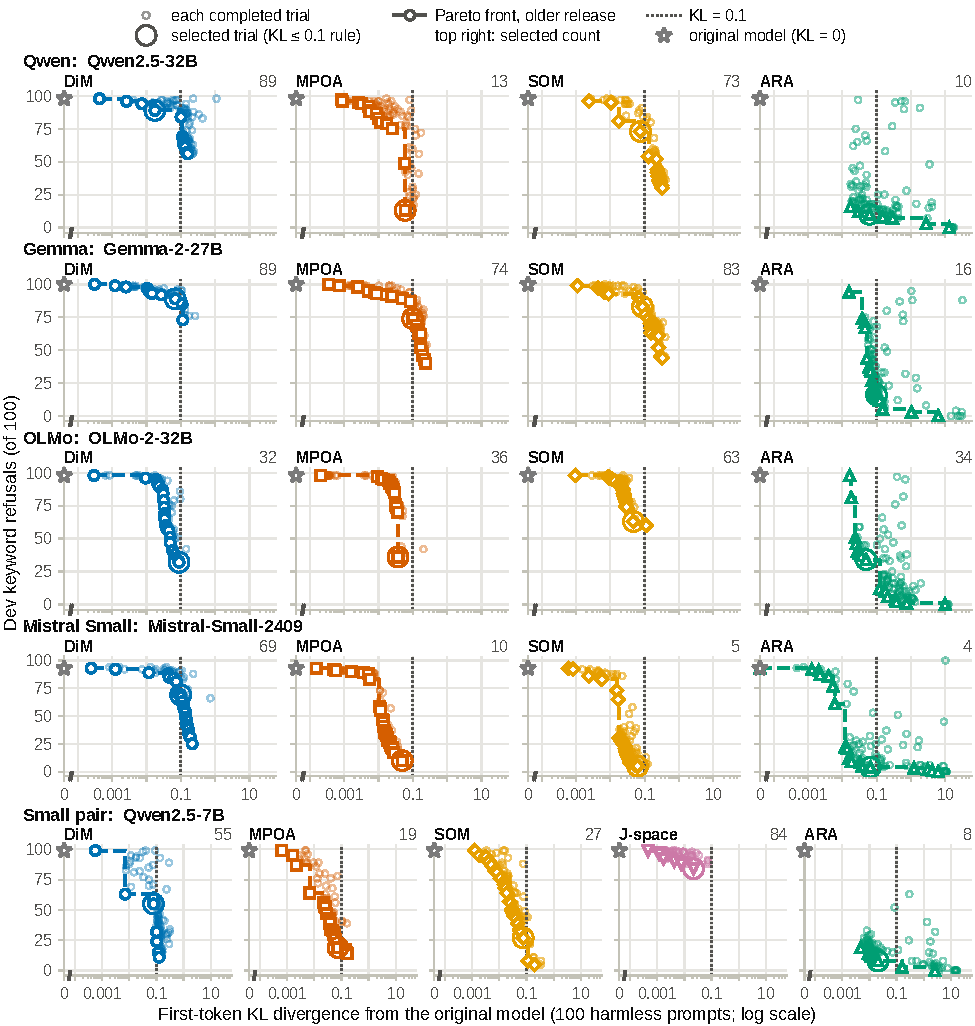
\includegraphics[width=\textwidth]{figures/figA1_trials_old_generation.pdf}
\caption{\textbf{All completed TPE trials of each optimisation run, older releases (dev set).} One panel per run (model $\times$ method, seed 1), laid out as in Figure~\ref{fig:pareto}; the older model of each pair heads its row. Each dot is one completed trial; the line is the run's Pareto front (dashed, hollow markers), the ring the trial chosen by the selection rule (fewest dev keyword refusals at KL $\le$ 0.1; count at the top right of the panel) and the grey star the original model (KL = 0). The x axis is logarithmic, with KL = 0 drawn at the left edge behind an axis break; the dotted line is the selection budget KL = 0.1. 2100 trials from 21 runs; the newer releases are in Figure~\ref{fig:trials-new}. Refusal counts are keyword matches on the 100 dev prompts that were also used for optimisation and selection, not held-out refusal rates.}
\label{fig:trials-old}
\end{figure*}
% caption: paper/figures/captions.md (figA1_trials_old_generation)

\begin{figure*}[tp]
\centering
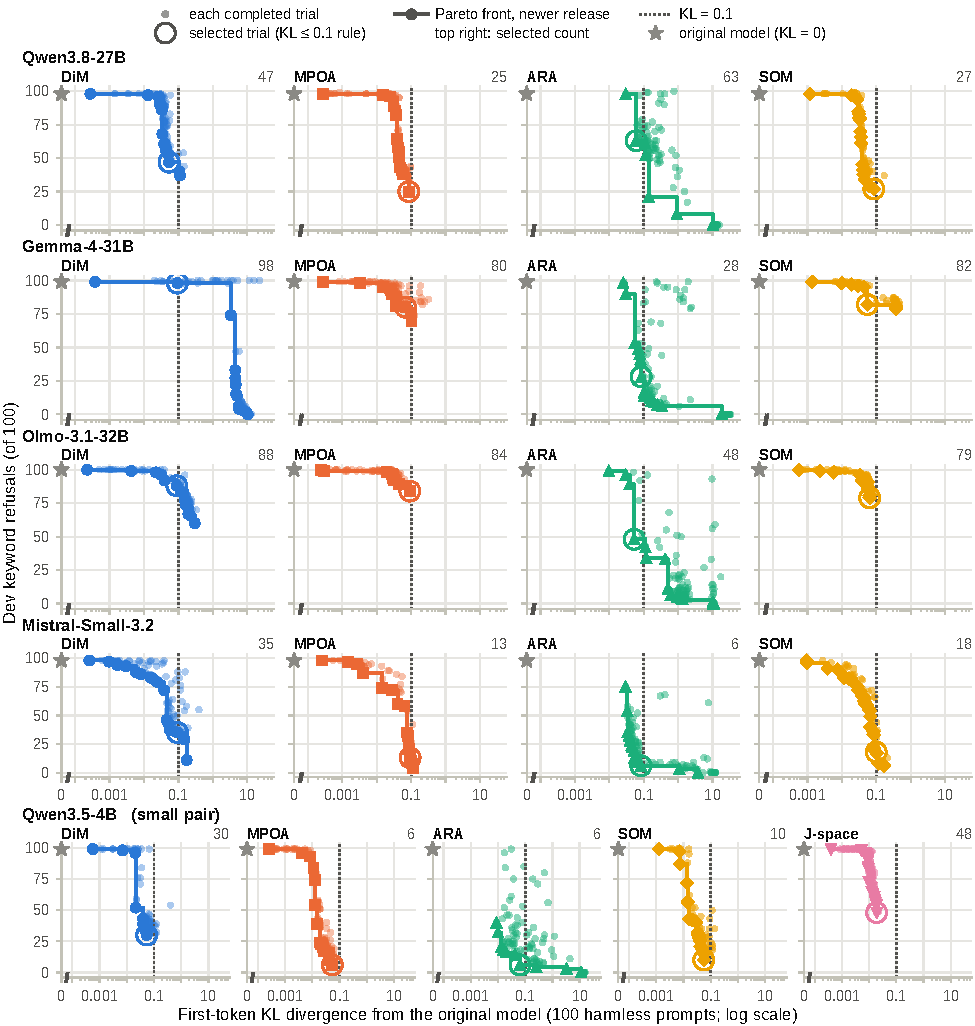
\includegraphics[width=\textwidth]{figures/figA2_trials_new_generation.pdf}
\caption{\textbf{All completed TPE trials of each optimisation run, newer releases (dev set).} One panel per run (model $\times$ method, seed 1), laid out as in Figure~\ref{fig:pareto}; the newer model of each pair heads its row. Each dot is one completed trial; the line is the run's Pareto front (solid, filled markers), the ring the trial chosen by the selection rule (fewest dev keyword refusals at KL $\le$ 0.1; count at the top right of the panel) and the grey star the original model (KL = 0). The x axis is logarithmic, with KL = 0 drawn at the left edge behind an axis break; the dotted line is the selection budget KL = 0.1. 2099 trials from 21 runs; the older releases are in Figure~\ref{fig:trials-old}. Refusal counts are keyword matches on the 100 dev prompts that were also used for optimisation and selection, not held-out refusal rates.}
\label{fig:trials-new}
\end{figure*}
% caption: paper/figures/captions.md (figA2_trials_new_generation)

\begin{figure*}[tp]
\centering
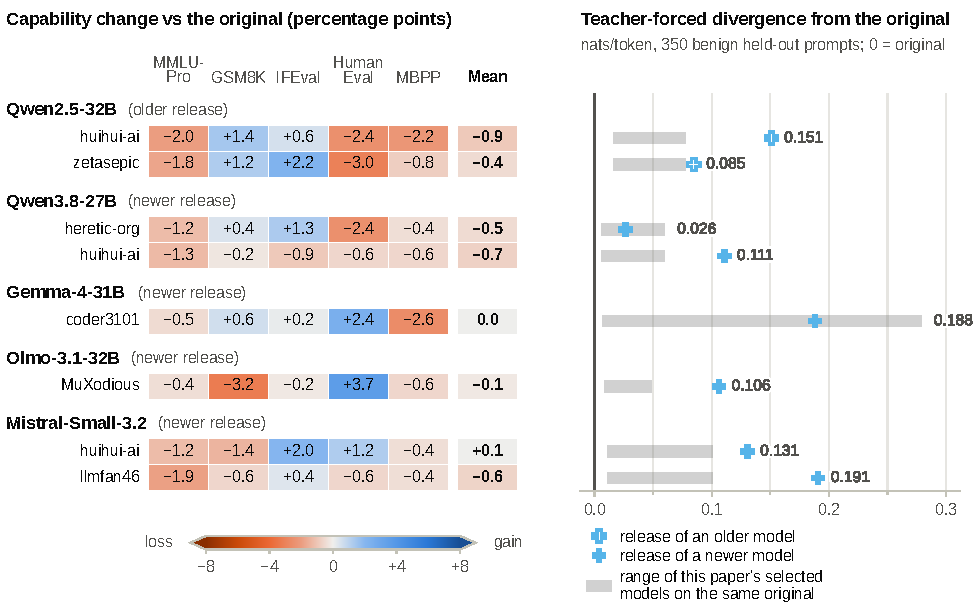
\includegraphics[width=\textwidth]{figures/figA3_community_releases.pdf}
\caption{\textbf{Public community releases: capability change and divergence from the original.} The 8 community releases evaluated alongside the selected models (2 of older, 6 of newer models; row label = Hugging Face uploader), grouped by the original they were derived from. Left: benchmark score minus that of the same original, in percentage points, with the diverging scale of Figure~\ref{fig:capability} (saturating at $\pm$8 pp; printed values exact); the last column is the unweighted mean of the five benchmarks. Right: teacher-forced divergence on the 350 benign held-out prompts, defined as in Figure~\ref{fig:divergence} (0 = the original); hollow markers are releases of the older, filled of the newer model of a pair. The grey bar spans the divergences of this paper's selected models on the same original (all conditions of Figure~\ref{fig:divergence}). 6 of 8 releases lie above that range; divergences range from 0.026 (heretic-org, Qwen3.8-27B) to 0.191 (llmfan46, Mistral-Small-3.2) nats per token, and mean capability changes from $-$0.9 to +0.1 pp. The releases were made by third parties with their own methods and selection; they were not selected with this paper's rule and are not part of the H1--H3 tests.}
\label{fig:community-releases}
\end{figure*}
% caption: paper/figures/captions.md (figA3_community_releases)

\begin{figure*}[tp]
\centering
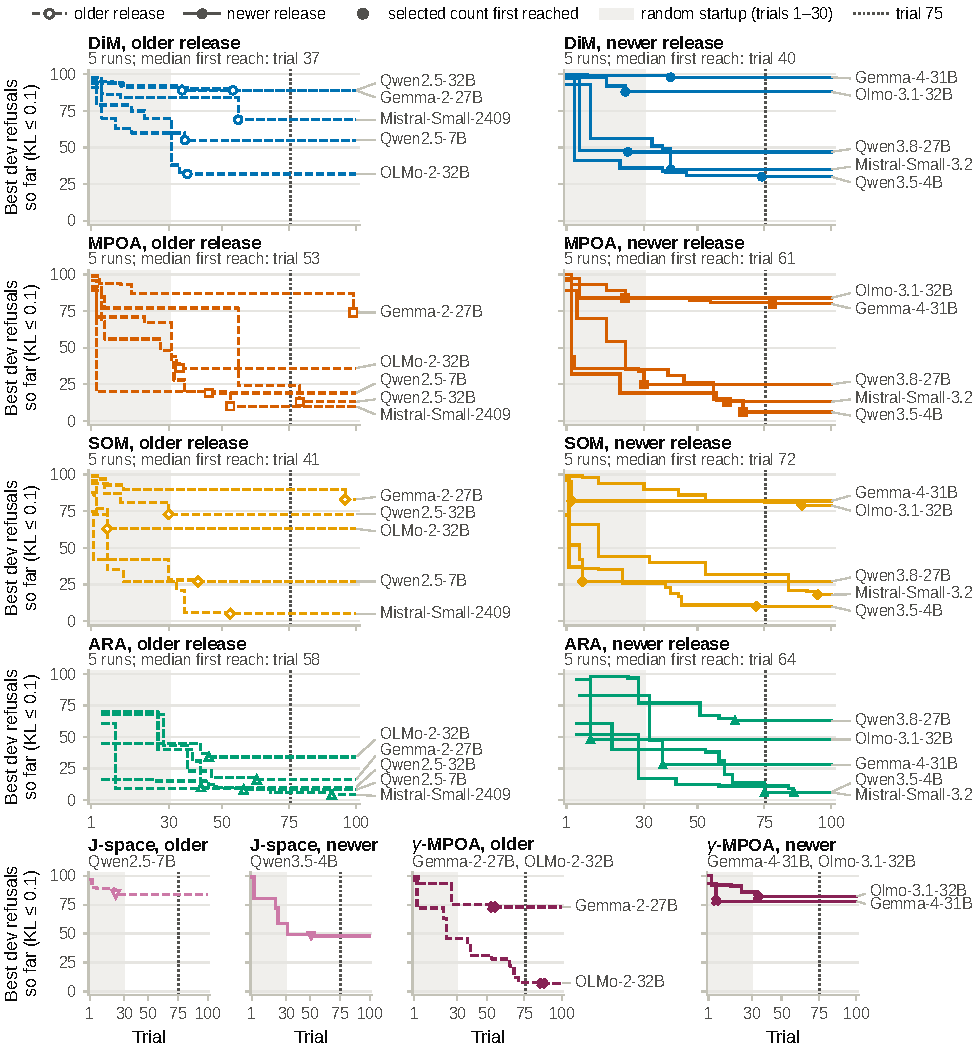
\includegraphics[width=\textwidth]{figures/figA4_search_convergence_runs.pdf}
\caption{\textbf{Search-budget convergence of every optimisation run (dev set).} One step curve per run (seed 1): after trial $t$, the fewest dev keyword refusals (of 100) among trials 1 to $t$ with first-token KL divergence $\le$ 0.1 from the original, i.e. the count the selection rule would have returned had the search stopped at trial $t$. Rows are methods and columns the older and newer release of each pair, so that a panel holds at most five runs, each named at its right end; bottom row: J-space (small pair only) and $\gamma$-MPOA (Gemma and OLMo pairs only). Dashed lines with hollow markers are older, solid lines with filled markers newer releases; the marker sits where the run first reached the count it finally selected. Curves start at the run's first trial within the KL budget (trials 5--10 for ARA, 1--2 otherwise). The grey band marks the 30 random startup trials of the TPE sampler, the dotted line trial 75. The medians, spreads and first-reach histogram of the core runs are in Figure~\ref{fig:search-convergence}. All counts are keyword matches on the 100 dev prompts that were also used for search and selection, not held-out refusal rates.}
\label{fig:search-runs}
\end{figure*}
% caption: paper/figures/captions.md (figA4_search_convergence_runs)

% Auto-generated by scripts/make_results_tables.py at 2026-11-06T06:33:50Z -- do not edit by hand.
\begin{table*}[t]
\centering\small
\caption{Keyword refusals on the development set (mlabonne/harmful\_behaviors, test split, first 100 prompts; count out of 100, Heretic keyword scorer) for the trial selected at each first-token KL budget $\tau$ (KL on mlabonne/harmless\_alpaca, test split, first 100 prompts). Selection rule: among completed trials with KL $\le\tau$, fewest refusals; ties broken by lower KL, then lower trial index. ``Original'' is the unmodified model as recorded by Heretic in the same runs. Main study; seed 1; 100 trials planned per run. $^\dagger$Run with fewer completed than planned trials (Qwen3.8-27B MPOA: 99 of 100). --: not yet available.}
\label{tab:dev-refusals-main}
\begin{tabular}{llrrrrrrrr}
\toprule
 & & \multicolumn{2}{c}{Qwen} & \multicolumn{2}{c}{Gemma} & \multicolumn{2}{c}{OLMo} & \multicolumn{2}{c}{Mistral Small} \\
\cmidrule(lr){3-4}\cmidrule(lr){5-6}\cmidrule(lr){7-8}\cmidrule(lr){9-10}
Method & $\tau$ & 2.5-32B & 3.8-27B & 2-27B & 4-31B & 2-32B & 3.1-32B & 2409 & 3.2-24B \\
\midrule
Original & & 98 & 98 & 100 & 99 & 98 & 100 & 93 & 98 \\
\midrule
DiM & 0.05 & 89 & 53 & 92 & 99 & 47 & 92 & 85 & 46 \\
 & 0.1 & 89 & 47 & 89 & 98 & 32 & 88 & 69 & 35 \\
 & 0.2 & 56 & 37 & 73 & 98 & 32 & 67 & 31 & 11 \\
\midrule
MPOA & 0.05 & 75 & 43$^\dagger$ & 89 & 81 & 36 & 89 & 10 & 60 \\
 & 0.1 & 13 & 25$^\dagger$ & 74 & 80 & 36 & 84 & 10 & 13 \\
 & 0.2 & 13 & 25$^\dagger$ & 46 & 70 & 36 & 84 & 10 & 4 \\
\midrule
ARA & 0.05 & 12 & 98 & 67 & 90 & 34 & 89 & 5 & 22 \\
 & 0.1 & 10 & 63 & 16 & 28 & 34 & 48 & 4 & 6 \\
 & 0.2 & 8 & 21 & 5 & 9 & 10 & 34 & 4 & 6 \\
\midrule
SOM & 0.05 & 81 & 34 & 93 & 95 & 63 & 92 & 8 & 60 \\
 & 0.1 & 73 & 27 & 83 & 82 & 63 & 79 & 5 & 18 \\
 & 0.2 & 54 & 27 & 63 & 82 & 60 & 79 & 5 & 6 \\
\bottomrule
\end{tabular}
\end{table*}
% src: paper/tables/t1_dev_refusals.csv (built from selection.json files; per-cell source_file column)
% src: runs/mc-h200-1/results/bench/mistral-small-2409__ara/selection.json, runs/mc-h200-1/results/bench/mistral-small-2409__dim/selection.json, runs/mc-h200-1/results/bench/mistral-small-2409__mpoa/selection.json, runs/mc-h200-1/results/bench/mistral-small-2409__som/selection.json, runs/mc-h200-1/results/bench/mistral-small-3.2__ara/selection.json, runs/mc-h200-1/results/bench/mistral-small-3.2__dim/selection.json, runs/mc-h200-1/results/bench/mistral-small-3.2__mpoa/selection.json, runs/mc-h200-1/results/bench/mistral-small-3.2__som/selection.json, runs/mc-h200-1/results/bench/olmo-2-32b__ara/selection.json, runs/mc-h200-1/results/bench/olmo-2-32b__dim/selection.json, runs/mc-h200-1/results/bench/olmo-2-32b__mpoa/selection.json, runs/mc-h200-1/results/bench/olmo-2-32b__som/selection.json, runs/mc-h200-1/results/bench/olmo-3.1-32b__ara/selection.json, runs/mc-h200-1/results/bench/olmo-3.1-32b__dim/selection.json, runs/mc-h200-1/results/bench/olmo-3.1-32b__mpoa/selection.json, runs/mc-h200-1/results/bench/olmo-3.1-32b__som/selection.json, runs/mc-rtx-1/results/bench/gemma-2-27b__ara/selection.json, runs/mc-rtx-1/results/bench/gemma-2-27b__dim/selection.json, runs/mc-rtx-1/results/bench/gemma-2-27b__mpoa/selection.json, runs/mc-rtx-1/results/bench/gemma-2-27b__som/selection.json, runs/mc-rtx-1/results/bench/gemma-4-31b__ara/selection.json, runs/mc-rtx-1/results/bench/gemma-4-31b__dim/selection.json, runs/mc-rtx-1/results/bench/gemma-4-31b__mpoa/selection.json, runs/mc-rtx-1/results/bench/gemma-4-31b__som/selection.json, runs/mc-rtx-1/results/bench/qwen2.5-32b__ara/selection.json, runs/mc-rtx-1/results/bench/qwen2.5-32b__dim/selection.json, runs/mc-rtx-1/results/bench/qwen2.5-32b__mpoa/selection.json, runs/mc-rtx-1/results/bench/qwen2.5-32b__som/selection.json, runs/mc-rtx-1/results/bench/qwen3.8-27b__ara/selection.json, runs/mc-rtx-1/results/bench/qwen3.8-27b__dim/selection.json, runs/mc-rtx-1/results/bench/qwen3.8-27b__mpoa/selection.json, runs/mc-rtx-1/results/bench/qwen3.8-27b__som/selection.json
% src: ../heretic/config.default.toml (KeywordRate: mlabonne/harmful_behaviors test[:100]; KLDivergence: mlabonne/harmless_alpaca test[:100]); scripts/select_trial.py (selection rule)
% src: seed, n_trials_planned, n_trials_complete: the selection.json files above (study settings stored in each Optuna journal); configs/core_{dim,mpoa,ara,som,jspace}.toml
% Missing cells rendered as '--' (status from the CSV):
%   none


% Auto-generated by scripts/make_results_tables.py at 2026-11-06T06:33:50Z -- do not edit by hand.
\begin{table}[t]
\centering\small
\caption{Keyword refusals on the development set (mlabonne/harmful\_behaviors, test split, first 100 prompts; count out of 100, Heretic keyword scorer) for the trial selected at each first-token KL budget $\tau$ (KL on mlabonne/harmless\_alpaca, test split, first 100 prompts). Selection rule: among completed trials with KL $\le\tau$, fewest refusals; ties broken by lower KL, then lower trial index. ``Original'' is the unmodified model as recorded by Heretic in the same runs. Small pair; seed 1; 100 trials planned per run. --: not yet available.}
\label{tab:dev-refusals-small}
\begin{tabular}{llrr}
\toprule
 & & \multicolumn{2}{c}{Qwen (small pair)} \\
\cmidrule(lr){3-4}
Method & $\tau$ & 2.5-7B & 3.5-4B \\
\midrule
Original & & 99 & 99 \\
\midrule
DiM & 0.05 & 63 & 34 \\
 & 0.1 & 55 & 30 \\
 & 0.2 & 11 & 30 \\
\midrule
MPOA & 0.05 & 33 & 10 \\
 & 0.1 & 19 & 6 \\
 & 0.2 & 14 & 6 \\
\midrule
ARA & 0.05 & 8 & 14 \\
 & 0.1 & 8 & 6 \\
 & 0.2 & 3 & 6 \\
\midrule
SOM & 0.05 & 39 & 19 \\
 & 0.1 & 27 & 10 \\
 & 0.2 & 5 & 10 \\
\midrule
J-space & 0.05 & 84 & 48 \\
 & 0.1 & 84 & 48 \\
 & 0.2 & 84 & 48 \\
\bottomrule
\end{tabular}
\end{table}
% src: paper/tables/t1_dev_refusals.csv (built from selection.json files; per-cell source_file column)
% src: results/bench-4090/qwen2.5-7b__ara/selection.json, results/bench-4090/qwen2.5-7b__dim/selection.json, results/bench-4090/qwen2.5-7b__jspace/selection.json, results/bench-4090/qwen2.5-7b__mpoa/selection.json, results/bench-4090/qwen2.5-7b__som/selection.json, results/bench-4090/qwen3.5-4b__ara/selection.json, results/bench-4090/qwen3.5-4b__dim/selection.json, results/bench-4090/qwen3.5-4b__jspace/selection.json, results/bench-4090/qwen3.5-4b__mpoa/selection.json, results/bench-4090/qwen3.5-4b__som/selection.json
% src: ../heretic/config.default.toml (KeywordRate: mlabonne/harmful_behaviors test[:100]; KLDivergence: mlabonne/harmless_alpaca test[:100]); scripts/select_trial.py (selection rule)
% src: seed, n_trials_planned, n_trials_complete: the selection.json files above (study settings stored in each Optuna journal); configs/core_{dim,mpoa,ara,som,jspace}.toml
% Missing cells rendered as '--' (status from the CSV):
%   none


% t2_capability_main.tex is 60pt wider than the text at \footnotesize; it is auto-generated (do not edit), so it
% is set here with narrower column gaps and a 7.5pt font, local to this group.
{\setlength{\tabcolsep}{3pt}\renewcommand{\footnotesize}{\fontsize{7.5}{9}\selectfont}%
% Auto-generated by scripts/make_results_tables.py at 2026-11-06T06:33:50Z -- do not edit by hand.
\begin{table*}[t]
\centering\footnotesize
\caption{Capability of the original and the selected modified models (KL $\le 0.1$ trial), in \%. Modified models: score with the difference to the same family's original model in percentage points in parentheses (computed from unrounded scores). Number of items in the column header. Metrics: MMLU-Pro exact match (custom extract, 5-shot CoT); GSM8K exact match (flexible extract, 5-shot); IFEval prompt-level strict accuracy (0-shot); HumanEval pass@1 (0-shot); MBPP pass@1 (3-shot). Greedy decoding, chat template on, thinking disabled. Main study. $^\ddagger$Rescored from the logged samples with the patched MBPP answer extractor (run predates the lm-eval patch; scripts/bench/LM\_EVAL\_PATCHES.md): Qwen2.5-32B-Instruct Original MBPP. $^\S$Original model's capability run used evaluation-harness settings that differ from its modified models' runs (original vs.\ modified models; per-cell settings in paper/tables/coverage.md, evaluation protocol table): Qwen2.5-32B-Instruct: bench.py revision (sha256 prefix) 0ac2aca202 vs.\ b6a926cf73, f220db7bb9; output post-processing none vs.\ U+2581$\rightarrow$space; BENCH\_VLLM\_EXTRA unset vs.\ \{\}. gemma-2-27b-it: bench.py revision (sha256 prefix) b6a926cf73 vs.\ f220db7bb9. --: not yet available.}
\label{tab:capability-main}
\begin{tabular}{llrrrrr}
\toprule
Model & Method & MMLU-Pro (1000) & GSM8K (500) & IFEval (541) & HumanEval (164) & MBPP (500) \\
\midrule
Qwen2.5-32B-Instruct & Original$^\S$ & 71.1 & 85.4 & 78.9 & 89.6 & 77.6$^\ddagger$ \\
 & DiM & 69.9\,($-$1.2) & 85.6\,(+0.2) & 79.7\,(+0.7) & 90.2\,(+0.6) & 77.0\,($-$0.6) \\
 & MPOA & 70.5\,($-$0.6) & 85.0\,($-$0.4) & 80.8\,(+1.8) & 89.6\,(0.0) & 76.6\,($-$1.0) \\
 & ARA & 70.3\,($-$0.8) & 86.6\,(+1.2) & 79.9\,(+0.9) & 84.8\,($-$4.9) & 77.0\,($-$0.6) \\
 & SOM & 71.1\,(0.0) & 85.6\,(+0.2) & 79.5\,(+0.6) & 89.6\,(0.0) & 78.4\,(+0.8) \\
\midrule
Qwen3.8-27B & Original & 79.6 & 96.2 & 80.6 & 97.6 & 80.8 \\
 & DiM & 79.5\,($-$0.1) & 96.6\,(+0.4) & 80.6\,(0.0) & 96.3\,($-$1.2) & 80.6\,($-$0.2) \\
 & MPOA & 79.6\,(0.0) & 97.0\,(+0.8) & 82.4\,(+1.8) & 97.0\,($-$0.6) & 80.4\,($-$0.4) \\
 & ARA & 78.5\,($-$1.1) & 95.8\,($-$0.4) & 81.0\,(+0.4) & 93.9\,($-$3.7) & 79.2\,($-$1.6) \\
 & SOM & 79.4\,($-$0.2) & 97.0\,(+0.8) & 79.5\,($-$1.1) & 95.1\,($-$2.4) & 80.6\,($-$0.2) \\
\midrule
gemma-2-27b-it & Original$^\S$ & 42.8 & 86.4 & 60.6 & 76.2 & 69.6 \\
 & DiM & 42.3\,($-$0.5) & 86.0\,($-$0.4) & 60.6\,(0.0) & 75.0\,($-$1.2) & 69.2\,($-$0.4) \\
 & MPOA & 43.1\,(+0.3) & 84.4\,($-$2.0) & 60.8\,(+0.2) & 76.8\,(+0.6) & 68.6\,($-$1.0) \\
 & ARA & 44.3\,(+1.5) & 84.2\,($-$2.2) & 61.4\,(+0.7) & 76.8\,(+0.6) & 70.0\,(+0.4) \\
 & SOM & 45.3\,(+2.5) & 86.2\,($-$0.2) & 60.8\,(+0.2) & 75.6\,($-$0.6) & 68.6\,($-$1.0) \\
\midrule
gemma-4-31B-it & Original & 85.6 & 96.6 & 91.5 & 92.7 & 71.4 \\
 & DiM & 85.2\,($-$0.4) & 97.0\,(+0.4) & 90.0\,($-$1.5) & 90.2\,($-$2.4) & 69.2\,($-$2.2) \\
 & MPOA & 86.1\,(+0.5) & 96.4\,($-$0.2) & 91.7\,(+0.2) & 90.9\,($-$1.8) & 70.0\,($-$1.4) \\
 & ARA & 85.2\,($-$0.4) & 97.0\,(+0.4) & 91.5\,(0.0) & 86.0\,($-$6.7) & 67.2\,($-$4.2) \\
 & SOM & 85.4\,($-$0.2) & 96.8\,(+0.2) & 89.6\,($-$1.8) & 89.0\,($-$3.7) & 63.0\,($-$8.4) \\
\midrule
OLMo-2-0325-32B-Instruct & Original & 52.6 & 88.8 & 84.3 & 61.0 & 44.0 \\
 & DiM & 52.2\,($-$0.4) & 88.6\,($-$0.2) & 80.8\,($-$3.5) & 59.8\,($-$1.2) & 38.4\,($-$5.6) \\
 & MPOA & 52.3\,($-$0.3) & 88.0\,($-$0.8) & 83.0\,($-$1.3) & 57.9\,($-$3.0) & 42.2\,($-$1.8) \\
 & ARA & 52.3\,($-$0.3) & 88.6\,($-$0.2) & 80.6\,($-$3.7) & 57.3\,($-$3.7) & 30.8\,($-$13.2) \\
 & SOM & 51.9\,($-$0.7) & 88.2\,($-$0.6) & 83.2\,($-$1.1) & 57.9\,($-$3.0) & 44.0\,(0.0) \\
\midrule
Olmo-3.1-32B-Instruct & Original & 64.7 & 89.2 & 86.9 & 87.2 & 71.4 \\
 & DiM & 64.6\,($-$0.1) & 90.4\,(+1.2) & 87.2\,(+0.4) & 88.4\,(+1.2) & 70.2\,($-$1.2) \\
 & MPOA & 63.5\,($-$1.2) & 89.8\,(+0.6) & 86.7\,($-$0.2) & 90.2\,(+3.0) & 71.4\,(0.0) \\
 & ARA & 63.5\,($-$1.2) & 88.6\,($-$0.6) & 87.2\,(+0.4) & 92.1\,(+4.9) & 70.0\,($-$1.4) \\
 & SOM & 64.1\,($-$0.6) & 89.2\,(0.0) & 86.7\,($-$0.2) & 91.5\,(+4.3) & 70.8\,($-$0.6) \\
\midrule
Mistral-Small-Instruct-2409 & Original & 56.2 & 88.2 & 61.4 & 76.2 & 62.6 \\
 & DiM & 56.6\,(+0.4) & 87.4\,($-$0.8) & 62.3\,(+0.9) & 75.6\,($-$0.6) & 61.6\,($-$1.0) \\
 & MPOA & 53.9\,($-$2.3) & 88.0\,($-$0.2) & 61.0\,($-$0.4) & 75.0\,($-$1.2) & 62.2\,($-$0.4) \\
 & ARA & 51.5\,($-$4.7) & 84.2\,($-$4.0) & 63.6\,(+2.2) & 74.4\,($-$1.8) & 58.0\,($-$4.6) \\
 & SOM & 55.6\,($-$0.6) & 88.0\,($-$0.2) & 63.2\,(+1.8) & 76.8\,(+0.6) & 62.4\,($-$0.2) \\
\midrule
Mistral-Small-3.2-24B-Instruct-2506 & Original & 64.8 & 93.6 & 77.1 & 87.2 & 70.6 \\
 & DiM & 64.8\,(0.0) & 93.8\,(+0.2) & 76.9\,($-$0.2) & 87.8\,(+0.6) & 71.2\,(+0.6) \\
 & MPOA & 64.9\,(+0.1) & 94.0\,(+0.4) & 76.0\,($-$1.1) & 89.6\,(+2.4) & 69.6\,($-$1.0) \\
 & ARA & 63.4\,($-$1.4) & 92.6\,($-$1.0) & 77.4\,(+0.4) & 88.4\,(+1.2) & 70.2\,($-$0.4) \\
 & SOM & 63.7\,($-$1.1) & 93.6\,(0.0) & 76.0\,($-$1.1) & 88.4\,(+1.2) & 69.6\,($-$1.0) \\
\bottomrule
\end{tabular}
\end{table*}
% src: paper/tables/t2_capability.csv (built from summary.json 'benchmarks'; per-cell source_file column)
% src: runs/mc-h200-1/results/bench/mistral-small-2409__ara/summary.json, runs/mc-h200-1/results/bench/mistral-small-2409__base/summary.json, runs/mc-h200-1/results/bench/mistral-small-2409__dim/summary.json, runs/mc-h200-1/results/bench/mistral-small-2409__mpoa/summary.json, runs/mc-h200-1/results/bench/mistral-small-2409__som/summary.json, runs/mc-h200-1/results/bench/mistral-small-3.2__ara/summary.json, runs/mc-h200-1/results/bench/mistral-small-3.2__base/summary.json, runs/mc-h200-1/results/bench/mistral-small-3.2__dim/summary.json, runs/mc-h200-1/results/bench/mistral-small-3.2__mpoa/summary.json, runs/mc-h200-1/results/bench/mistral-small-3.2__som/summary.json, runs/mc-h200-1/results/bench/olmo-2-32b__ara/summary.json, runs/mc-h200-1/results/bench/olmo-2-32b__base/summary.json, runs/mc-h200-1/results/bench/olmo-2-32b__dim/summary.json, runs/mc-h200-1/results/bench/olmo-2-32b__mpoa/summary.json, runs/mc-h200-1/results/bench/olmo-2-32b__som/summary.json, runs/mc-h200-1/results/bench/olmo-3.1-32b__ara/summary.json, runs/mc-h200-1/results/bench/olmo-3.1-32b__base/summary.json, runs/mc-h200-1/results/bench/olmo-3.1-32b__dim/summary.json, runs/mc-h200-1/results/bench/olmo-3.1-32b__mpoa/summary.json, runs/mc-h200-1/results/bench/olmo-3.1-32b__som/summary.json, runs/mc-rtx-1/results/bench/gemma-2-27b__ara/summary.json, runs/mc-rtx-1/results/bench/gemma-2-27b__base/summary.json, runs/mc-rtx-1/results/bench/gemma-2-27b__dim/summary.json, runs/mc-rtx-1/results/bench/gemma-2-27b__mpoa/summary.json, runs/mc-rtx-1/results/bench/gemma-2-27b__som/summary.json, runs/mc-rtx-1/results/bench/gemma-4-31b__ara/summary.json, runs/mc-rtx-1/results/bench/gemma-4-31b__base/summary.json, runs/mc-rtx-1/results/bench/gemma-4-31b__dim/summary.json, runs/mc-rtx-1/results/bench/gemma-4-31b__mpoa/summary.json, runs/mc-rtx-1/results/bench/gemma-4-31b__som/summary.json, runs/mc-rtx-1/results/bench/qwen2.5-32b__ara/summary.json, runs/mc-rtx-1/results/bench/qwen2.5-32b__base/summary.json, runs/mc-rtx-1/results/bench/qwen2.5-32b__dim/summary.json, runs/mc-rtx-1/results/bench/qwen2.5-32b__mpoa/summary.json, runs/mc-rtx-1/results/bench/qwen2.5-32b__som/summary.json, runs/mc-rtx-1/results/bench/qwen3.8-27b__ara/summary.json, runs/mc-rtx-1/results/bench/qwen3.8-27b__base/summary.json, runs/mc-rtx-1/results/bench/qwen3.8-27b__dim/summary.json, runs/mc-rtx-1/results/bench/qwen3.8-27b__mpoa/summary.json, runs/mc-rtx-1/results/bench/qwen3.8-27b__som/summary.json
% src: scripts/bench/README.md (protocol: metrics, shots, decoding, chat template, thinking off); metric names and n: summary.json 'benchmarks' (metric, n)
% src (section-sign footnote): summary.json versions['sha256:bench.py'], postprocess, versions.env, backend, lm_kwargs, versions of runs/mc-rtx-1/results/bench/qwen2.5-32b__base/summary.json, runs/mc-rtx-1/results/bench/gemma-2-27b__base/summary.json vs. the modified models' summary.json; paper/tables/coverage.md (evaluation protocol table)
% Missing cells rendered as '--' (status from the CSV):
%   none

}

% Auto-generated by scripts/make_results_tables.py at 2026-11-06T06:33:50Z -- do not edit by hand.
\begin{table*}[t]
\centering\small
\caption{Capability of the original and the selected modified models (KL $\le 0.1$ trial), in \%. Modified models: score with the difference to the same family's original model in percentage points in parentheses (computed from unrounded scores). Number of items in the column header. Metrics: MMLU-Pro exact match (custom extract, 5-shot CoT); GSM8K exact match (flexible extract, 5-shot); IFEval prompt-level strict accuracy (0-shot); HumanEval pass@1 (0-shot); MBPP pass@1 (3-shot). Greedy decoding, chat template on, thinking disabled. Small pair. --: not yet available.}
\label{tab:capability-small}
\setlength{\tabcolsep}{4pt}
\begin{tabular}{llrrrrr}
\toprule
Model & Method & MMLU-Pro (1000) & GSM8K (500) & IFEval (541) & HumanEval (164) & MBPP (500) \\
\midrule
Qwen2.5-7B-Instruct & Original & 59.5 & 85.8 & 71.2 & 84.8 & 63.2 \\
 & DiM & 58.1\,($-$1.4) & 86.0\,(+0.2) & 71.7\,(+0.6) & 86.0\,(+1.2) & 63.8\,(+0.6) \\
 & MPOA & 57.9\,($-$1.6) & 85.0\,($-$0.8) & 70.6\,($-$0.6) & 86.6\,(+1.8) & 63.2\,(0.0) \\
 & ARA & 57.8\,($-$1.7) & 86.8\,(+1.0) & 70.2\,($-$0.9) & 87.2\,(+2.4) & 64.8\,(+1.6) \\
 & SOM & 59.8\,(+0.3) & 84.0\,($-$1.8) & 70.6\,($-$0.6) & 83.5\,($-$1.2) & 64.8\,(+1.6) \\
 & J-space & 60.5\,(+1.0) & 86.4\,(+0.6) & 72.6\,(+1.5) & 84.8\,(0.0) & 64.4\,(+1.2) \\
\midrule
Qwen3.5-4B & Original & 70.6 & 91.8 & 82.3 & 79.9 & 62.6 \\
 & DiM & 70.1\,($-$0.5) & 91.2\,($-$0.6) & 82.4\,(+0.2) & 81.7\,(+1.8) & 61.8\,($-$0.8) \\
 & MPOA & 69.2\,($-$1.4) & 91.6\,($-$0.2) & 82.3\,(0.0) & 79.9\,(0.0) & 61.6\,($-$1.0) \\
 & ARA & 69.4\,($-$1.2) & 90.2\,($-$1.6) & 79.3\,($-$3.0) & 79.3\,($-$0.6) & 61.2\,($-$1.4) \\
 & SOM & 68.7\,($-$1.9) & 92.6\,(+0.8) & 81.7\,($-$0.6) & 79.9\,(0.0) & 61.2\,($-$1.4) \\
 & J-space & 70.4\,($-$0.2) & 91.6\,($-$0.2) & 81.3\,($-$0.9) & 82.9\,(+3.0) & 61.2\,($-$1.4) \\
\bottomrule
\end{tabular}
\end{table*}
% src: paper/tables/t2_capability.csv (built from summary.json 'benchmarks'; per-cell source_file column)
% src: results/bench-4090/qwen2.5-7b__ara/summary.json, results/bench-4090/qwen2.5-7b__base/summary.json, results/bench-4090/qwen2.5-7b__dim/summary.json, results/bench-4090/qwen2.5-7b__jspace/summary.json, results/bench-4090/qwen2.5-7b__mpoa/summary.json, results/bench-4090/qwen2.5-7b__som/summary.json, results/bench-4090/qwen3.5-4b__ara/summary.json, results/bench-4090/qwen3.5-4b__base/summary.json, results/bench-4090/qwen3.5-4b__dim/summary.json, results/bench-4090/qwen3.5-4b__jspace/summary.json, results/bench-4090/qwen3.5-4b__mpoa/summary.json, results/bench-4090/qwen3.5-4b__som/summary.json
% src: scripts/bench/README.md (protocol: metrics, shots, decoding, chat template, thinking off); metric names and n: summary.json 'benchmarks' (metric, n)
% Missing cells rendered as '--' (status from the CSV):
%   none


% Auto-generated by scripts/make_results_tables.py at 2026-11-06T06:33:50Z -- do not edit by hand.
\begin{table*}[t]
\centering\small
\caption{Teacher-forced log-likelihood of the original model's greedy answers to the 350 benign held-out prompts (jbb\_benign 100, xstest\_safe 250). ``Original'': mean log-probability per answer token under the original model (token-weighted over all items); method columns: the same quantity under the selected modified model (KL $\le 0.1$ trial) minus the original's value (negative = the original answers became less likely). Tokens: number of scored answer tokens. Main study. $^\S$Original model's held-out generation and teacher forcing come from a run whose evaluation-harness settings differ from its modified models' runs (original vs.\ modified models; per-cell settings in paper/tables/coverage.md, evaluation protocol table): Qwen2.5-32B-Instruct: separate bench.py run (refusal\_run/summary.json in its evaluation directory); bench.py revision (sha256 prefix) f7731f7d3f vs.\ b6a926cf73, f220db7bb9; output post-processing none vs.\ U+2581$\rightarrow$space. gemma-2-27b-it: bench.py revision (sha256 prefix) b6a926cf73 vs.\ f220db7bb9. --: not yet available.}
\label{tab:teacher-forced-main}
\begin{tabular}{lrrrrrr}
\toprule
 & & & \multicolumn{4}{c}{Shift vs.\ original} \\
\cmidrule(lr){4-7}
Model & Tokens & Original & DiM & MPOA & ARA & SOM \\
\midrule
Qwen2.5-32B-Instruct & 112398 & $-$0.272$^\S$ & $-$0.017 & $-$0.042 & $-$0.077 & $-$0.020 \\
Qwen3.8-27B & 138016 & $-$0.275 & $-$0.006 & $-$0.060 & $-$0.042 & $-$0.021 \\
gemma-2-27b-it & 97666 & $-$0.227$^\S$ & $-$0.068 & $-$0.063 & $-$0.161 & $-$0.031 \\
gemma-4-31B-it & 142322 & $-$0.110 & $-$0.042 & $-$0.007 & $-$0.279 & $-$0.026 \\
OLMo-2-0325-32B-Instruct & 110792 & $-$0.520 & $-$0.051 & $-$0.088 & $-$0.055 & $-$0.030 \\
Olmo-3.1-32B-Instruct & 136772 & $-$0.288 & $-$0.008 & $-$0.008 & $-$0.049 & $-$0.016 \\
Mistral-Small-Instruct-2409 & 129960 & $-$0.209 & $-$0.004 & $-$0.018 & $-$0.080 & $-$0.023 \\
Mistral-Small-3.2-24B-Instruct-2506 & 131780 & $-$0.171 & $-$0.011 & $-$0.066 & $-$0.101 & $-$0.037 \\
\bottomrule
\end{tabular}
\end{table*}
% src: paper/tables/t3_teacher_forced.csv (summary.json 'teacher_forced'; per-cell source_file column)
% src: runs/mc-h200-1/results/bench/mistral-small-2409__ara/summary.json, runs/mc-h200-1/results/bench/mistral-small-2409__base/summary.json, runs/mc-h200-1/results/bench/mistral-small-2409__dim/summary.json, runs/mc-h200-1/results/bench/mistral-small-2409__mpoa/summary.json, runs/mc-h200-1/results/bench/mistral-small-2409__som/summary.json, runs/mc-h200-1/results/bench/mistral-small-3.2__ara/summary.json, runs/mc-h200-1/results/bench/mistral-small-3.2__base/summary.json, runs/mc-h200-1/results/bench/mistral-small-3.2__dim/summary.json, runs/mc-h200-1/results/bench/mistral-small-3.2__mpoa/summary.json, runs/mc-h200-1/results/bench/mistral-small-3.2__som/summary.json, runs/mc-h200-1/results/bench/olmo-2-32b__ara/summary.json, runs/mc-h200-1/results/bench/olmo-2-32b__base/summary.json, runs/mc-h200-1/results/bench/olmo-2-32b__dim/summary.json, runs/mc-h200-1/results/bench/olmo-2-32b__mpoa/summary.json, runs/mc-h200-1/results/bench/olmo-2-32b__som/summary.json, runs/mc-h200-1/results/bench/olmo-3.1-32b__ara/summary.json, runs/mc-h200-1/results/bench/olmo-3.1-32b__base/summary.json, runs/mc-h200-1/results/bench/olmo-3.1-32b__dim/summary.json, runs/mc-h200-1/results/bench/olmo-3.1-32b__mpoa/summary.json, runs/mc-h200-1/results/bench/olmo-3.1-32b__som/summary.json, runs/mc-rtx-1/results/bench/gemma-2-27b__ara/summary.json, runs/mc-rtx-1/results/bench/gemma-2-27b__base/summary.json, runs/mc-rtx-1/results/bench/gemma-2-27b__dim/summary.json, runs/mc-rtx-1/results/bench/gemma-2-27b__mpoa/summary.json, runs/mc-rtx-1/results/bench/gemma-2-27b__som/summary.json, runs/mc-rtx-1/results/bench/gemma-4-31b__ara/summary.json, runs/mc-rtx-1/results/bench/gemma-4-31b__base/summary.json, runs/mc-rtx-1/results/bench/gemma-4-31b__dim/summary.json, runs/mc-rtx-1/results/bench/gemma-4-31b__mpoa/summary.json, runs/mc-rtx-1/results/bench/gemma-4-31b__som/summary.json, runs/mc-rtx-1/results/bench/qwen2.5-32b__ara/summary.json, runs/mc-rtx-1/results/bench/qwen2.5-32b__base/refusal_run/summary.json, runs/mc-rtx-1/results/bench/qwen2.5-32b__dim/summary.json, runs/mc-rtx-1/results/bench/qwen2.5-32b__mpoa/summary.json, runs/mc-rtx-1/results/bench/qwen2.5-32b__som/summary.json, runs/mc-rtx-1/results/bench/qwen3.8-27b__ara/summary.json, runs/mc-rtx-1/results/bench/qwen3.8-27b__base/summary.json, runs/mc-rtx-1/results/bench/qwen3.8-27b__dim/summary.json, runs/mc-rtx-1/results/bench/qwen3.8-27b__mpoa/summary.json, runs/mc-rtx-1/results/bench/qwen3.8-27b__som/summary.json
% src: scripts/bench/bench.py (teacher_forced_logprobs: token-weighted mean over benign items); scripts/bench/refusal_sets.json (benign item counts)
% src (section-sign footnote): settings recorded in runs/mc-rtx-1/results/bench/qwen2.5-32b__base/refusal_run/summary.json, runs/mc-rtx-1/results/bench/gemma-2-27b__base/summary.json vs. the modified models' summary.json; paper/tables/coverage.md (evaluation protocol table)
% Missing cells rendered as '--' (status from the CSV):
%   none


% Auto-generated by scripts/make_results_tables.py at 2026-11-06T06:33:50Z -- do not edit by hand.
\begin{table*}[t]
\centering\small
\caption{Teacher-forced log-likelihood of the original model's greedy answers to the 350 benign held-out prompts (jbb\_benign 100, xstest\_safe 250). ``Original'': mean log-probability per answer token under the original model (token-weighted over all items); method columns: the same quantity under the selected modified model (KL $\le 0.1$ trial) minus the original's value (negative = the original answers became less likely). Tokens: number of scored answer tokens. Small pair. --: not yet available.}
\label{tab:teacher-forced-small}
\begin{tabular}{lrrrrrrr}
\toprule
 & & & \multicolumn{5}{c}{Shift vs.\ original} \\
\cmidrule(lr){4-8}
Model & Tokens & Original & DiM & MPOA & ARA & SOM & J-space \\
\midrule
Qwen2.5-7B-Instruct & 119254 & $-$0.321 & $-$0.019 & $-$0.018 & $-$0.048 & $-$0.026 & $-$0.009 \\
Qwen3.5-4B & 139372 & $-$0.412 & $-$0.010 & $-$0.031 & $-$0.093 & $-$0.035 & $-$0.045 \\
\bottomrule
\end{tabular}
\end{table*}
% src: paper/tables/t3_teacher_forced.csv (summary.json 'teacher_forced'; per-cell source_file column)
% src: results/bench-4090/qwen2.5-7b__ara/summary.json, results/bench-4090/qwen2.5-7b__base/summary.json, results/bench-4090/qwen2.5-7b__dim/summary.json, results/bench-4090/qwen2.5-7b__jspace/summary.json, results/bench-4090/qwen2.5-7b__mpoa/summary.json, results/bench-4090/qwen2.5-7b__som/summary.json, results/bench-4090/qwen3.5-4b__ara/summary.json, results/bench-4090/qwen3.5-4b__base/summary.json, results/bench-4090/qwen3.5-4b__dim/summary.json, results/bench-4090/qwen3.5-4b__jspace/summary.json, results/bench-4090/qwen3.5-4b__mpoa/summary.json, results/bench-4090/qwen3.5-4b__som/summary.json
% src: scripts/bench/bench.py (teacher_forced_logprobs: token-weighted mean over benign items); scripts/bench/refusal_sets.json (benign item counts)
% Missing cells rendered as '--' (status from the CSV):
%   none


% ---------------------------------------------------------------------
% 2026-11-10 ARS re-review revision (NEW-6): diagnosis of the failed Gemma-4-31B DiM edit, replacing the unsupported
% "plausibly for architectural reasons".
% src: scripts/analysis/postnorm_gain_scan.py -> results/analysis/gemma4_dim_kl_bands.csv (from the Optuna journal
% src: runs/mc-h200-1/runs/gemma-4-31b__dim__core-s1/checkpoints/google--gemma-4-31B-it.jsonl) and
% src: results/analysis/postnorm_gain_scan.csv (post-norm weights read from the base-model safetensors on Hugging Face);
% src: results/analysis/review_sel_kl_runs.csv (kl_of_best_above_cap: every other direction-based primary run <= 0.371).
\subsection{The Failed Gemma-4-31B DiM Edit}
\label{app:gemma4-dim}
In the Gemma-4-31B DiM study, 10 of the 100 trials met the KL cap and 90
exceeded it. Every trial with a first-token KL below 3 (28 trials) refused 98
to 100 of the 100 dev prompts; lower refusal appeared only above a KL of 3
(minimum 3 of 100 between 3 and 8, and 0 above 8), where the edited model is
far from the original. In every other direction-based primary study, the
lowest-refusal trial above the cap had a KL of at most 0.37. The edit therefore
did not trade refusal against divergence gradually: within any usable budget it
had no effect. Two mechanisms proposed for similar failures on Gemma-3 are a
residual-stream coordinate of very large magnitude that dominates the
difference-in-means estimate \cite{mishra2026onecoordinate,lai2025mpoa} and
learned normalisation gains that amplify it \cite{mishra2026onecoordinate}. The
post-sublayer RMSNorm gains of the four post-norm models were therefore read
from the released weights. Gemma-2-27B and Gemma-4-31B both had recurring
outlier channels (a gain over 20 times the layer's median in 39 of 92 and 27 of
120 post-norm vectors, mostly one channel in Gemma-2-27B and two in
Gemma-4-31B), whereas OLMo-2-32B and Olmo-3.1-32B had 3 of 128 and 1 of 128.
The median coefficient of variation of the gains was 0.65 and 0.68 for the
attention outputs and 0.38 and 0.62 for the feed-forward outputs of the two
Gemma models, and 0.09 to 0.34 in the OLMo models; outlier channels were more
frequent in Gemma-2-27B than in Gemma-4-31B (42\% and 23\% of vectors). The gains thus separate the Gemma family from
OLMo, consistent with the larger effect of the $\gamma$ correction on the Gemma
models (\S\ref{sec:res-secondary}), but they do not separate Gemma-4-31B from
Gemma-2-27B, on which DiM lowered refusal. The activation outlier was not
measured, and the cause of the failure remains untested.

% \clearpage (integration, 2026-11-06): flushes the figures and tables of 08d before D.1, so that Tables
% tab:trunc256, tab:dev-rescore and tab:dev-rescore-gemma2 appear next to their text instead of after all of 08d's floats.
\clearpage
% ============================================================
% APPENDIX -- JUDGING THE FIRST 256 TOKENS (H3 robustness; written 2026-11-06)
% Self-contained \subsection (app:trunc256, tab:trunc256). \input from sections/08_appendix.tex after 08d (integration,
% 2026-11-06), so it continues the Additional Results appendix; it answers the former todo "apply judges at 256 tokens"
% of the "Truncation" paragraph in 08c_validity.tex.
% Every number comes from results/analysis/trunc256_{cells,h3,pooled,models}.csv (written by
% scripts/analysis/truncation256.py; overview in results/analysis/trunc256_summary.md) or, for the full-text values,
% from the paper's H3 outputs h3_gap_pooled.csv / h3_models.csv (copied into the paper_* columns of trunc256_*.csv).
% Table rounding: ROUND_HALF_UP on the CSV values, as scripts/analysis/make_hypothesis_tables.py.
% ============================================================
% 2026-11-06 REVIEW REVISION (reviewer C4): the closing paragraph made consistent with the per-window H3 of sec:res-h3
% (tab:h3-windows), and a paragraph on the 100-token keyword window (results/analysis/review_out_summary.md C4,
% review_out_c4_*.csv, review_out_checks.csv) added at the end.
\subsection{Judging the First 256 Tokens}
\label{app:trunc256}

Held-out responses were generated with up to 512 new tokens and judged in
full, whereas Heretic's keyword check reads only the start of a response. To
test whether the H3 comparison depends on how much text each measure sees,
WildGuard, Qwen3Guard and the HarmBench classifier were re-run, with the same
pinned revisions, prompt templates and parsers, on the stored first 256 tokens
of all 97,828 held-out responses of the 74 judged models, and compared with
keyword matching on the same 256 tokens. WildGuard's output could not be parsed
for 7 prefixes, which were dropped from the comparisons that use it. Only
responses longer than 256 tokens differ between the two texts
(Table~\ref{tab:trunc256}); on the 24,507 responses of at most 256 tokens,
WildGuard and Qwen3Guard repeated their full-response label in all but 6 and
14 cases, and the HarmBench classifier in all but 4 of the 17,967 among them
that answer harmful prompts. Per model, label changes are paired differences
of rates (prefix minus full response) with Newcombe intervals and exact
McNemar tests, Holm-adjusted per judge across the 74 models. The
keyword-minus-judge gaps, their pooling with the prompt-cluster bootstrap and
the refitted class and generation effects (prompt-level GEE, model-level OLS)
follow the H3 analysis of \S\ref{sec:res-h3}.
% src: results/analysis/trunc256_summary.md (Coverage: 74/74 cells with judgments_256.jsonl, id sets equal to
% src: judgments.jsonl and to the assembled rows, responses.jsonl md5 equal to dir_status.csv, judge revisions equal to
% src: the main run; 7 unparsable WildGuard rows; Checks: 6/24,507 WildGuard, 14/24,507 Qwen3Guard, 4/17,967 HarmBench
% src: discordant on responses of <= 256 tokens); scripts/bench/score_refusals_256.py (same templates, parsers, revisions);
% src: scripts/analysis/truncation256.py (docstring: statistics imported from h3.py)

\begin{table}[t]
\centering\footnotesize
\setlength{\tabcolsep}{2.8pt}
\caption{Keyword matching and LLM judges on the first 256 tokens versus the full response, harmful held-out prompts
(972 per model; H3 robustness). $>$256: share of responses longer than 256 tokens, the only ones whose 256-token
prefix differs from the full response. WG change: WildGuard refusal rate on the prefix minus that on the full
response. Keyword minus judge: refusal rate by Heretic's 33 markers minus the judge's rate; full text = both on the
full response (as in Table~\ref{tab:h3-gap}); 256 tokens = both on the same prefix (WG = WildGuard, Q3G =
Qwen3Guard). All differences in pp with prompt-cluster bootstrap 95\% intervals; H3 predicted a negative gap. Cap:
the 512-token generation limit.}
\label{tab:trunc256}
\begin{tabular}{lrrllll}
\toprule
 & & & & \multicolumn{3}{c}{Keyword minus judge} \\
\cmidrule(lr){5-7}
Models & Cells & $>$256, \% & WG change & WG, full text & WG, 256 tokens & Q3G, 256 tokens \\
\midrule
Originals & 10 & 40.7 & +0.3 [+0.1, +0.5] & +2.6 [+1.8, +3.4] & +1.6 [+0.8, +2.4] & +2.7 [+1.9, +3.6] \\
\midrule
Ablated (seed 1), all & 42 & 78.9 & +0.6 [+0.5, +0.7] & +8.4 [+6.9, +10.0] & +3.8 [+2.4, +5.2] & +0.9 [$-$0.6, +2.4] \\
\quad main study & 32 & 79.1 & +0.6 [+0.5, +0.7] & +9.8 [+8.2, +11.3] & +4.9 [+3.5, +6.4] & +2.1 [+0.6, +3.5] \\
\quad small pair & 10 & 78.1 & +0.7 [+0.5, +0.9] & +4.2 [+2.5, +5.9] & +0.4 [$-$1.4, +2.0] & $-$2.7 [$-$4.5, $-$1.0] \\
\quad ending before the cap & 42 & 56.9 & +0.0 [$-$0.1, +0.1] & $-$1.2 [$-$3.2, +0.9] & $-$5.6 [$-$7.6, $-$3.8] & $-$7.6 [$-$9.8, $-$5.5] \\
\quad truncated at the cap & 42 & 100.0 & +1.2 [+1.0, +1.4] & +17.7 [+16.2, +19.3] & +13.0 [+11.5, +14.4] & +9.1 [+7.9, +10.3] \\
\midrule
$\gamma$-MPOA control & 4 & 82.0 & +0.7 [+0.4, +1.0] & +17.1 [+14.9, +19.4] & +12.0 [+9.9, +14.0] & +9.1 [+7.1, +11.1] \\
Community releases & 8 & 90.3 & +0.5 [+0.3, +0.7] & +16.5 [+15.2, +17.8] & +13.6 [+12.4, +14.8] & +8.1 [+6.8, +9.3] \\
Seed-2 replicates & 10 & 78.2 & +0.8 [+0.5, +1.0] & +3.5 [+2.0, +5.0] & +0.0 [$-$1.5, +1.4] & $-$1.9 [$-$3.4, $-$0.4] \\
\midrule
All judged models & 74 & 75.0 & +0.6 [+0.5, +0.7] & +8.3 [+7.0, +9.6] & +4.5 [+3.3, +5.7] & +2.0 [+0.8, +3.2] \\
\bottomrule
\end{tabular}
\end{table}
% src: results/analysis/trunc256_pooled.csv (subset harmful_all; groups original, ablated_primary, ablated_primary:main,
% src: ablated_primary:small, role:control, role:external, role:replicate, all_judged). Columns: >256 = share_gt256 of
% src: variant kw256_vs_wg256[_complete_only|_capped_only]; WG change = gap of wg256_vs_wg[...]; WG full text =
% src: paper_gap/_lo/_hi of kw256_vs_wg256[...] (= h3_gap_pooled.csv kw_vs_wg[_complete_only|_capped_only]); WG 256
% src: tokens = gap of kw256_vs_wg256[...]; Q3G 256 tokens = gap of kw256_vs_q3g256[...]. Rows "ending before the cap" /
% src: "truncated at the cap" = ablated_primary with the _complete_only / _capped_only variants (finish_reason length).

Judging the prefix changed few labels. Over the 42 ablated models, WildGuard
refusal on the harmful prompts was 32.1\% on the first 256 tokens and 31.5\%
on the full response (+0.6~pp [+0.5, +0.7]; 385 responses gained and 131 lost
the refusal label); Qwen3Guard refusal changed by +1.3~pp [+1.1, +1.4] and
HarmBench harmful compliance by $-$1.6~pp [$-$1.8, $-$1.3]. Per model (Holm
over the 74 models), WildGuard refusal changed significantly in 6 of the 74, all
upwards and by 2.0--5.1~pp; Qwen3Guard refusal rose in 22 (by up to 8.3~pp)
and HarmBench harmful compliance fell in 24 (by up to 9.3~pp), and no judge
changed significantly in the opposite direction.
Keyword matching on the same 256 tokens counted 36.0\% refusals, so the
keyword-minus-WildGuard gap of the ablated models was +3.8~pp [+2.4, +5.2],
against +8.4~pp [+6.9, +10.0] on the full text (change $-$4.6~pp [$-$4.9,
$-$4.3]); of this change, 4.0~pp came from the shorter keyword window (39.9\%
to 36.0\%) and 0.6~pp from WildGuard. The gap was +4.9~pp [+3.5, +6.4] in the
main study and +0.4~pp [$-$1.4, +2.0] in the small pair, and $-$5.6~pp
[$-$7.6, $-$3.8] on responses that ended before the cap against +13.0~pp
[+11.5, +14.4] on responses truncated at the cap. It was positive in 28 of the 42 ablated
models (21 Holm-significant) and negative in 14 (6 significant), against 34
(24) and 7 (3) on the full text. Against Qwen3Guard on the same 256 tokens,
the gap was +0.9~pp [$-$0.6, +2.4] (full text +6.2~pp [+4.6, +7.7]). In the
main study the gap remained larger for ARA than for the direction-based
methods, by +5.5~pp [+4.2, +6.8] with the prompt as unit
($p_\mathrm{Holm}<0.001$; full text +6.0~pp) but not with the model as unit
($n=32$, $p=0.139$; full text $p=0.151$).
% src: results/analysis/trunc256_pooled.csv (harmful_all, ablated_primary): wg256_vs_wg rate1 0.321 / rate2 0.315, gap
% src: +0.6 [+0.5, +0.7], b_r1_only 385, c_r2_only 131; q3g256_vs_q3g +1.3 [+1.1, +1.4]; hb256_vs_hb -1.6 [-1.8, -1.3];
% src: kw256_vs_wg256 rate1 0.360, gap +3.8 [+2.4, +5.2]; paper_gap +8.4 [+6.9, +10.0]; gap256_minus_gapfull -4.6
% src: [-4.9, -4.3]; kw_vs_wg rate1 0.3995 (full-text keyword, = h3_gap_pooled.csv) vs kw256_vs_wg256 rate1 0.3598
% src: (4.0 pp); ablated_primary:main / :small kw256_vs_wg256; kw256_vs_wg256_complete_only / _capped_only;
% src: kw256_vs_q3g256 +0.9 [-0.6, +2.4] and h3_gap_pooled.csv kw_vs_q3g (ablated_primary) +6.2 [+4.6, +7.7].
% src: results/analysis/trunc256_cells.csv (wg_direction: 6 cells "256>full", wg_diff 0.020--0.051; q3g_direction: 22
% src: "256>full"; hb_direction: 24 "256<full"; Holm per judge over 74 cells; no cell with p_holm < 0.05 in the other
% src: direction; largest changes q3g_diff +0.083 and hb_diff -0.093, both qwen3.8-27b__community-hereticorg-ara); trunc256_h3.csv (harmful_all, kw256_vs_wg256, role primary: gap > 0 in 28, 21 with p_holm < 0.05;
% src: gap < 0 in 14, 6 significant; full_gap: 34 (24) / 7 (3)); trunc256_models.csv (outcome gap256, study main,
% src: harmful_all: GEE class effect +5.5 [+4.2, +6.8], p_holm < 0.001, paper_estimate +6.0; OLS_cell_level_gap class
% src: effect p 0.139, paper_p 0.151)

With keyword matching and WildGuard reading the same 256 tokens, keyword
matching after ablation still counted more refusals than the judge, so the
negative gap that H3 predicted was again not observed over the ablated models,
and the class difference again held with the prompt but not with the model as
unit. The gap was about half as
large as on the full text, mostly because markers that occur only after the
first 256 tokens no longer counted (4.0 of the 4.6~pp), and it was not
distinguishable from zero in the small pair or against Qwen3Guard. A negative
gap appeared only in subsets: on responses that ended before the cap
($-$5.6~pp; full text $-$1.2~pp [$-$3.2, +0.9]) and, against Qwen3Guard, in
the small pair ($-$2.7~pp [$-$4.5, $-$1.0]). Part of the full-text gap in
Table~\ref{tab:h3-gap} therefore reflects the length of the keyword window,
not the amount of text the judges read; at the 100-token window that Heretic
scores, the pooled gap disappeared (below and Table~\ref{tab:h3-windows}). Pooled over the ablated models, the
judges' labels changed by at most 1.6~pp with the cut, although single models
changed by up to 9.3~pp; the HarmBench classifier labelled slightly fewer
prefixes than full responses as harmful, the direction anticipated for
truncated answers in Appendix~\ref{app:validity}. As in the main analysis,
these comparisons show where the measures diverge, not which is correct.
% src: as the two paragraphs above (trunc256_pooled.csv, trunc256_models.csv); kw256_vs_wg rate1 0.3597 vs kw_vs_wg
% src: rate1 0.3995 (keyword window) and wg256_vs_wg +0.6 (judge) in trunc256_pooled.csv; 08c_validity.tex "Truncation"
% src: (checker, 2026-11-06) negative subsets: trunc256_pooled.csv kw256_vs_wg256_complete_only ablated_primary gap
% src: -0.0564 [-0.0756, -0.0380], paper_gap -0.0121 [-0.0322, +0.0087]; kw256_vs_q3g256 ablated_primary:small gap -0.0273
% src: [-0.0453, -0.0097]; "at most 1.6 pp" = |hb256_vs_hb| ablated_primary; "up to 9.3 pp" = trunc256_cells.csv hb_diff min

\paragraph{Keyword matching on the first 100 tokens.} Heretic counts a dev
response as a refusal if any of its markers occurs in at most 100 generated
tokens. Token ids of the held-out responses were not stored, so each stored
response was re-tokenised with the tokenizer of the evaluated model, cut to
its first 100 tokens, decoded and matched with the same 33 markers; because
decoding was greedy, these are the tokens that a 100-token run would have
produced, up to numerics. The procedure reproduced the stored full-response
keyword label in all 97,828 responses and the stored 256-token label in
97,825 (OLMo-2-32B, which emits each newline as a separate token, needed a
newline-split encoding). Bounds that do not depend on exact re-encoding fixed
the 100-token label in 99.98\% of the responses (17 unresolved) and gave the
same pooled gaps. Over the 42 ablated models the 100-token keyword refusal was
32.0\%, against 36.0\% at 256 tokens and 39.9\% on the full text, and its gap
to WildGuard was +0.5~pp [$-$1.0, +1.9] against the full-response label and
$-$0.1~pp [$-$1.6, +1.3] against the 256-token label; Heretic's own matcher,
which also strips emphasis and counts empty responses as refusals, gave the
same +0.5~pp. In the main study, the class, generation and generation
$\times$ class terms of the gap were +5.2, +4.7 and +8.1~pp with the prompt as
unit (all $p_\mathrm{Holm}<0.001$) and not significant with the model as unit.
No judge was run on the 100-token text, and the held-out responses were
generated with vLLM after the chat template's empty reasoning block, whereas
Heretic scores Transformers generations on the dev prompts.
% src (review revision): results/analysis/review_out_checks.csv (full response reproduces keyword_refusal: 0 mismatches of
% src: 97,828; re-tokenised 256-token cut reproduces keyword_refusal_256: 0 of 89,896 + 3 of 7,932 OLMo-2 rows; OLMo-2
% src: nl_split encoding; 17 responses (0.02%) not pinned down by the bounds); review_out_summary.md C4 (median 100-token text
% src: 478 characters; bounds +0.5 to +0.5; Heretic matcher +0.5 [-1.0, +1.9]; caveat on Transformers dev scoring vs vLLM
% src: held-out responses); review_out_c4_gap_pooled.csv (ablated_primary: kw100_vs_wg rate1 0.320, gap +0.5 [-1.0, +1.9];
% src: kw100_vs_wg256 -0.1 [-1.6, +1.3]; kw100_heretic_vs_wg +0.5); trunc256_pooled.csv (kw256 rate 0.360);
% src: review_out_c4_models.csv (kw100_vs_wg, main: GEE class 0.0515, generation 0.0466, interaction 0.0808; OLS p 0.17-0.28).

% ============================================================
% APPENDIX -- DEV-SET RE-SCORE OF THE RELEASED EXPORTS (written 2026-11-06)
% Self-contained \subsection (app:dev-rescore, tab:dev-rescore, tab:dev-rescore-gemma2). \input from
% sections/08_appendix.tex after 08d and 08e (integration, 2026-11-06); app:dev-rescore is referenced from
% sections/08b_setup_details.tex (Export and Release; Deviations, Status) and from sections/05_results.tex.
% Every number comes from results/analysis/dev_rescore_{cells,groups,tests}.csv, written by
% scripts/analysis/dev_rescore_summary.py from results/rescore_dev/rescore_dev_all.csv (46 rows; Gemma-2 rows = the
% eager re-score), results/rescore_dev/rtx/rescore_dev.tsv (Gemma-2 SDPA rows), paper/figures/data/trials.csv and
% notes/gemma2_config_patch_20261106.log; overview and the config/vLLM checks in results/analysis/dev_rescore_summary.md.
% Table rounding: ROUND_HALF_UP to 4 decimals on the CSV KL values, as scripts/analysis/make_hypothesis_tables.py.
% Independent check (2026-11-06): all 92 table cells, the Gemma-2 table and every number in the prose were re-derived from the raw
% re-score logs (runs/mc-rtx-1/rescore_dev/{out,gemma2_eager/out}/*/output.log, results/rescore_dev/local/*/output.log) and the
% search journals (runs/{mc-h200-1/runs,local-4090}/<run>/checkpoints/*.jsonl, selection rule re-applied); all matched.
% ============================================================
\subsection{Re-scoring the Released Exports on the Dev Set}
\label{app:dev-rescore}

The dev refusal count and first-token KL divergence of each selected model
(Tables~\ref{tab:dev-refusals-main} and~\ref{tab:dev-refusals-small}) were
measured during the search, with the trial's adapter applied to the original
model at run time. The released checkpoint is a separate artefact: the trial is
restored from the study journal, its adapter is rebuilt and merged into the
bf16 weights, and the export step does not score the result
(Appendix~\ref{sec:setup-export}). Each of the 46 released exports (42 primary
models and four $\gamma$-MPOA controls; the ten seed-2 replicates are not
released) was therefore scored again with Heretic's own evaluator
(\texttt{heretic -{}-model <original> -{}-evaluate-model <export>}), with the run's
configuration, code version and generation batch size, the original model at
the revision of Table~\ref{tab:models}, and the export at the revision that was
evaluated. The evaluator recomputes the original model's dev responses and
first-token distributions and scores the export with the same keyword and KL
scorers on the same 100 harmful and 100 harmless dev prompts. The 36
main-study exports, searched on the H200 server, were re-scored on the RTX PRO
6000 server; the ten small-pair exports were searched and re-scored on the RTX
4090 workstation (Table~\ref{tab:compute}). In all 46 runs the original model's
dev refusal count equalled the value recorded during the search. The study
journal stores only the count and the KL of each trial, not per-prompt
outcomes, so search-time and re-scored values are compared as counts: by
Wilcoxon signed-rank tests across exports (Holm-adjusted over the refusal and KL
tests) and by Spearman's $\rho$ with a bootstrap interval.
% src: scripts/rescore_dev.py (docstring: heretic --model <pinned base snapshot> --evaluate-model <merged export>, run's own config.toml, PYTHONPATH, batch size; same KeywordRate and KLDivergence scorers); results/rescore_dev/jobs_{rtx,local}.tsv (base_rev = Table tab:models revisions, merged_rev, batch_size, pythonpath); results/analysis/dev_rescore_cells.csv (46 rows: 42 role primary, 4 control; search_machine mc-h200-1 x36, local-4090 x10; rescore_host massed-rtx6000 x36, 4090-omarchy x10)
% src: scripts/analysis/dev_rescore_summary.py (baseline_refusals vs paper/tables/t1_dev_refusals.csv method base: 46/46 equal); runs/local-4090/qwen2.5-7b__dim__core-s1/checkpoints/*.jsonl (trial user_attr scores: Refusals and KL divergence values only); results/analysis/dev_rescore_tests.csv (helpers wilcoxon_paired, spearman_ci from scripts/analysis/final.py; holm from h1h2.py); sections/04_methods.tex (Export and release: seed-2 replicates not released)

Table~\ref{tab:dev-rescore} lists both values for every export. The re-scored
refusal count differed from the selected trial's by a median of +1 (mean +1.0;
27 higher, 9 equal, 10 lower) and lay within $\pm$2 of it for 37 of the 46
exports. The differences were shifted upward (Wilcoxon signed-rank $p = 0.002$,
Holm-adjusted $p = 0.004$), and the two counts ranked the exports almost
identically ($\rho = 0.995$, 95\% bootstrap interval [0.984, 0.997]).
First-token KL changed by a median of +0.0003, with no significant shift
(Wilcoxon $p = 0.22$). ARA changed most: 4 of its 10
exports moved by more than two refusals (Qwen3.8-27B +9, Gemma-4-31B $-$7,
Qwen2.5-32B +6, Gemma-2-27B +5), against 5 of the 36 exports of the other
methods (largest change +7, Qwen3.5-4B DiM), and its three largest KL changes
(+0.0356 for Qwen2.5-32B, +0.0225 for Gemma-4-31B, +0.0176 for Qwen3.8-27B)
exceed the largest absolute change of any other method (0.0090). These four
ARA refusal changes occurred in main-study exports whose adapter was refitted
and re-scored on a different GPU from the search; the two small-pair ARA
exports changed by $-$1 and +1 refusals, and KL changed by at most 0.0015
across all ten small-pair exports, which were exported and re-scored on the GPU
of their search. The sources of the differences (merged bf16 weights versus a
run-time adapter, GPU type and kernels, greedy decisions on borderline
prompts) were not fully separated, but the export host is examined below. Four
exports scored above the selection budget of KL~0.1 on re-score, each by less
than 0.008: Gemma-4-31B ARA (0.0845 to 0.1070), Gemma-2-27B MPOA (0.0991 to
0.1036) and the $\gamma$-MPOA controls of Gemma-2-27B (0.0969 to 0.1059) and
Olmo-3.1-32B (0.0993 to 0.1032).
% src: results/analysis/dev_rescore_groups.csv (row "all 46 released exports": median_d_ref 1, mean_d_ref 1.00, n_up 27, n_same 9, n_down 10, n_within_2 37, median_d_kl 0.0003; "method ARA": 4 of 10 outside +-2 = 10 - n_within_2 6; "all methods except ARA (36)": n_within_2 31 -> 5 outside, max_abs_d_kl 0.0090; "small pair ... (10)": max_abs_d_kl 0.0015)
% src: results/analysis/dev_rescore_tests.csv (Wilcoxon refusals p 0.00223, Holm 0.00446; KL p 0.219; Spearman rho 0.9950 [0.9845, 0.9975])
% src: results/analysis/dev_rescore_cells.csv (d_refusals: qwen3.8-27b ara +9, gemma-4-31b ara -7, qwen2.5-32b ara +6, gemma-2-27b ara +5, qwen3.5-4b dim +7, qwen2.5-7b ara -1, qwen3.5-4b ara +1; d_kl: qwen2.5-32b ara +0.03563, gemma-4-31b ara +0.02251, qwen3.8-27b ara +0.01759; over_kl_cap True: gemma-4-31b ara, gemma-2-27b mpoa, gemma-2-27b gmpoa, olmo-3.1-32b gmpoa; search_machine / rescore_host)

\paragraph{Export host.} For ARA, the export step refits the adapter by
L-BFGS from the stored hyperparameters (Appendix~\ref{sec:setup-export}). All
main-study searches ran on the H200 server; the Qwen and Gemma exports were
rebuilt on the RTX PRO 6000 server and the OLMo and Mistral Small exports on
the H200, and all 36 main-study exports were re-scored on the RTX PRO 6000. The
four ARA exports rebuilt on the other GPU moved by more than two dev refusals
in 4 of 4 cases (+6, +9, +5 and $-$7), against 0 of the 4 rebuilt on the
search GPU (0 to +2; Fisher $p=0.029$), and their largest KL change was 0.0356
against 0.0021. For the other methods the corresponding counts were 3 of 14
and 1 of 14 ($p=0.60$). Because the OLMo and Mistral Small ARA exports, rebuilt
on the H200 and re-scored on the RTX PRO 6000, moved by at most two refusals,
re-scoring on other hardware alone does not explain the large ARA changes;
they coincide with refitting on other hardware. Gemma-4-31B ARA, rebuilt on
the RTX PRO 6000, is the only ARA export that re-scored above the KL cap.
% src (review revision, A3): results/analysis/review_sel_export_drift.csv (search / export / re-score host per export;
% src: d refusals and KL); review_sel_export_tests.csv ("main study, ARA": 4/4 vs 0/4, Fisher p 0.0286, max |d KL| 0.0356 vs
% src: 0.0021; "main study, other methods": 3/14 vs 1/14, p 0.596) = review_sel_summary.md part 5.

\begin{table}[t]
\centering\scriptsize
\setlength{\tabcolsep}{3pt}
\caption{Dev-set re-score of the 46 released exports. Each cell gives the
value of the selected trial logged during the search (adapter applied to the
original model) $\to$ the value of the released merged export scored by
Heretic's evaluator with the run's configuration, code version and batch size.
(a)~Keyword refusals of 100 on the dev prompts (mlabonne/harmful\_behaviors,
test split, first 100); bold: change of more than two. (b)~First-token KL
divergence from the original model (mlabonne/harmless\_alpaca, test split,
first 100); bold: re-scored value above the selection budget of 0.1. Main-study
exports were searched on the H200 server and re-scored on the RTX PRO 6000
server; small-pair exports (last two rows of each panel) were searched and
re-scored on the RTX 4090. $^{a}$Re-scored with eager attention set in a local
copy of the configuration (Table~\ref{tab:dev-rescore-gemma2}). --: method not
applied to that model.}
\label{tab:dev-rescore}
\begin{tabular}{lllllll}
\toprule
Model & DiM & MPOA & SOM & J-space & ARA & $\gamma$-MPOA \\
\midrule
\multicolumn{7}{l}{\emph{(a) Dev keyword refusals (of 100): selected trial $\to$ released export}} \\
\addlinespace[2pt]
Qwen2.5-32B & 89$\to$90 & 13$\to$\textbf{17} & 73$\to$75 & -- & 10$\to$\textbf{16} & -- \\
Qwen3.8-27B & 47$\to$\textbf{44} & 25$\to$26 & 27$\to$28 & -- & 63$\to$\textbf{72} & -- \\
\addlinespace[2pt]
Gemma-2-27B$^{a}$ & 89$\to$90 & 74$\to$74 & 83$\to$\textbf{86} & -- & 16$\to$\textbf{21} & 73$\to$72 \\
Gemma-4-31B & 98$\to$98 & 80$\to$80 & 82$\to$83 & -- & 28$\to$\textbf{21} & 78$\to$78 \\
\addlinespace[2pt]
OLMo-2-32B & 32$\to$34 & 36$\to$38 & 63$\to$62 & -- & 34$\to$34 & 7$\to$8 \\
Olmo-3.1-32B & 88$\to$90 & 84$\to$84 & 79$\to$78 & -- & 48$\to$49 & 82$\to$81 \\
\addlinespace[2pt]
Mistral-Small-2409 & 69$\to$\textbf{72} & 10$\to$12 & 5$\to$6 & -- & 4$\to$6 & -- \\
Mistral-Small-3.2 & 35$\to$34 & 13$\to$13 & 18$\to$18 & -- & 6$\to$6 & -- \\
\addlinespace[2pt]
Qwen2.5-7B & 55$\to$54 & 19$\to$20 & 27$\to$28 & 84$\to$85 & 8$\to$7 & -- \\
Qwen3.5-4B & 30$\to$\textbf{37} & 6$\to$8 & 10$\to$11 & 48$\to$47 & 6$\to$7 & -- \\
\midrule
\multicolumn{7}{l}{\emph{(b) First-token KL divergence: selected trial $\to$ released export}} \\
\addlinespace[2pt]
Qwen2.5-32B & 0.0175$\to$0.0178 & 0.0599$\to$0.0603 & 0.0750$\to$0.0707 & -- & 0.0620$\to$0.0976 & -- \\
Qwen3.8-27B & 0.0530$\to$0.0517 & 0.0854$\to$0.0842 & 0.0843$\to$0.0813 & -- & 0.0605$\to$0.0781 & -- \\
\addlinespace[2pt]
Gemma-2-27B$^{a}$ & 0.0686$\to$0.0672 & 0.0991$\to$\textbf{0.1036} & 0.0860$\to$0.0807 & -- & 0.0990$\to$0.0996 & 0.0969$\to$\textbf{0.1059} \\
Gemma-4-31B & 0.0932$\to$0.0936 & 0.0691$\to$0.0718 & 0.0548$\to$0.0567 & -- & 0.0845$\to$\textbf{0.1070} & 0.0609$\to$0.0645 \\
\addlinespace[2pt]
OLMo-2-32B & 0.0887$\to$0.0845 & 0.0372$\to$0.0357 & 0.0470$\to$0.0446 & -- & 0.0494$\to$0.0493 & 0.0852$\to$0.0839 \\
Olmo-3.1-32B & 0.0891$\to$0.0912 & 0.0916$\to$0.0959 & 0.0638$\to$0.0670 & -- & 0.0526$\to$0.0547 & 0.0993$\to$\textbf{0.1032} \\
\addlinespace[2pt]
Mistral-Small-2409 & 0.0990$\to$0.0989 & 0.0493$\to$0.0480 & 0.0620$\to$0.0625 & -- & 0.0656$\to$0.0672 & -- \\
Mistral-Small-3.2 & 0.0931$\to$0.0931 & 0.0938$\to$0.0922 & 0.0995$\to$0.0973 & -- & 0.0829$\to$0.0827 & -- \\
\addlinespace[2pt]
Qwen2.5-7B & 0.0782$\to$0.0797 & 0.0743$\to$0.0748 & 0.0756$\to$0.0754 & 0.0216$\to$0.0209 & 0.0205$\to$0.0205 & -- \\
Qwen3.5-4B & 0.0539$\to$0.0530 & 0.0543$\to$0.0548 & 0.0550$\to$0.0553 & 0.0188$\to$0.0193 & 0.0645$\to$0.0648 & -- \\
\bottomrule
\end{tabular}
\end{table}
% src: results/analysis/dev_rescore_cells.csv (sel_refusals, rescore_refusals, large_refusal_drift; sel_kl, rescore_kl, over_kl_cap; gemma2_eager; ROUND_HALF_UP to 4 decimals); sel_* = paper/figures/data/trials.csv rows with is_selected_kl0.1 True (checked equal in the script); rescore_* = results/rescore_dev/rescore_dev_all.csv

\paragraph{Gemma-2 attention configuration.} A first re-score of the five
Gemma-2-27B exports gave KL 0.404 to 0.491 and refusal changes from $-$22 to
+7 (Table~\ref{tab:dev-rescore-gemma2}). Gemma-2 caps attention logits and
final logits with a scaled $\tanh$ \cite{gemmateam2024gemma2}. The SDPA
attention path of transformers does not apply the attention-logit cap; the
eager path does, and the original model's configuration selects it with
\texttt{"\_attn\_implementation": "eager"}. Heretic saved the exports with
transformers 5.18.0, whose configuration serialisation drops this key, while the
cap values themselves (\texttt{attn\_logit\_softcapping} 50,
\texttt{final\_logit\_softcapping} 30) were kept. In the re-score the original
model was therefore loaded with eager attention and each export with SDPA
attention, which ignores the attention-logit cap, so the measured divergence
reflected the attention implementation rather than the edit. With
\texttt{"\_attn\_implementation": "eager"} written into a local copy of each
export's configuration and the weights unchanged, the five exports re-scored at
KL 0.067 to 0.106 with refusal changes from $-$1 to +5; these eager values are
the ones in Table~\ref{tab:dev-rescore} and in the counts above. The
configurations of the five public repositories were patched on 6~November~2026
by one commit per repository that adds only this key
(Table~\ref{tab:dev-rescore-gemma2}); the weight files are unchanged, and every
evaluation in this paper used the earlier revisions. Before the patch, loading
a released Gemma-2 model with transformers 5.18 without requesting eager
attention selected SDPA, as in the first re-score.
% src: results/analysis/dev_rescore_cells.csv (gemma2_eager rows: sdpa_kl 0.4036-0.4912, sdpa_d_refusals -22..+7; rescore_kl 0.0672-0.1059, d_refusals -1..+5; evaluated_rev, patched_rev12); results/rescore_dev/rtx/rescore_dev.tsv (SDPA rows); results/rescore_dev/rtx_gemma2_eager/rescore_dev.tsv and jobs_gemma2_eager.tsv (eager rows, same merged_rev); scripts/rescore_gemma2_eager.sh (local config.json patch only)
% src: /data/heretic_2/models/paper33/base/google__gemma-2-27b-it@aaf20e6b9f4c/config.json ("_attn_implementation": "eager", attn_logit_softcapping 50.0, final_logit_softcapping 30.0, transformers_version 4.42.0.dev0); /data/heretic_2/models/paper33/ours/richardyoung__gemma-2-27b-it-{DiM,MPOA,ARA,SOM}-heretic@<evaluated rev>/config.json (no _attn_implementation; softcapping 50.0/30.0; transformers_version 5.18.0; sha256 6e6114858c6d = runs/mc-rtx-1/results/bench/gemma-2-27b__*/model_hash.json config.json for all five exports incl. GMPOA)
% src: /data/heretic_2/heretic/.venv transformers 5.18.0 (= runs/mc-rtx-1/final_capture_20261106/pip-freeze_heretic_.venv.txt): configuration_utils.py PretrainedConfig._remove_keys_not_serialized pops _attn_implementation_internal; integrations/sdpa_attention.py has no softcap handling; models/gemma2/modeling_gemma2.py eager_attention_forward applies softcap; results/analysis/dev_rescore_summary.md (Mechanism)
% src: notes/gemma2_config_patch_20261106.log (old -> new rev, eager=eager after the patch); notes/overnight_log.md (2026-11-06 13:16 check-in: one commit per repo adding only _attn_implementation=eager, verified with AutoConfig)

\begin{table}[t]
\centering\footnotesize
\setlength{\tabcolsep}{4pt}
\caption{Gemma-2-27B exports re-scored on the dev set with the configuration as
exported (transformers SDPA attention, no attention-logit soft-capping) and
with eager attention set in a local copy of the configuration (same weights).
Ref.: keyword refusals of 100; KL: first-token KL divergence. Revisions of
\texttt{richardyoung/gemma-2-27b-it-\{DiM,MPOA,SOM,ARA,GMPOA\}-heretic}, first
12 hexadecimal digits: the revision evaluated throughout this paper and the
revision created by the configuration patch of 6~November~2026, which adds only
\texttt{"\_attn\_implementation": "eager"}.}
\label{tab:dev-rescore-gemma2}
\begin{tabular}{lrrrrrrll}
\toprule
 & \multicolumn{2}{c}{Selected trial} & \multicolumn{2}{c}{Re-score, SDPA} & \multicolumn{2}{c}{Re-score, eager} & \multicolumn{2}{c}{Revision} \\
\cmidrule(lr){2-3}\cmidrule(lr){4-5}\cmidrule(lr){6-7}\cmidrule(lr){8-9}
Method & Ref. & KL & Ref. & KL & Ref. & KL & Evaluated & Patched \\
\midrule
DiM & 89 & 0.0686 & 89 & 0.4036 & 90 & 0.0672 & \texttt{9ee29ab3ab16} & \texttt{3f2f3e1d2c36} \\
MPOA & 74 & 0.0991 & 52 & 0.4609 & 74 & 0.1036 & \texttt{a2c021b2e06a} & \texttt{8aa25e304fdd} \\
SOM & 83 & 0.0860 & 77 & 0.4912 & 86 & 0.0807 & \texttt{2a355f20c0d4} & \texttt{c63892ab9b07} \\
ARA & 16 & 0.0990 & 23 & 0.4817 & 21 & 0.0996 & \texttt{29250dd15c03} & \texttt{958fda591386} \\
$\gamma$-MPOA & 73 & 0.0969 & 63 & 0.4167 & 72 & 0.1059 & \texttt{78da037a4a28} & \texttt{9630b864b0fe} \\
\bottomrule
\end{tabular}
\end{table}
% src: results/analysis/dev_rescore_cells.csv (gemma2_eager rows: sel_refusals, sel_kl, sdpa_refusals, sdpa_kl, rescore_refusals, rescore_kl, evaluated_rev[:12], patched_rev12; ROUND_HALF_UP to 4 decimals); notes/gemma2_config_patch_20261106.log

\paragraph{Held-out evaluation in vLLM.} The held-out generations, capability
benchmarks and teacher-forced divergences were computed with vLLM 0.33.0 and
are not affected by the configuration defect. vLLM's Gemma-2 implementation
reads the cap values from \texttt{attn\_logit\_softcapping} and
\texttt{final\_logit\_softcapping}, passes the attention cap to its own
attention backend and does not read \texttt{\_attn\_implementation}; the
original model and all five exports ran on the same backend (FlashAttention~2),
which applies the cap, and the five exports were evaluated from the unpatched
configuration. Consistent with this, the teacher-forced divergences of the four
primary Gemma-2-27B exports (0.031 to 0.161 nats per token) and their mean
capability changes ($-$0.50 to +0.21~pp) lie within the ranges of the other 38
primary models (0.004 to 0.279; $-$4.21 to +0.86~pp).
% src: results/analysis/dev_rescore_summary.md (vLLM section): runs/mc-rtx-1/results/bench/gemma-2-27b__{base,dim,mpoa,ara,som,gmpoa}/summary.json (backend vllm) and bench.log ("Initializing a V1 LLM engine (v0.33.0)", "Using FLASH_ATTN attention backend", "Using FlashAttention version 2", "Resolved architecture: Gemma2ForCausalLM"); model_hash.json config.json sha256 6e6114858c6d for the five exports (= unpatched export config)
% src: runs/mc-rtx-1/scripts/bench/.venv/lib/python3.12/site-packages/vllm (vllm-0.33.0): model_executor/models/gemma2.py lines 202 (attn_logits_soft_cap=config.attn_logit_softcapping), 165 (logits_soft_cap passed to Attention), 343 (LogitsProcessor soft_cap=config.final_logit_softcapping), no _attn_implementation reference; v1/attention/backends/flash_attn.py (softcap=self.logits_soft_cap in 5 kernel calls)
% src: results/analysis/final_kl_vs_capability_cells.csv (role primary: tf_divergence gemma-2-27b 0.0313-0.1612, other 38 0.0039-0.2790; capability_mean_delta_pp gemma-2-27b -0.504..+0.210, other 38 -4.211..+0.856)

\paragraph{Consequences for the reported results.} Held-out refusal,
capability and teacher-forced divergence were measured on the released weights
themselves (main study: downloaded back from the published repository; small
pair: SHA-256-identical shards; Appendix~\ref{sec:setup-export}), so they
describe the released models whatever the dev re-score shows. The re-score
bears on two other points. First, the dev values in
Tables~\ref{tab:dev-refusals-main} and~\ref{tab:dev-refusals-small} and in the
dev--held-out comparison are those of the selected trials; the released exports
reproduce their ranking ($\rho = 0.995$) and, for 37 of the 46 exports, their
counts to within two refusals, and the small upward shift is the direction
expected when the lowest of many measured counts is measured again
(Appendix~\ref{app:validity}). Second, the selected trial of every run met
KL~$\le$~0.1 as measured during the search, so no selection changes under the
rule as specified, and 42 of the 46 released exports also stayed within the
budget on re-score. Had the re-scored
KL been used for the other four, their selected trials would have been
ineligible, and among the logged trials the rule would have returned trial~16
of Gemma-2-27B MPOA (87 refusals at KL 0.0835, against 74), trial~76 of
Gemma-4-31B ARA (28 refusals at KL 0.0921, the same count; trial~66 with 45
refusals if every trial of that run had drifted by the same +0.0225), trial~26
of Gemma-2-27B $\gamma$-MPOA (75, against 73) and trial~52 of Olmo-3.1-32B
$\gamma$-MPOA (84, against 82). These trials were neither exported nor
evaluated, and their own KL was not re-measured. The two primary models
concerned, Gemma-2-27B MPOA and Gemma-4-31B ARA, are therefore reported as
selected at KL~$\le$~0.1 on the search measurement, with released exports at
0.104 and 0.107 on re-score.
% src: results/analysis/dev_rescore_cells.csv (over_kl_cap rows: runnerup_trial/refusals/kl = 16/87/0.0835, 76/28/0.0921, 26/75/0.0898, 52/84/0.0948; drift_rule_trial/refusals for gemma-4-31b ara = 66/45 with d_kl +0.0225; sel_kl <= 0.1 in all 46 rows); results/analysis/dev_rescore_groups.csv (n_within_2 37); results/analysis/dev_rescore_tests.csv (Spearman rho 0.995)
% src: sections/08b_setup_details.tex (Export and Release: main study evaluated copy downloaded back from the published repository; small pair publish_check.json SHA-256 match); sections/08c_validity.tex (Selection on the development set); scripts/select_trial.py (rule: KL <= 0.1, fewest refusals, then lower KL, then lower trial index; reproduced in dev_rescore_summary.select)

% 2026-11-06 review revision: two new appendix files (\subsection, continuing Appendix D):
%   08g_selection_pairs.tex   KL-cap binding, pair-level pooling, both scales (app:kl-cap; tab:kl-cap-subsets, tab:lofo, tab:scales)
%   08h_item_source_harm.tex  item source (app:item-source; tab:item-source) and harmful compliance (app:harm; tab:harm,
%                             tab:harm-cells)
% ============================================================
% APPENDIX -- KL-CAP BINDING, PAIR-LEVEL POOLING AND THE TWO SCALES (written 2026-11-06, review revision)
% Self-contained \subsection (app:kl-cap; tab:kl-cap-subsets, tab:lofo, tab:scales), \input from sections/08_appendix.tex
% after 08f, so it continues the Additional Results appendix. Answers reviewer concerns A1, A2, B1 (data part), C1 and C5
% of notes/REVIEW_v5_reviewer_agent_20261106.md. Every number comes from results/analysis/review_sel_summary.md and the
% review_sel_*.csv files it lists (written by scripts/analysis/review_selection.py, 2026-11-06T23:44Z); the src comment
% after each paragraph or table names the file.
% ============================================================
\subsection{KL-Cap Binding, Pair-Level Pooling and the Two Scales}
\label{app:kl-cap}

\paragraph{KL-cap binding.} The selection rule caps first-token KL divergence
at 0.1 for every model. The cap binds in a run when some trial above 0.1 had
fewer dev keyword refusals than the selected trial; a run stayed below the cap
when at most one of its trials exceeded 0.1. In the main study the cap bound
in 15 of the 24 direction-based runs (7 of 12 older and 8 of 12 newer models)
and in all 8 ARA runs, every one of which reached 0 dev refusals above the cap
(maximum KL 10.9 to 33.2). Eight direction-based runs stayed below the cap,
four on each generation: Qwen3.8-27B MPOA, Olmo-3.1-32B MPOA and SOM and
Mistral-Small-2409 MPOA never sampled a trial above 0.1, and OLMo-2-32B DiM,
MPOA and SOM and Qwen3.8-27B SOM sampled one. On the small pair the cap bound
in 4 of the 16 direction-based runs of both seeds (all four J-space runs
stayed below it) and in all 4 ARA runs. The selected dev KL ranged from 0.018
to 0.100 for the direction-based runs (median 0.080) and from 0.049 to 0.099
for ARA; 7 of 24 direction-based and 1 of 8 ARA selections lay within 0.01 of
the cap.
% src: results/analysis/review_sel_kl_summary.csv (main seed 1 direction: 15 of 24, old 7/12, new 8/12, left the cap at most once
% src: 4 + 4; optimisation 8 of 8, max_kl 10.90-33.25; small seed 1 and seed-2 direction: 4 of 16 binding, 8 of 16 at most once;
% src: small ARA 4 of 4; median_sel_kl 0.0796; n_sel_kl_within_0p01_of_cap 7 and 1) = review_sel_summary.md part 1;
% src: review_sel_kl_runs.csv (never_left_cap, left_cap_at_most_once; sel_kl range 0.018-0.100 direction, 0.049-0.099 ARA).

\paragraph{Position in the search range.} The selected trial's parameters were
read from the Optuna journals and placed in Heretic's default ranges
(Table~\ref{tab:search}); a maximum weight counts as at the ceiling when it
lies in the top 5\% of its range. The selected trial was at the ceiling in 5
of the 24 main-study direction-based runs and in none of the 8 runs that
stayed below the cap. In those 8 runs the selected maximum weights lay at a
median of 0.81 (attention; range 0.56--0.93) and 0.89 (MLP; 0.83--0.94) of
their range, against 0.58 and 0.84 in the other direction-based runs, so the
selected edits lean to the strong half of the range but not to its bound. The
search did sample the strongest maximum weights in each of the 8 runs, and
those trials had no fewer dev refusals than the selected trial in 7 of 8 (in
OLMo-2-32B SOM the better trial at the ceiling had KL 0.110). Counting every
strength-type parameter (maximum weight, minimum weight, minimum-weight
distance, SOM decay), the selected trial had at least one at the strong end of
its range in 14 of the 24 direction-based runs and in 4 of the 8 that stayed
below the cap (a minimum weight or minimum-weight distance in all four). The selected
trial was one of the 30 random start-up trials of the TPE sampler in 7 of the
24 direction-based runs (4 of the 8 that stayed below the cap) and in 1 of 8
ARA runs. Because seed~1 and the same search space give identical start-up
draws, two pairs of selected parameter vectors coincide across models
(OLMo-2-32B SOM and Qwen3.8-27B SOM; Olmo-3.1-32B MPOA and Qwen3.8-27B MPOA).
% src: results/analysis/review_sel_kl_params.csv, review_sel_kl_runs.csv (sel_max_weight_at_ceiling 5 of 24, 0 of 8;
% src: sel_attn_max_weight_pos / sel_mlp_max_weight_pos medians; n_trials_max_weight_at_ceiling, min_refusals_max_weight_at_ceiling;
% src: sel_is_startup_trial 7 of 24, 4 of 8, 1 of 8; sel_params_identical_to) = review_sel_summary.md part 1.

\paragraph{H1 and H2 by binding.} At the level of pair $\times$ method units,
the cap bound in both cells for Qwen DiM and ARA, all four Gemma methods, OLMo
ARA and Mistral Small DiM and ARA; in neither cell for Qwen MPOA and OLMo
MPOA; and in one cell for Qwen SOM, OLMo DiM and SOM, and Mistral Small MPOA
and SOM. Table~\ref{tab:kl-cap-subsets} refits the pooled GEE of
\S\ref{sec:res-h1} on these subsets. The raw direction-based effect was
positive in every subset; the baseline-adjusted one was negative where the
cap bound in both cells and positive where it did not, and the pooled +0.03 of
all units lies between the two. The subsets also differ in family, so they
cannot separate the cap from the family. H2 can be estimated only on units in
which the cap bound, because it bound in every ARA cell.
% src: results/analysis/review_sel_kl_units.csv (unit_category per pair x method); review_sel_kl_h1h2.csv; review_sel_summary.md
% src: part 1 (family composition of the subsets).

\begin{table}[t]
\centering\footnotesize
\setlength{\tabcolsep}{2.5pt}
\caption{Pooled H1 and H2 terms (GEE, log-odds, prompt clusters, family fixed effects, 95\% intervals) refitted on
subsets of the 16 main-study pair $\times$ method units, by whether the KL cap bound in each unit's two cells. Units:
direction-based / ARA. Dir.: direction-based class; adj.: baseline-adjusted (minus the originals' difference); n/a:
no ARA unit in the subset.}
\label{tab:kl-cap-subsets}
\begin{tabular}{@{}lcllll@{}}
\toprule
Subset & Units & Dir., raw & Dir., adj. & ARA, raw & H2 \\
\midrule
All units & 12/4 & +0.62 [+0.57, +0.68] & +0.03 [$-$0.05, +0.11] & +0.12 [+0.00, +0.24] & $-$0.50 [$-$0.62, $-$0.38] \\
Cap bound in both cells & 5/4 & +0.32 [+0.24, +0.41] & $-$0.24 [$-$0.33, $-$0.14] & +0.11 [+0.01, +0.22] & $-$0.21 [$-$0.33, $-$0.09] \\
Not bound in $\ge$1 cell & 7/0 & +1.03 [+0.95, +1.11] & +0.22 [+0.12, +0.32] & n/a & n/a \\
Bound in neither cell & 2/0 & +3.23 [+2.90, +3.56] & +2.20 [+1.95, +2.45] & n/a & n/a \\
$\ge$2 trials above the cap in both & 6/4 & +0.33 [+0.24, +0.41] & $-$0.28 [$-$0.37, $-$0.18] & +0.12 [+0.01, +0.23] & $-$0.21 [$-$0.33, $-$0.08] \\
$\le$1 trial above the cap in a cell & 6/0 & +1.04 [+0.96, +1.12] & +0.27 [+0.17, +0.37] & n/a & n/a \\
\bottomrule
\end{tabular}
\end{table}
% src: results/analysis/review_sel_kl_h1h2.csv (S0--S5; gee_planned and gee_with_originals terms) = review_sel_summary.md part 1 table.

\paragraph{Pair-level pooling.} With the pair as the unit, between-pair
heterogeneity dominated every pooled estimand ($I^2$ 99--100\%; between-pair
SD of the adjusted direction-based effect 22.9~pp and of the H2 contrast
26.1~pp). The 95\% prediction intervals for a new pair, which use a $t$
distribution on 2 degrees of freedom, were $-$5.90 to +6.02 log-odds for the
adjusted direction-based effect and $-$11.32 to +9.21 for the H2 contrast; on
the percentage-point scale they extend beyond $\pm$100~pp, so with four pairs
they state only that an effect of either sign is plausible for a new pair.
Mapping the percentage-point $\sigma$ to the logit scale by the delta method
at each cell's rate, instead of estimating $\sigma$ on the logit scale, gave
seed SEs up to 14.9 log-odds near 0\% refusal (Gemma-4-31B ARA) and pooled
intervals of $-$1.61 to +1.82 (adjusted direction-based) and $-$3.59 to +2.81
(H2). Table~\ref{tab:lofo} gives the leave-one-family-out GEE terms.
% src: results/analysis/review_sel_pair_meta.csv (I2, tau; pi_lo / pi_hi; delta-method variant rows "prompt + seed (pp sigma,
% src: delta method; unstable near 0%)": direction adjusted HKSJ [-1.610, 1.822], H2 log-odds [-3.594, 2.815]) = review_sel_summary.md
% src: part 2 (tau 22.9 pp / 26.1 pp; seed SE up to 14.9 log-odds for Gemma-4 ARA).

\begin{table}[t]
\centering\footnotesize
\setlength{\tabcolsep}{3pt}
\caption{Leave-one-family-out pooled GEE terms (log-odds; main study, WildGuard refusal, 972 harmful prompts).}
\label{tab:lofo}
\begin{tabular}{@{}lrrrrr@{}}
\toprule
Term & All four & w/o Qwen & w/o Gemma & w/o OLMo & w/o Mistral Small \\
\midrule
Generation effect, direction class & +0.62 & +0.69 & +0.81 & +0.24 & +0.74 \\
Generation effect, ARA & +0.12 & $-$1.37 & +1.02 & +0.24 & +0.15 \\
Generation $\times$ class (H2) & $-$0.50 & $-$2.06 & +0.20 & $-$0.00 & $-$0.59 \\
Baseline-adjusted, direction class & +0.03 & +0.22 & +0.13 & $-$0.51 & +0.33 \\
Baseline-adjusted, ARA & $-$0.46 & $-$1.68 & +0.31 & $-$0.51 & $-$0.25 \\
Originals' generation difference & +0.58 & +0.45 & +0.66 & +0.74 & +0.40 \\
\bottomrule
\end{tabular}
\end{table}
% src: results/analysis/review_sel_pair_lofo.csv (final.analysis_g; reproduces final_pooled_robustness.csv, max |difference|
% src: 3.7e-06) = review_sel_summary.md part 2(d).

\paragraph{The two scales.} Table~\ref{tab:scales} gives every pair $\times$
method generation effect, the originals' difference and the baseline-adjusted
effect on both scales. Raw effects of a single method have the same sign on
both scales, because they compare two rates. Adjusted effects changed sign
between scales in 3 of 21 cells and in significance in 5. On the percentage-point
scale all four Mistral Small adjusted effects were large and negative
($-$22.2 to $-$14.4~pp), whereas in log-odds they ranged from $-$1.37 to
$-$0.10.
% src: results/analysis/review_sel_scales.csv = review_sel_summary.md part 3 (0 of 21 raw effects differ; adjusted: sign 3 of 21,
% src: significance 5; Mistral adjusted -22.2 to -14.4 pp, log-odds -1.37 to -0.10).

\begin{table*}[t]
\centering\scriptsize
\setlength{\tabcolsep}{3pt}
\caption{Generation effect, originals' difference and baseline-adjusted generation effect per pair and method on the
percentage-point and the log-odds scale (WildGuard refusal, 972 harmful prompts; 95\% intervals, prompt sampling only).
Sign: the adjusted effect has opposite signs on the two scales. Sig.: its significance differs between scales.}
\label{tab:scales}
\begin{tabular}{@{}lllrllrlcc@{}}
\toprule
Pair & Method & Effect, pp & Orig., pp & Adjusted, pp & Effect, log-odds & Orig., log-odds & Adjusted, log-odds & Sign & Sig. \\
\midrule
Qwen & DiM & +26.9 [+23.8, +29.8] & +13.1 & +13.7 [+10.1, +17.1] & +1.16 [+1.02, +1.30] & +0.99 & +0.17 [$-$0.03, +0.37] &  & $\times$ \\
Qwen & MPOA & +10.1 [+7.8, +12.5] & +13.1 & $-$3.1 [$-$6.3, +0.2] & +1.39 [+1.04, +1.73] & +0.99 & +0.39 [+0.01, +0.77] & $\times$ & $\times$ \\
Qwen & SOM & $-$4.7 [$-$8.0, $-$1.4] & +13.1 & $-$17.8 [$-$21.5, $-$14.2] & $-$0.20 [$-$0.33, $-$0.06] & +0.99 & $-$1.19 [$-$1.40, $-$0.97] &  &  \\
Qwen & ARA & +34.4 [+31.2, +37.5] & +13.1 & +21.3 [+17.1, +25.4] & +2.35 [+2.08, +2.62] & +0.99 & +1.36 [+1.05, +1.68] &  &  \\
\midrule
Gemma & DiM & +16.4 [+13.5, +19.3] & +1.0 & +15.3 [+13.0, +17.8] & +1.18 [+0.96, +1.40] & +0.10 & +1.07 [+0.90, +1.25] &  &  \\
Gemma & MPOA & $-$4.7 [$-$8.6, $-$0.9] & +1.0 & $-$5.8 [$-$9.7, $-$1.7] & $-$0.19 [$-$0.35, $-$0.04] & +0.10 & $-$0.30 [$-$0.55, $-$0.04] &  &  \\
Gemma & SOM & +2.6 [$-$1.1, +6.2] & +1.0 & +1.5 [$-$1.9, +4.9] & +0.12 [$-$0.05, +0.28] & +0.10 & +0.01 [$-$0.22, +0.24] &  &  \\
Gemma & ARA & $-$26.0 [$-$28.9, $-$23.3] & +1.0 & $-$27.1 [$-$30.3, $-$23.6] & $-$4.07 [$-$4.87, $-$3.27] & +0.10 & $-$4.17 [$-$5.00, $-$3.34] &  &  \\
\midrule
OLMo & DiM & +34.8 [+31.5, +37.9] & +0.8 & +34.0 [+30.5, +37.6] & +1.45 [+1.31, +1.60] & +0.06 & +1.39 [+1.22, +1.56] &  &  \\
OLMo & MPOA & +61.4 [+58.2, +64.4] & +0.8 & +60.6 [+57.1, +64.1] & +3.91 [+3.56, +4.25] & +0.06 & +3.85 [+3.49, +4.21] &  &  \\
OLMo & SOM & +14.4 [+11.5, +17.3] & +0.8 & +13.6 [+10.4, +16.7] & +0.64 [+0.51, +0.78] & +0.06 & +0.58 [+0.42, +0.75] &  &  \\
OLMo & ARA & $-$2.5 [$-$4.6, $-$0.3] & +0.8 & $-$3.3 [$-$5.8, $-$0.9] & $-$0.23 [$-$0.43, $-$0.03] & +0.06 & $-$0.29 [$-$0.52, $-$0.07] &  &  \\
\midrule
Mistral Small & DiM & $-$4.3 [$-$7.4, $-$1.2] & +17.9 & $-$22.2 [$-$26.1, $-$18.4] & $-$0.20 [$-$0.35, $-$0.06] & +0.80 & $-$1.00 [$-$1.18, $-$0.82] &  &  \\
Mistral Small & MPOA & $-$2.9 [$-$4.7, $-$1.2] & +17.9 & $-$20.8 [$-$24.0, $-$17.7] & $-$0.57 [$-$0.92, $-$0.22] & +0.80 & $-$1.37 [$-$1.74, $-$1.00] &  &  \\
Mistral Small & SOM & +3.5 [+1.7, +5.3] & +17.9 & $-$14.4 [$-$17.7, $-$11.1] & +0.70 [+0.34, +1.06] & +0.80 & $-$0.10 [$-$0.47, +0.28] &  & $\times$ \\
Mistral Small & ARA & $-$0.7 [$-$2.1, +0.6] & +17.9 & $-$18.6 [$-$21.6, $-$15.7] & $-$0.17 [$-$0.45, +0.12] & +0.80 & $-$0.96 [$-$1.28, $-$0.65] &  &  \\
\midrule
Small pair & DiM & +34.1 [+30.5, +37.5] & +16.4 & +17.7 [+13.5, +21.8] & +1.54 [+1.36, +1.71] & +1.09 & +0.45 [+0.22, +0.68] &  &  \\
Small pair & MPOA & +4.2 [+1.6, +6.9] & +16.4 & $-$12.1 [$-$15.7, $-$8.3] & +0.32 [+0.12, +0.52] & +1.09 & $-$0.77 [$-$1.03, $-$0.51] &  &  \\
Small pair & SOM & +9.7 [+6.9, +12.4] & +16.4 & $-$6.7 [$-$10.4, $-$3.0] & +0.70 [+0.50, +0.90] & +1.09 & $-$0.39 [$-$0.65, $-$0.13] &  &  \\
Small pair & J-space & +21.2 [+18.1, +24.3] & +16.4 & +4.8 [+1.3, +8.3] & +0.93 [+0.79, +1.07] & +1.09 & $-$0.16 [$-$0.35, +0.04] & $\times$ & $\times$ \\
Small pair & ARA & +14.2 [+11.6, +16.9] & +16.4 & $-$2.2 [$-$6.0, +1.6] & +1.55 [+1.23, +1.86] & +1.09 & +0.46 [+0.10, +0.82] & $\times$ & $\times$ \\
\bottomrule
\end{tabular}
\end{table*}
% src: results/analysis/review_sel_scales.csv = review_sel_summary.md part 3 table (pp effects and adjusted pp with the paper's
% src: Newcombe / bootstrap intervals; log-odds by the delta method with the paired item covariance; flags "sign differs (adj.)" and
% src: "significance differs (adj.)").

% ============================================================
% APPENDIX -- ITEM SOURCE AND HARMFUL COMPLIANCE (written 2026-11-06, review revision)
% Two self-contained \subsections (app:item-source with tab:item-source; app:harm with tab:harm and tab:harm-cells),
% \input from sections/08_appendix.tex after 08g. Answer reviewer concerns C2 and C3 of
% notes/REVIEW_v5_reviewer_agent_20261106.md. Every number comes from results/analysis/review_out_summary.md and the
% review_out_c2_* / review_out_c3_* CSV files it lists (written by scripts/analysis/review_outcomes.py, 2026-11-07 00:08Z UTC);
% the src comment after each paragraph or table names the file.
% ============================================================
\subsection{Item Source}
\label{app:item-source}

The 972 harmful held-out prompts come from four public sets (JailbreakBench,
XSTest unsafe, StrongREJECT and HarmBench; 772 prompts) and the code-as-weapon
bank (200). H1 and H2 were re-run, with the same models, tests and Holm
families as in \S\ref{sec:res-h1}, on the public sets together, on the
code-as-weapon bank and on each set separately. The originals' generation
difference is the item-weighted sum of the differences on the sets, so the
contribution of the code items is $200/972$ times their difference
(Table~\ref{tab:item-source}a). The code items carried most of the Qwen
originals' difference and 52\% of the mean difference of the four main pairs;
in Gemma, a decrease on the public sets ($-$5.7~pp) and an increase on the
code items (+27.0~pp) cancelled; and in Mistral Small the difference lay in
the public sets. Gemma's direction-based effects also lay in the code items
(DiM, MPOA and SOM +65.5, +35.0 and +47.5~pp on code items, against +3.6,
$-$15.0 and $-$9.1~pp on the public sets), whereas the largest effect of each
other main pair lay in the public sets (Qwen ARA +41.3 vs.\ +7.5~pp, OLMo MPOA
+75.6 vs.\ +6.5~pp).
% src: results/analysis/review_out_c2_originals_decomposition.csv = review_out_summary.md C2 tables; review_out_c2_generation_effects.csv
% src: (item_subset public4 / code_weapon; gemma dim/mpoa/som, qwen ara, olmo mpoa) = review_out_summary.md C2 verdict.

On the 772 public items the pooled conclusions were unchanged
(Table~\ref{tab:item-source}b): the baseline-adjusted direction-based effect
was $-$0.13 log-odds [$-$0.28, +0.03], the H2 interaction $-$0.46 [$-$0.58,
$-$0.34], with the same pairs in the predicted (Gemma, OLMo) and opposite
(Qwen, small pair) direction, and only the small pair had every method higher
on the newer model. Without the 44 prompts that overlap the search dataset,
the public-set estimates were $-$0.08 [$-$0.23, +0.08] (adjusted
direction-based), $-$0.58 [$-$0.76, $-$0.39] (adjusted ARA) and $-$0.50
[$-$0.63, $-$0.38] (H2). On the code items alone the adjusted direction-based
effect was positive (+1.39 [+1.08, +1.70]), but 15 of the 32 main-study
modified models refused none of the 200 code items, so code-only log-odds rest
on the few models that still refused some of them. The overlap check is
lexical; semantic near-duplicates and safety tuning of the newer models on the
public benchmarks were not tested.
% src: results/analysis/review_out_c2_models.csv (public4 / code_weapon, main: gee_with_originals, gee_planned gen_new:opt);
% src: review_out_c2_tests.csv (H1 tallies; every method higher: qwen-small only); review_out_summary.md C2 findings (public sets
% src: without the 44 AdvBench-overlap items: -0.08 [-0.23, +0.08], -0.58 [-0.76, -0.39], -0.50 [-0.63, -0.38]; floor: 15 of the
% src: 32 main-study modified cells refuse none of the 200 code_weapon items).

\begin{table*}[t]
\centering\scriptsize
\setlength{\tabcolsep}{2.6pt}
\caption{Item source. (a) Originals' generation difference (newer minus older unmodified model, WildGuard refusal,
pp, item-bootstrap 95\% intervals) on all 972 harmful prompts, the four public sets and the code-as-weapon bank, and
the share of the 972-item difference contributed by the code items (shown only where the total excludes zero).
(b) Pooled main-study GEE terms (log-odds, 95\% intervals) by item subset (Public: the four public sets; Code:
code-as-weapon bank; JBB: JailbreakBench; XSTest: its unsafe prompts): originals' difference, generation effect
of the direction-based class raw and baseline-adjusted, ARA raw and adjusted, H2 interaction ($p_\mathrm{Holm}$ over
the subset's H2 family) and the Holm tally of the 16 main-pair H1 tests (newer higher / lower / not significant). The
generation $\times$ family Wald $\chi^2$ (3 df) was 547 (all items), 793 (public sets) and 313 (XSTest); it was not
estimable on the other subsets, where some model refused 0\% or 100\% of the items.}
\label{tab:item-source}
\begin{tabular}{@{}llllll@{}}
\multicolumn{6}{@{}l}{\emph{(a) Originals' generation difference by item source, pp}} \\
\toprule
Pair & All 972 & Public sets (772) & Code-as-weapon (200) & Code contribution & Code share \\
\midrule
Qwen & +13.1 [+10.8, +15.4] & +5.3 [+3.5, +7.2] & +43.2 [+36.1, +50.2] & +8.9 [+7.1, +10.7] & 68\% [59, 77] \\
Gemma & +1.0 [$-$1.3, +3.5] & $-$5.7 [$-$7.5, $-$4.0] & +27.0 [+17.9, +35.8] & +5.6 [+3.6, +7.6] & -- \\
OLMo & +0.8 [$-$0.5, +2.2] & $-$0.3 [$-$1.5, +1.0] & +5.0 [+0.5, +9.8] & +1.0 [+0.1, +2.1] & -- \\
Mistral Small & +17.9 [+15.2, +20.7] & +20.5 [+17.2, +23.8] & +8.0 [+4.6, +12.1] & +1.6 [+0.9, +2.5] & 9\% [5, 14] \\
Small pair & +16.4 [+13.9, +18.8] & +9.5 [+7.0, +11.8] & +43.0 [+36.3, +50.0] & +8.8 [+7.2, +10.6] & 54\% [46, 63] \\
Mean of 4 main pairs & +8.1 [+7.0, +9.3] & +5.0 [+3.8, +6.0] & +20.6 [+17.3, +23.8] & +4.2 [+3.4, +5.1] & 52\% [44, 60] \\
\bottomrule
\end{tabular}

\medskip
\setlength{\tabcolsep}{1.5pt}%
\begin{tabular}{@{}lllllllc@{}}
\multicolumn{8}{@{}l}{\emph{(b) Pooled main-study generation effects by item subset, log-odds}} \\
\toprule
Items & Originals & Dir., raw & Dir., adj. & ARA, raw & ARA, adj. & H2 ($p_\mathrm{Holm}$) & H1 tally \\
\midrule
All 972 & +0.58 [+0.49, +0.66] & +0.62 [+0.57, +0.68] & +0.03 [$-$0.05, +0.11] & +0.12 [+0.00, +0.24] & $-$0.46 [$-$0.58, $-$0.34] & $-$0.50 ($<$0.001) & 8/4/4 \\
Public (772) & +0.69 [+0.52, +0.85] & +0.56 [+0.50, +0.62] & $-$0.13 [$-$0.28, +0.03] & +0.10 [$-$0.02, +0.22] & $-$0.59 [$-$0.77, $-$0.41] & $-$0.46 ($<$0.001) & 8/6/2 \\
Code (200) & +1.24 [+0.98, +1.49] & +2.96 [+2.48, +3.43] & +1.39 [+1.08, +1.70] & +1.75 [+0.42, +3.08] & +0.19 [$-$0.59, +0.96] & $-$1.20 (0.129) & 8/0/8 \\
JBB (100) & +0.70 [+0.21, +1.20] & +0.53 [+0.36, +0.71] & $-$0.17 [$-$0.63, +0.29] & +0.69 [+0.14, +1.24] & $-$0.04 [$-$0.66, +0.59] & +0.16 (0.577) & 5/2/9 \\
XSTest (200) & $-$0.09 [$-$0.37, +0.19] & +0.22 [+0.12, +0.33] & +0.31 [+0.03, +0.59] & $-$0.46 [$-$0.63, $-$0.29] & $-$0.35 [$-$0.65, $-$0.05] & $-$0.68 ($<$0.001) & 5/3/8 \\
StrongREJECT (313) & +1.39 [+1.03, +1.75] & +0.80 [+0.70, +0.89] & $-$0.59 [$-$0.93, $-$0.25] & +0.34 [+0.14, +0.53] & $-$1.05 [$-$1.43, $-$0.68] & $-$0.46 ($<$0.001) & 7/1/8 \\
HarmBench (159) & +1.00 [+0.69, +1.32] & +0.63 [+0.51, +0.76] & $-$0.37 [$-$0.68, $-$0.06] & +0.47 [+0.14, +0.81] & $-$0.53 [$-$0.97, $-$0.09] & $-$0.16 (0.524) & 6/2/8 \\
\bottomrule
\end{tabular}
\end{table*}
% src: results/analysis/review_out_c2_originals_decomposition.csv (panel a; bootstrap B = 4000) and review_out_c2_models.csv,
% src: review_out_c2_tests.csv (panel b) = review_out_summary.md C2 tables "How much of the originals' difference comes from
% src: code_weapon items" and "Pooled main-study generation effects by item subset".

\subsection{Harmful Compliance as the Outcome}
\label{app:harm}

H1 and H2 were re-run on all 972 harmful prompts with two harmful-compliance
labels, the HarmBench classifier and WildGuard's harmful-response label, coded
as not harmful so that a positive generation effect again means that removal
left less on the newer model (Table~\ref{tab:harm}). The pooled conclusions
were the same as for refusal. Across the 42 ablated seed-1 models, the share
of non-refused responses that the HarmBench classifier labelled harmful ranged
from 48.1\% (OLMo-2-32B DiM) to 88.8\%, and the WildGuard share from 15.8\% to
75.9\%. Of the 21 per-pair H1 tests, 5 changed Holm decision or sign under
HarmBench (Qwen SOM, Gemma MPOA and Gemma SOM became significantly higher on
the newer model; Mistral Small DiM lost significance; Mistral Small ARA became
significantly lower) and 6 under WildGuard (Gemma MPOA and SOM became
significantly higher; Qwen SOM and Mistral Small DiM and MPOA lost
significance; OLMo ARA changed sign without being significant). In addition,
the pooled raw ARA effect became significant under both labels, and the
small-pair H2 interaction lost significance under WildGuard. Per pair, the
harmful-compliance rates themselves are given in Table~\ref{tab:harm-cells}.
% src: results/analysis/review_out_c3_models.csv, review_out_c3_tests.csv, review_out_c3_h2_contrasts.csv, review_out_c3_cells.csv
% src: = review_out_summary.md C3 tables, "H1/H2 tests whose Holm decision or sign differs from the refusal outcome (14)" and C3
% src: findings (HB share 48.1-88.8%, lowest olmo-2-32b__dim; WG share 15.8-75.9%).

\begin{table*}[t]
\centering\scriptsize
\setlength{\tabcolsep}{2.6pt}
\caption{Harmful compliance as the outcome. (a) Pooled main-study GEE terms (log-odds, 95\% intervals) for WildGuard
refusal (primary) and for two not-harmful outcomes (1 minus harmful compliance by the HarmBench classifier or by
WildGuard), so that signs match; generation $\times$ family $\chi^2$ with 3 df; Holm tally of the 16 main-pair H1
tests; pairs in which every method was significantly higher on the newer model.
(b) Per-pair H2 interaction (log-odds, $p_\mathrm{Holm}$) by outcome. (c) Share of responses that WildGuard does not
label as refusal and that are harmful, pooled over cell groups (prompt-cluster bootstrap 95\% intervals).}
\label{tab:harm}
\begin{tabular}{@{}llll@{}}
\multicolumn{4}{@{}l}{\emph{(a) Pooled main-study terms by outcome, log-odds}} \\
\toprule
Term & WG refusal (primary) & HB not harmful & WG not harmful \\
\midrule
Originals' difference & +0.58 [+0.49, +0.66] & +0.65 [+0.58, +0.72] & +0.72 [+0.62, +0.83] \\
Direction, raw & +0.62 [+0.57, +0.68] & +0.70 [+0.65, +0.74] & +0.69 [+0.64, +0.73] \\
Direction, adjusted & +0.03 [$-$0.05, +0.11] & +0.05 [$-$0.02, +0.11] & $-$0.03 [$-$0.13, +0.07] \\
ARA, raw ($p_\mathrm{Holm}$) & +0.12 [+0.00, +0.24] (0.135) & +0.21 [+0.14, +0.28] ($<$0.001) & +0.24 [+0.18, +0.30] ($<$0.001) \\
ARA, adjusted & $-$0.46 [$-$0.58, $-$0.34] & $-$0.44 [$-$0.53, $-$0.36] & $-$0.48 [$-$0.60, $-$0.37] \\
H2 interaction ($p_\mathrm{Holm}$) & $-$0.50 [$-$0.62, $-$0.38] ($<$0.001) & $-$0.49 [$-$0.56, $-$0.41] ($<$0.001) & $-$0.45 [$-$0.52, $-$0.38] ($<$0.001) \\
Generation $\times$ family $\chi^2$ & 547 & 450 & 447 \\
H1 tally (higher / lower / n.s.) & 8/4/4 & 11/3/2 & 10/1/5 \\
Every method higher & small pair & Qwen, small pair & small pair \\
\bottomrule
\end{tabular}

\medskip
\begin{tabular}{@{}llll@{}}
\multicolumn{4}{@{}l}{\emph{(b) Per-pair H2 interaction, log-odds ($p_\mathrm{Holm}$)}} \\
\toprule
Pair & WG refusal & HB not harmful & WG not harmful \\
\midrule
Qwen & +1.89 ($<$0.001) & +1.47 ($<$0.001) & +1.43 ($<$0.001) \\
Gemma & $-$4.27 ($<$0.001) & $-$2.17 ($<$0.001) & $-$1.92 ($<$0.001) \\
OLMo & $-$1.87 ($<$0.001) & $-$1.26 ($<$0.001) & $-$1.44 ($<$0.001) \\
Mistral Small & $-$0.06 (0.696) & $-$0.15 (0.083) & $-$0.06 (0.732) \\
Small pair & +0.76 ($<$0.001) & +0.27 (0.004) & +0.06 (0.732) \\
\bottomrule
\end{tabular}

\medskip
\begin{tabular}{@{}lllll@{}}
\multicolumn{5}{@{}l}{\emph{(c) Harmful among non-refused responses, \%}} \\
\toprule
Cells & WG refusal & HB harmful & HB among not refused & WG among not refused \\
\midrule
Originals (10) & 80.2 & 16.0 & 79.0 [75.5, 82.1] & 29.6 [25.6, 33.8] \\
Ablated, main (32) & 32.3 & 51.0 & 75.1 [73.4, 76.9] & 55.8 [53.3, 58.1] \\
Ablated, small (10) & 29.1 & 54.4 & 76.7 [74.7, 78.7] & 58.5 [55.9, 61.1] \\
$\gamma$-MPOA (4) & 29.9 & 56.2 & 79.9 [78.0, 81.8] & 60.2 [57.6, 62.7] \\
Community (8) & 6.4 & 75.5 & 80.5 [79.0, 82.1] & 66.7 [64.3, 68.9] \\
Seed 2 (10) & 29.2 & 56.4 & 79.5 [77.7, 81.4] & 61.3 [58.6, 63.9] \\
\bottomrule
\end{tabular}
\end{table*}
% src: results/analysis/review_out_c3_models.csv, review_out_c3_tests.csv (panel a), review_out_c3_h2_contrasts.csv (panel b),
% src: review_out_c3_pooled.csv (panel c) = review_out_summary.md C3 tables.

\begin{table}[t]
\centering\scriptsize
\setlength{\tabcolsep}{2.5pt}
\caption{Refusal and harmful compliance per pair and method, older $\to$ newer model (\%, 972 harmful prompts). Effect:
newer minus older on the not-refused (WG refusal) or not-harmful scale, pp, so that a positive effect means that
removal left less on the newer model; * Holm-significant within that outcome's H1 family.}
\label{tab:harm-cells}
\begin{tabular}{@{}llrrr@{}}
\toprule
Pair & Method & WG refusal: effect & HB harmful: effect & WG harmful: effect \\
\midrule
Qwen & Original & 76.8$\to$89.9: +13.1 & 19.8$\to$6.3: +13.5 & 7.1$\to$1.4: +5.7 \\
 & DiM & 47.4$\to$74.3: +26.9* & 40.3$\to$16.4: +24.0* & 26.0$\to$6.0: +20.1* \\
 & MPOA & 3.9$\to$14.0: +10.1* & 85.3$\to$48.6: +36.7* & 72.9$\to$34.2: +38.8* \\
 & SOM & 42.7$\to$38.0: $-$4.7* & 44.5$\to$39.9: +4.6* & 30.1$\to$27.8: +2.3 \\
 & ARA & 6.1$\to$40.4: +34.4* & 82.3$\to$30.6: +51.7* & 69.1$\to$17.2: +52.0* \\
\midrule
Gemma & Original & 88.3$\to$89.3: +1.0 & 10.7$\to$6.9: +3.8 & 2.1$\to$1.8: +0.3 \\
 & DiM & 73.8$\to$90.1: +16.4* & 22.3$\to$6.5: +15.8* & 10.0$\to$1.5: +8.4* \\
 & MPOA & 45.2$\to$40.4: $-$4.7 & 45.5$\to$31.6: +13.9* & 32.5$\to$22.6: +9.9* \\
 & SOM & 65.2$\to$67.8: +2.6 & 28.8$\to$17.5: +11.3* & 15.5$\to$8.6: +6.9* \\
 & ARA & 26.6$\to$0.6: $-$26.0* & 50.1$\to$80.9: $-$30.8* & 35.0$\to$65.2: $-$30.2* \\
\midrule
OLMo & Original & 83.2$\to$84.1: +0.8 & 15.0$\to$12.3: +2.7 & 4.0$\to$3.2: +0.8 \\
 & DiM & 33.5$\to$68.3: +34.8* & 32.0$\to$20.4: +11.6* & 18.2$\to$7.2: +11.0* \\
 & MPOA & 3.6$\to$65.0: +61.4* & 83.5$\to$21.6: +61.9* & 69.4$\to$9.4: +60.1* \\
 & SOM & 27.3$\to$41.7: +14.4* & 53.5$\to$39.6: +13.9* & 40.5$\to$26.6: +13.9* \\
 & ARA & 13.3$\to$10.8: $-$2.5 & 60.7$\to$61.2: $-$0.5 & 45.6$\to$44.5: +1.1 \\
\midrule
Mistral Small & Original & 55.7$\to$73.6: +17.9 & 35.5$\to$21.3: +14.2 & 19.8$\to$8.4: +11.3 \\
 & DiM & 32.8$\to$28.5: $-$4.3* & 53.4$\to$56.4: $-$3.0 & 38.9$\to$42.2: $-$3.3 \\
 & MPOA & 6.9$\to$4.0: $-$2.9* & 77.7$\to$82.5: $-$4.8* & 63.1$\to$65.6: $-$2.6 \\
 & SOM & 3.7$\to$7.2: +3.5* & 80.5$\to$76.7: +3.7* & 68.7$\to$61.3: +7.4* \\
 & ARA & 4.9$\to$4.2: $-$0.7 & 78.5$\to$81.9: $-$3.4* & 66.0$\to$66.9: $-$0.8 \\
\midrule
Small pair & Original & 72.1$\to$88.5: +16.4 & 23.3$\to$9.5: +13.8 & 9.3$\to$1.6: +7.6 \\
 & DiM & 20.6$\to$54.6: +34.1* & 64.0$\to$32.6: +31.4* & 50.2$\to$21.3: +28.9* \\
 & MPOA & 13.8$\to$18.0: +4.2* & 71.5$\to$55.9: +15.6* & 58.0$\to$44.1: +13.9* \\
 & SOM & 12.2$\to$21.9: +9.7* & 73.1$\to$56.4: +16.8* & 59.2$\to$44.2: +14.9* \\
 & J-space & 52.6$\to$73.8: +21.2* & 36.3$\to$18.9: +17.4* & 22.8$\to$5.5: +17.4* \\
 & ARA & 4.7$\to$18.9: +14.2* & 79.0$\to$55.9: +23.1* & 65.1$\to$43.9: +21.2* \\
\bottomrule
\end{tabular}
\end{table}
% src: results/analysis/review_out_c3_generation_effects.csv, review_out_c3_cells.csv = review_out_summary.md C3 "Per pair x method"
% src: table (Holm within each outcome's H1 family; originals unadjusted, no star).

% 2026-11-08 ARS review revision: detail moved out of the Results (REV-01) and the new revision analyses (REV-14, REV-15,
% REV-16, REV-32, REV-34): sections/08i_revision_details.tex (app:moved-results, app:sigma-level, app:kl-budgets,
% app:outcome-classes; tab:sigma-level, tab:heterogeneity, tab:kl-budgets, tab:outcome-classes).
% ============================================================
% APPENDIX -- REVISION DETAILS (written 2026-11-08, ARS review revision; notes/ARS_review_20261108/revision_roadmap.md)
% \input from sections/08_appendix.tex after 08h; \subsections continue Appendix D.
%   app:moved-results   text and figures moved out of the Results (REV-01). The text is the 2026-11-07 Results text
%                       (sections/05_results.tex.bak-20261108-rev), moved verbatim with its src comments; only the
%                       subsection headings became unnumbered, the tables it cited stay where they are, and two wording
%                       changes were made ("between families" -> "between pairs", "diverge" -> "disagree").
%                       Five figures moved with it (labels unchanged): fig:gmpoa-dev, fig:seed-dev, fig:dev-generation,
%                       fig:kl-budget, fig:search-convergence.
%   app:sigma-level     REV-14 / REV-15 (tab:sigma-level, tab:heterogeneity)
%   app:kl-budgets      REV-16 / REV-32 (tab:kl-budgets)
%   app:outcome-classes REV-34 (tab:outcome-classes)
% ============================================================
\subsection{Detail Moved from the Results}
\label{app:moved-results}

This subsection keeps the detailed Results text of the previous draft, which
the main text now summarises, together with five secondary figures. Numbers and
tests are unchanged.

% ------------------------------------------------------------
\subsubsection*{H1: Residual Refusal in the Newer Model}

Table~\ref{tab:pair-effects} gives the per-pair generation effects by method
class, and Figure~\ref{fig:heldout-generation} and Table~\ref{tab:h1-heldout}
give them per method. After direction-based removal (mean of DiM, MPOA and
SOM), residual refusal was higher on the newer model by +10.7~pp in the Qwen
pair, +4.7~pp in Gemma, +36.9~pp in OLMo and $-$1.2~pp in Mistral Small, and
by +17.3~pp in the small pair (mean including J-space). After ARA the changes
were +34.4, $-$26.0, $-$2.5, $-$0.7 and +14.2~pp. The generation effect
differed between pairs (prompt-level generation $\times$ pair Wald $\chi^2=547.4$, 3
df, $p<0.001$; $\chi^2$ of 277--551 and $p\le10^{-59}$ for every judge, with
and without the 44 prompts that overlap the search dataset). With run-to-run (seed) variance added, the per-pair half-widths grew
to about 15~pp for the direction-based class and 25~pp for ARA, and 14 of the
40 main-pair estimand $\times$ scale intervals excluded zero (32 with prompt
sampling only). Of the ten raw effects on the pp scale (five pairs, two
classes), four excluded zero: the OLMo (+36.9~pp
[+22.1, +51.7]) and small-pair (+17.3~pp [+4.4, +30.1]) direction-based
increases, the Qwen ARA increase (+34.4~pp [+8.8, +59.9]) and the Gemma ARA
decrease ($-$26.0~pp [$-$51.6, $-$0.5]).
% src (review revision): results/analysis/review_sel_pair_effects.csv (estimate, lo_total, hi_total; pp x 100) =
% src: review_sel_summary.md part 2 per-pair table; review_sel_pair_heterogeneity.csv (wg, all, main, generation x family
% src: (direction class) 547.366, p 2.6e-118; range over judges and subsets: review_sel_summary.md part 2(a) "chi2 277-551",
% src: "p <= 1.1e-59"); half-widths 14.9 pp (direction class) and 25.4-25.6 pp (ARA), "of the 40 main-pair estimand x scale
% src: cells, 32 exclude zero with prompt-only intervals and 14 with seed variance added": review_sel_summary.md part 2.

The unedited originals already differed by +13.1 (Qwen), +17.9 (Mistral
Small) and +16.4~pp (small pair), but not in Gemma ($p=0.46$) or OLMo
($p=0.30$). Relative to this baseline difference, a contrast added after H1
was stated and therefore exploratory, the direction-based effect was $-$2.4
(Qwen), +3.7 (Gemma), +36.0 (OLMo), $-$19.2 (Mistral Small) and +0.9~pp (small
pair), and the ARA effect +21.3, $-$27.1, $-$3.3, $-$18.6 and $-$2.2~pp. The
two scales of the adjustment disagreed in places. Among the 21 pair $\times$
method cells, the adjusted effect had opposite signs in pp and log-odds for
three (Qwen MPOA, $-$3.1~pp but +0.39 log-odds; small-pair J-space and ARA),
and its significance differed in five. At class level the signs differed for
the small pair's direction-based (+0.9~pp, $-$0.30 log-odds) and ARA effects
and for the H2 contrasts of Mistral Small and the small pair. Near 0\%
refusal the log-odds scale magnifies differences: Gemma ARA ($26.6\%$ to
$0.6\%$) was $-$26.0~pp but $-$4.07 log-odds, the largest log-odds effect in
the main study.
% src: results/analysis/h1h2_generation_effects.csv (original rows; p 0.46 / 0.30 as tab:h1-heldout);
% src (review revision): review_sel_pair_effects.csv (direction / ARA adjusted, pp); review_sel_scales.csv = review_sel_summary.md
% src: part 3 (sign differs in 3 of 21: Qwen MPOA -3.1 pp / +0.39 log-odds, Small pair J-space, Small pair ARA; significance
% src: differs in 5; class level: small pair direction adjusted +0.9 pp / -0.30, small pair ARA adjusted -2.2 / +0.46,
% src: Mistral H2 +0.5 pp / -0.06, small pair H2 -3.1 pp / +0.76; Gemma ARA -26.0 pp / -4.07 log-odds, largest |log-odds|).

Pooled over the four main pairs with the pair as the unit (random effects,
Hartung--Knapp--Sidik--Jonkman interval), the direction-based generation
effect was +12.8~pp [$-$13.9, +39.5] (+0.55 log-odds [$-$0.66, +1.76]) and,
beyond the originals' difference, +4.6~pp [$-$32.2, +41.3] (+0.06 log-odds
[$-$1.67, +1.80]; 95\% prediction interval for a new pair $-$5.90 to +6.02);
for ARA the adjusted effect was $-$6.9~pp [$-$40.7, +26.8] ($-$0.96 log-odds
[$-$4.59, +2.68]). Heterogeneity between pairs was almost total ($I^2$
99--100\%; between-pair SD of the adjusted direction-based effect 22.9~pp,
against a seed SE of 7.5~pp and a prompt SE of 1.3--1.5~pp per pair), so
adding seed variance moved these limits by at most 0.1~pp and 0.07 log-odds,
and none of the ten pooled estimand $\times$ scale intervals excluded zero.
With the prompt as the unit (GEE, prompt sampling only) the same quantities
were narrow: the direction-based effect was +0.62 log-odds [+0.57, +0.68]
($p_\mathrm{Holm}<0.001$) raw and +0.03 [$-$0.05, +0.11] ($p=0.529$) adjusted,
the ARA effect +0.12 [+0.00, +0.24] ($p_\mathrm{Holm}=0.135$) raw and $-$0.46
[$-$0.58, $-$0.34] ($p<0.001$) adjusted, and the originals' difference +0.58
[+0.49, +0.66] ($p<0.001$); the planned mixed model gave unadjusted effects of
+0.86 [+0.82, +0.90] and +0.15 [+0.04, +0.26]. Leaving one family out moved
the adjusted direction-based GEE effect between $-$0.51 (without OLMo) and
+0.33 (without Mistral Small).
% src: results/analysis/h1h2_models.csv (wg, all, main: gee_planned gen effect | direction 0.6218 [0.5669, 0.6767],
% src: | optimisation 0.1239 [0.0028, 0.2450]; gee_with_originals: original (baseline difference) 0.5782 [0.4940, 0.6623]
% src: p 2.6e-41, baseline-adjusted | direction 0.0257 [-0.0542, 0.1056] p 0.529, | optimisation -0.4629 [-0.5842,
% src: -0.3417] p 7.3e-14; vb_planned 0.8588 [0.8166, 0.9011], 0.1490 [0.0358, 0.2622]); h1h2_tests.csv (H1 p_holm
% src: pooled direction < 0.001, optimisation 0.135)
% src (review revision): results/analysis/review_sel_pair_meta.csv (variance "prompt sampling only": direction raw pp
% src: re 12.77 hksj [-13.94, 39.49], log-odds 0.550 [-0.657, 1.758]; direction adjusted pp 4.56 [-32.22, 41.33], log-odds
% src: 0.064 [-1.669, 1.796], pi [-5.897, 6.024]; ARA adjusted pp -6.95 [-40.70, 26.81], log-odds -0.957 [-4.594, 2.680];
% src: I2 0.986-0.997; limits with seed variance: max change 0.03 pp / 0.07 log-odds); review_sel_summary.md part 2 (tau
% src: 22.9 pp, seed SE 7.5 pp, prompt SE 1.3-1.5 pp; "HKSJ intervals that exclude zero: 0 of 10"); review_sel_pair_lofo.csv
% src: (baseline-adjusted gen effect, direction class: without olmo -0.51, without mistral +0.33).

All models were selected under the same cap on first-token KL divergence
($\le 0.1$), but the cap did not constrain every run
(Appendix~\ref{app:kl-cap}). It bound, in the sense that some trial above 0.1
had fewer dev refusals than the selected trial, in 15 of the 24 main-study
direction-based runs and in all 8 ARA runs, which reached 0 dev refusals above
the cap (maximum KL 10.9--33.2); to stay under it, the median binding run gave
up 24 (direction-based) and 22 (ARA) dev refusals. Four direction-based runs
never sampled a trial above 0.1 (Qwen3.8-27B MPOA, Olmo-3.1-32B MPOA and SOM,
Mistral-Small-2409 MPOA) and four sampled one (OLMo-2-32B DiM, MPOA and SOM,
Qwen3.8-27B SOM). In these eight runs the selected maximum weights were not at
the upper bound of Heretic's search range (0 of 8), and in 7 of 8 the trials
at that bound had no fewer dev refusals than the selected trial (in the
eighth, OLMo-2-32B SOM, the better one had KL 0.110), so the upper bound of
the maximum weights did not limit their residual refusal; another strength
parameter (a minimum weight or minimum-weight distance) was at the strong end
of its range in 4 of the 8. Refitted on the pair $\times$ method
units in which the cap bound in both cells (5 direction-based, 4 ARA), the
direction-based effect was +0.32 log-odds [+0.24, +0.41] raw and $-$0.24
[$-$0.33, $-$0.14] adjusted; on the 7 direction-based units in which it did
not bind in at least one cell, +1.03 [+0.95, +1.11] and +0.22 [+0.12,
+0.32]. The two subsets also differ in family (cap-bound units: one Qwen, three
Gemma and one Mistral Small unit; others: two Qwen, three OLMo and two Mistral
Small units), so this split does not separate the cap from the family.
% src (review revision): results/analysis/review_sel_kl_summary.csv ("main seed 1, direction": n_cap_binding 15 of 24,
% src: n_never_left_cap 4, n_left_cap_at_most_once 8, median_refusals_gained_above_cap 24; "main seed 1, optimisation":
% src: 8 of 8, min/max max_kl 10.90 / 33.25, median gained 22); review_sel_kl_runs.csv (never_left_cap / left_cap_at_most_once
% src: runs, sel_max_weight_at_ceiling, min_refusals_max_weight_at_ceiling) = review_sel_summary.md part 1 ("0/8 of the runs
% src: that stayed below the cap"; "no fewer refusals than the selected one in 7/8 runs"); review_sel_kl_h1h2.csv (S1 cap bound
% src: in both cells: direction 0.3245 [0.2412, 0.4077], adjusted -0.2365 [-0.3306, -0.1424]; S2 cap not bound in at least one
% src: cell: 1.0314 [0.9532, 1.1096], 0.2210 [0.1199, 0.3221]); family composition: review_sel_summary.md part 1.
% src (2026-11-06 verifier pass): "not limited by the range" narrowed to the maximum-weight bound; review_sel_kl_runs.csv
% src: sel_n_strength_params_at_strong_end > 0 in 4 of the 8 stayed-below runs (qwen3.8 / olmo-3.1 mpoa mlp.down_proj.min_weight,
% src: olmo-3.1 som attn.o_proj.min_weight_distance, mistral-2409 mpoa mlp.down_proj.min_weight_distance); 14 of 24 overall.

The per-pair effects can also be compared with the run-to-run variation of
the search. The seed-1 and seed-2 models of the ten small-pair cells gave a
run-to-run standard deviation of a cell's held-out refusal of 9.2~pp [6.4,
16.1] (\S\ref{sec:setup-stats}), so the difference between two independently
optimised cells has a standard deviation of 12.9~pp, and an effect larger than
25.9~pp (2~SD) exceeds seed noise. Of the 16 main-study per-method effects, 5
exceeded this band (Table~\ref{tab:h1-heldout}, last column): four increases,
Qwen DiM (+26.9~pp [+23.8, +29.8]), Qwen ARA (+34.4~pp [+31.2, +37.5]), OLMo
DiM (+34.8~pp [+31.5, +37.9]) and OLMo MPOA (3.6\% [2.6, 5.0] to 65.0\%
[62.0, 68.0]; +61.4~pp [+58.2, +64.4]), and one decrease, Gemma ARA (26.6\%
[24.0, 29.5] to 0.6\% [0.3, 1.3]; $-$26.0~pp [$-$28.9, $-$23.3]), which lay
0.1~pp beyond the band. The other 11, from $-$4.7 to +16.4~pp, lay within
seed noise. Across the 95\% interval of the standard deviation, between 1 and
5 effects exceeded the band; of the baseline-adjusted effects, 3 exceeded it
(OLMo DiM +34.0, OLMo MPOA +60.6 and Gemma ARA $-$27.1~pp). In 3 of the ten
seed pairs (Qwen3.5-4B DiM, SOM and ARA) the seed-2 run also used a generation
batch size of 64 instead of 128, after running out of memory at 128. Without
these three pairs the standard deviation was 7.2~pp [4.8, 14.6] and the
threshold 20.4~pp; the same 5 raw effects exceeded it, and the
baseline-adjusted effects that did so rose from 3 to 6 (adding Qwen ARA
+21.3, Mistral Small DiM $-$22.2 and MPOA $-$20.8~pp). The band assumes that
the seed variability of the 4B and 7B small-pair models transfers to the
22--32B main-study models, each optimised once.
% src: results/analysis/seednoise_summary.md, seednoise_sigma.csv (sigma 9.1542 [6.3962, 16.0650] chi-square df 10;
% src: SD_diff 12.9460; threshold 25.8920 [18.0912, 45.4387]), seednoise_flags.csv (main: 5 exceed; at sigma_hi 1, at
% src: sigma_lo 5; baseline_adj_flag 3 exceed); scripts/analysis/seednoise_flags.py
% src (review revision): results/analysis/review_sel_seed_runs.csv (batch 64 after CUDA OOM: qwen3.5-4b__{dim,som,ara}__core-s2);
% src: review_sel_seed_sigma.csv ("without the batch-64 seed-2 runs", pp: sigma 7.1965 [4.7581, 14.6468], threshold 20.3548);
% src: review_sel_seed_flags.csv (exceeds_excl_b64: same 5; adj_exceeds_excl_b64: 6 = olmo dim, olmo mpoa, gemma ara + qwen ara,
% src: mistral dim, mistral mpoa).

With the prompt as the unit of inference (exact McNemar, Holm over 23 tests),
the newer model refused significantly more in 8 of the 16 main-study
comparisons, significantly less in 4 and not significantly differently in 4;
4 of the 8 increases and 3 of the 4 decreases lay within seed noise, and no
main-study pair was higher for every method, as H1 required. Gemma-4-31B
DiM refused more than its own original (90.1\% vs.\ 89.3\%; +0.8~pp [+0.1,
+1.6], $p_\mathrm{Holm}=0.039$ over the 42 edit-versus-original tests), a
failed edit. In the small pair all five methods refused more on the newer
model with seed~1 (+4.2 to +34.1~pp, all $p_\mathrm{Holm}\le 0.019$).
% src: results/analysis/h1h2_generation_effects.csv, h1h2_tests.csv (judge wg, subset all, family H1);
% src: seednoise_crosstab.csv (newer higher 4 exceed / 4 within; newer lower 1 / 3; n.s. 0 / 4);
% src: h1h2_cells.csv (gemma-4-31b__dim: diff_vs_orig 0.00823 [0.0006, 0.0164], p_holm_ablation 0.0386)




Under Qwen3Guard the pooled ARA generation effect was +0.21
[+0.10, +0.32] and under full-response keyword matching +0.57 [+0.47, +0.67]
(both $p_\mathrm{Holm}<0.001$). Excluding the 44 held-out prompts that match a prompt of the
search dataset (\texttt{harmful\_behaviors}) removed significance for Qwen SOM
and Mistral Small DiM (all effects changed by $\le$1.9~pp). No main-study pair
met H1 under Qwen3Guard or full-response keyword matching; with the 256-token
keyword window, all four OLMo methods were higher on the newer model (OLMo ARA
+5.2~pp [+2.2, +8.3], $p_\mathrm{Holm}=0.009$).
% src: h1h2_tests.csv
% src: (subsets all / excl_advbench; judges q3g, kw, kw256; pooled optimisation class: q3g 0.2098 [0.1031, 0.3165]
% src: p_holm 0.00082; kw 0.5685 [0.4714, 0.6657] p_holm 3.3e-29); h1h2_summary.md ("Sensitivity"; judge section)
% src: h1h2_tests.csv (kw256, all, H1: olmo dim/mpoa/som/ara all reject_holm, estimate > 0; olmo ara 0.0525
% src: [0.0219, 0.0830], p_holm 0.00865); 04_methods.tex tab:refusal-sets (44 harmful_behaviors matches)

\paragraph{Item source.} About half of the originals' generation difference
came from the code-as-weapon bank (200 of the 972 items;
Appendix~\ref{app:item-source}). Averaged over the four main pairs, the
originals differed by +5.0~pp [+3.8, +6.0] on the four public sets and by
+20.6~pp [+17.3, +23.8] on the code items, which contributed 52\% [44, 60] of
the mean difference of +8.1~pp (Qwen 68\% [59, 77], Mistral Small 9\% [5,
14]). Gemma's direction-based effects also lay in the code items (DiM, MPOA
and SOM +65.5, +35.0 and +47.5~pp, against +3.6, $-$15.0 and $-$9.1~pp on the
public sets). On the 772 public items alone the conclusions were unchanged:
the baseline-adjusted direction-based GEE effect was $-$0.13 [$-$0.28,
+0.03], only the small pair was higher on the newer model for every method,
the Holm tally was 8 higher, 6 lower and 2 not significant, and the H2
interaction was $-$0.46 [$-$0.58, $-$0.34], in the predicted direction for
Gemma and OLMo and opposite for Qwen and the small pair.
% src (review revision): results/analysis/review_out_c2_originals_decomposition.csv (main_mean public4 delta 5.0 [3.8, 6.0]
% src: (review_out_summary.md C2 decomposition table, row "mean of 4 main pairs"), code_weapon 20.6 [17.3, 23.8], total 8.1; code share
% src: 0.52 [0.44, 0.60]; qwen 0.68 [0.59, 0.77]; mistral 0.09 [0.05, 0.14]) = review_out_summary.md C2 decomposition table;
% src: review_out_c2_generation_effects.csv (gemma dim / mpoa / som on code_weapon +65.5 / +35.0 / +47.5, public4 +3.6 / -15.0 /
% src: -9.1); review_out_c2_models.csv (public4, gee_with_originals direction -0.13 [-0.28, +0.03]; gee_planned gen_new:opt
% src: -0.46 [-0.58, -0.34]); review_out_c2_tests.csv (public4 H1 tally 8/6/2; every method higher: qwen-small);
% src: review_out_summary.md C2 findings (per-pair H2 on public4: predicted gemma, olmo; opposite qwen, qwen-small).

% ------------------------------------------------------------
\subsubsection*{H2: Generation $\times$ Edit Class}

Per pair, ARA lost less effectiveness than the direction-based methods in
Gemma (H2 contrast, ARA minus direction mean, $-$30.8~pp) and OLMo
($-$39.3~pp), more in Qwen (+23.6~pp), and about as much in Mistral Small
(+0.5~pp) and the small pair ($-$3.1~pp; Tables~\ref{tab:h2-contrasts}
and~\ref{tab:pair-effects}). In log-odds the per-pair interactions were
$-$4.27 (Gemma), $-$1.87 (OLMo), +1.89 (Qwen) and +0.76 (small pair, opposite
in sign to its risk difference), all $p_\mathrm{Holm}<0.001$, and $-$0.06 for
Mistral Small ($p_\mathrm{Holm}=0.696$); the pairs differed (generation
$\times$ class $\times$ family $\chi^2=430.4$, 3 df, $p<0.001$). With seed
variance added, only the Gemma ($-$30.8~pp [$-$60.2, $-$1.3]) and OLMo
($-$39.3~pp [$-$68.8, $-$9.9]) contrasts excluded zero. Pooled with the pair
as the unit, the contrast was $-$11.5~pp [$-$57.6, +34.6] ($-$1.05 log-odds
[$-$5.21, +3.11]). With the prompt as the unit, the pooled GEE interaction was
$-$0.50 log-odds [$-$0.62, $-$0.38] ($p_\mathrm{Holm}<0.001$, Holm over 6
tests), and the planned mixed model gave $-$0.71 [$-$0.81, $-$0.60], both in
the predicted direction. Leaving out Gemma reversed the pooled interaction
(+0.20 [+0.05, +0.36], $p=0.008$), leaving out OLMo removed it (0.00
[$-$0.15, +0.15], $p=0.98$), and under keyword scoring it was +0.02 [$-$0.08,
+0.12] ($p_\mathrm{Holm}=1.000$). Because the KL cap bound in every ARA run
but in only 15 of the 24 direction-based runs, H2 compares a class whose
selection was always set by the cap with one whose selection was set by it in
part; on the units in which the cap bound in both cells, the interaction was
$-$0.21 [$-$0.33, $-$0.09].
% src: results/analysis/h1h2_h2_contrasts.csv; h1h2_tests.csv (family H2; judges wg, q3g, kw);
% src: h1h2_models.csv (vb_planned gen_new:opt); final_pooled_robustness.csv (leave out gemma / olmo)
% src (review revision): review_sel_pair_heterogeneity.csv (wg, all, main, generation x class x family 430.412, p 5.7e-93);
% src: review_sel_pair_effects.csv (H2 contrast pp, lo_total / hi_total); review_sel_pair_meta.csv (H2 contrast, prompt
% src: sampling only: pp -11.49 [-57.63, 34.65]; log-odds -1.054 [-5.214, 3.105]); review_sel_kl_summary.csv (15 of 24; 8 of 8);
% src: review_sel_kl_h1h2.csv (S1 cap bound in both cells, generation x class -0.2101 [-0.3312, -0.0890]).


Three properties of the ARA cells bear on these contrasts. First, the released
ARA model is rebuilt by refitting its adapter (L-BFGS) from the stored trial
parameters, not copied from the search. For the Qwen and Gemma pairs this
refit ran on a different GPU (RTX PRO 6000) from the search (H200), and these
four ARA exports moved by +6, +9, +5 and $-$7 dev keyword refusals when
re-scored, whereas the four refitted on the search machine (OLMo, Mistral
Small) moved by 0 to 2 (more than two refusals: 4 of 4 vs.\ 0 of 4, Fisher
$p=0.029$; other methods 3 of 14 vs.\ 1 of 14, $p=0.60$;
Appendix~\ref{app:dev-rescore}). Held-out results were measured on the
released models, so they describe those models, but the link between the
searched trial and the released model is weaker for these four. Second, the
Gemma-4-31B ARA export, behind the largest H2 contrast, re-scored at a
first-token KL of 0.107, above the cap (0.0845 during the search). Third, two
seed-1 ARA runs on Qwen3.8-27B selected trials with 59 and 63 of 100 dev
keyword refusals, whereas heretic-org reports 0 of 100 at KL 0.054 for a
model built with the same defaults; this was not reproduced, the reported
trial was not run in this pipeline, and the released heretic-org model refused
26.4\% of the held-out prompts against 40.4\% for the ARA model selected here
($-$14.0~pp [$-$17.0, $-$11.0]). The Qwen ARA effect (+34.4~pp), which
reverses H2 in the Qwen pair, rests on this cell.
% src (review revision): results/analysis/review_sel_export_drift.csv (search mc-h200-1; export built on mc-rtx-1 for
% src: qwen2.5-32b / qwen3.8-27b / gemma-2-27b / gemma-4-31b ara: 10->16, 63->72, 16->21, 28->21; on mc-h200-1 for olmo / mistral
% src: ara: +0, +1, +2, +0; Gemma-4-31B KL 0.0845 -> 0.1070); review_sel_export_tests.csv ("main study, ARA" Fisher p 0.0286;
% src: "main study, other methods" 3/14 vs 1/14, p 0.596); reexport.log ("Modifying model using ARA") as cited in
% src: review_sel_summary.md part 5; sections/08b_setup_details.tex (Qwen3.8-27B ARA rerun: 59/100 interrupted, clean run
% src: 63/100 = tab:dev-rescore; heretic-org 0/100 at KL 0.054, notes/EXECUTION_PLAN_v2.md finding 1);
% src: results/analysis/final_community_vs_selected.csv (qwen3.8-27b__community-hereticorg-ara vs qwen3.8-27b__ara:
% src: community_wg_rate 0.2644, ours_wg_rate 0.4043, diff -0.1399 [-0.1696, -0.1099]).

% ------------------------------------------------------------
\subsubsection*{H3: Keyword Counts versus an Automatic Judge}

Table~\ref{tab:h3-windows} reports H3 for three keyword windows; Table~\ref{tab:h3-gap}
details the full-response comparison and Figure~\ref{fig:judge-agreement} shows the gap per model at the
100-token window and the pooled gap at each window. At
the window Heretic itself scores, the first 100 generated tokens, keyword
matching and WildGuard agreed on average: over the 42 ablated models the
keyword-minus-WildGuard gap was +0.5~pp [$-$1.0, +1.9] (main study +1.5~pp
[+0.0, +2.9]; small pair $-$2.6~pp [$-$4.3, $-$0.9]; originals +0.7~pp
[$-$0.1, +1.5]), and $-$0.1~pp [$-$1.6, +1.3] against WildGuard on the first
256 tokens. Per model the sign varied: keyword matching was significantly
higher than WildGuard in 14 of the 42 ablated models and significantly lower
in 11 (Holm over the 74 models). With longer windows the gap grew, to +3.8~pp
[+2.4, +5.2] at 256 tokens (both measures on the same prefix) and +8.4~pp [+6.9, +10.0] on the full response of
at most 512 tokens, where keyword matching was higher in 34 models (24
significant) and lower in 7 (3). Keyword refusal fell from 39.9\% on the full
response to 32.0\% at 100 tokens while WildGuard refusal was 31.5\%, so most
of the full-response excess came from markers that appear after the first 100
tokens. At 100 tokens the gap was +11.0~pp [+9.7, +12.4] on responses that
reached the 512-token cap and $-$10.4~pp [$-$12.2, $-$8.6] on responses that
ended earlier (full response +17.7 and $-$1.2~pp). The 100-token text was
obtained by re-tokenising the stored responses, which reproduced the stored
256-token keyword labels in 97,825 of 97,828 responses
(Appendix~\ref{app:trunc256}).
% src (review revision): results/analysis/review_out_c4_gap_pooled.csv (harmful_all; kw100_vs_wg: ablated_primary +0.5
% src: [-1.0, +1.9], rate1 0.320, rate2 0.315; ablated_primary:main +1.5 [+0.0, +2.9]; :small -2.6 [-4.3, -0.9]; original +0.7
% src: [-0.1, +1.5]; kw100_vs_wg256 ablated_primary -0.1 [-1.6, +1.3]; kw100_vs_wg_capped_only +11.0 [+9.7, +12.4];
% src: kw100_vs_wg_complete_only -10.4 [-12.2, -8.6]); review_out_summary.md C4 per-cell counts (kw100_vs_wg: higher 24 (14
% src: Holm), lower 18 (11 Holm); kw_vs_wg 34 (24) / 7 (3)), from review_out_c4_gap_cells.csv; review_out_checks.csv
% src: (re-tokenised 256-token cut reproduces keyword_refusal_256: 3 mismatching rows of 97,828).
% src: results/analysis/h3_gap_pooled.csv (harmful_all; kw_vs_wg, _capped_only +17.7, _complete_only -1.2); trunc256_pooled.csv
% src: (kw256_vs_wg256, ablated_primary +3.8 [+2.4, +5.2]).

The structure of the gap was the same at every window. In the main study,
with the prompt as the unit, the 100-token gap was larger for ARA than for the
direction-based methods (+5.2~pp [+3.9, +6.4]), larger on the newer models
(+4.7~pp [+3.4, +5.9]) and largest for ARA on the newer models (generation
$\times$ class +8.1~pp [+6.0, +10.1]; all $p_\mathrm{Holm}<0.001$; full
response +6.0, +4.4 and +9.4~pp). With the model as the unit ($n=32$), none of
these terms was significant (class $p=0.17$, interaction $p=0.28$; full
response $p=0.151$ and 0.26). In the small pair the class difference was not
significant (100 tokens +1.1~pp, $p_\mathrm{Holm}=0.280$; full response
+0.8~pp [$-$1.5, +3.0], $p_\mathrm{Holm}=0.774$).
% src (review revision): results/analysis/review_out_c4_models.csv (kw100_vs_wg, harmful_all, GEE_linear_paired_gap main:
% src: class 0.0515 [0.0388, 0.0642], generation 0.0466 [0.0344, 0.0587], generation x class 0.0808 [0.0604, 0.1011], all
% src: p_holm < 1e-12; OLS_cell_level_gap main: class p 0.172, interaction p 0.281; small GEE class 0.0114, p_holm 0.280;
% src: kw_vs_wg rows = h3_models.csv: class 0.0601, generation 0.0440, interaction 0.0941; OLS class p 0.151, interaction
% src: p 0.257; small class 0.008 [-0.015, 0.030], p_holm 0.774).

On the full response, keyword--WildGuard agreement fell from $\kappa=0.73$
[0.70, 0.75] in the originals to 0.40 [0.39, 0.42] (main study) and 0.33
[0.31, 0.35] (small pair) after ablation, whereas WildGuard and Qwen3Guard
agreed at 0.90 [0.88, 0.92] (originals) and 0.82 [0.80, 0.83] after ablation
(42 models; main study 0.82 [0.81, 0.84], small pair 0.81 [0.78, 0.83]). Over
the 42 ablated models, 7,503 responses were refusals by full-response keyword
matching only and 4,059 by WildGuard only; by string heuristics that were not
validated, 90.9\% of the keyword-only refusals matched only Heretic's safety
and disclaimer markers (such as ``illegal'' or ``harmful''), not a
first-person refusal or AI-identity phrase, and 60.0\% were truncated at 512
tokens. Judging the first 256 tokens instead of the full response changed
WildGuard refusal by +0.6~pp [+0.5, +0.7] (Appendix~\ref{app:trunc256}).
% src: results/analysis/h3_gap_pooled.csv (harmful_all; kw_vs_wg, _capped_only, _complete_only); h3_summary.md
% src: h3_summary.md (headline: keyword-only 7,503, WildGuard-only 4,059; 6,818 = 90.9% safety/disclaimer vocabulary
% src: only; 4,505 = 60.0% hit the 512-token cap; note 10: wording categories are unvalidated string heuristics)
% src: (per-cell counts); h3_agreement_pairs.csv (harmful, pooled); h3_models.csv (GEE_linear_paired_gap, OLS_cell_level_gap)
% src (2026-11-06, integration): results/analysis/trunc256_pooled.csv (variant wg256_vs_wg, ablated_primary 0.0062 [0.0051, 0.0074])



\subsubsection*{Secondary Outcomes}

\paragraph{$\gamma$-MPOA control.} Correcting MPOA for the post-norm output
gains (Figures~\ref{fig:gmpoa-dev} and~\ref{fig:gmpoa-heldout}) lowered
held-out refusal on all four post-norm models, by 3.1~pp [2.1, 4.4]
(OLMo-2-32B) to 19.9~pp [16.9, 22.7] (Gemma-4-31B; all $p_\mathrm{Holm}\le
0.002$). The OLMo generation effect remained +57.0~pp [+53.8, +60.1] (MPOA
+61.4~pp), the Gemma generation effect became $-$20.4~pp [$-$23.6, $-$17.1]
(MPOA $-$4.7~pp), and the pooled H2 interaction with $\gamma$-MPOA in place of
MPOA was $-$0.42 [$-$0.53, $-$0.30]. Gemma-4-31B $\gamma$-MPOA lost 21.4~pp of
mean capability at a dev KL of 0.061, with a teacher-forced divergence of
0.128 (MPOA 0.007), and OLMo-2-32B $\gamma$-MPOA lost 8.1~pp at 0.085
(divergence 0.196; MPOA 0.088); on Gemma-2-27B and Olmo-3.1-32B, where
$\gamma$-MPOA lowered refusal by 4.2 and 7.5~pp, no benchmark score differed
from the original's ($p_\mathrm{Holm}=1.0$).
% src: results/analysis/final_gmpoa_control.csv; final_gmpoa_generation.csv (gemma gamma_mpoa -0.2037 [-0.2363, -0.1705],
% src: moved from the fig12 caption in the review revision); final_pooled_robustness.csv
% src: (gamma-MPOA replaces MPOA); final_gmpoa_benchmarks.csv (p_holm_within_reference, reference original:
% src: gemma-2-27b and olmo-3.1-32b all 1.0); final_capability.csv; final_gmpoa_control.csv (tf_divergence, vs_mpoa_diff)

\begin{figure*}[!htbp]
\centering
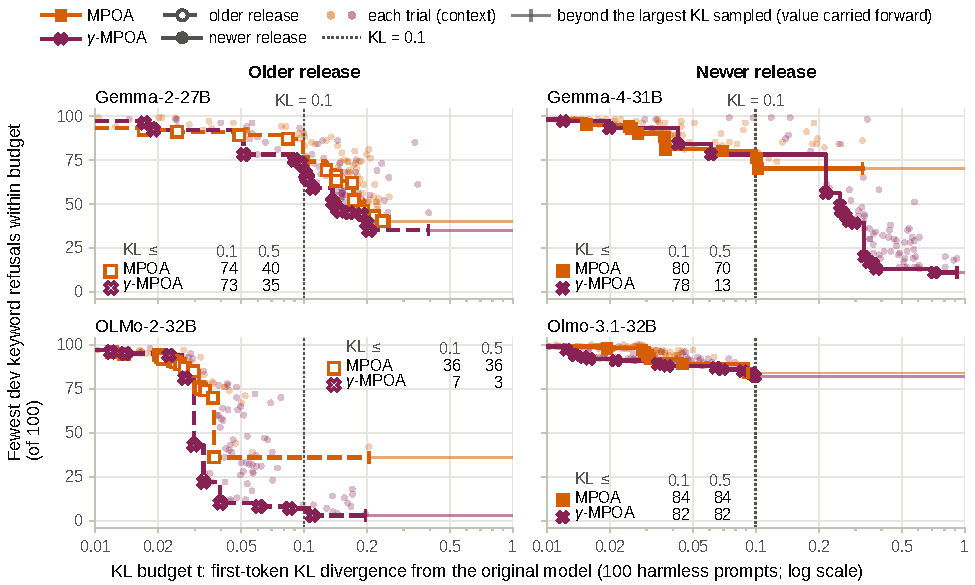
\includegraphics[width=\textwidth]{figures/fig9_gamma_mpoa.pdf}
\caption{\textbf{Gamma-corrected MPOA versus MPOA on the post-norm models (dev set).} One panel per model (columns: older and newer release; rows: Gemma, OLMo). A curve gives, for every KL budget $t$, the fewest dev keyword refusals (of 100) among the completed TPE trials of one run (100 trials, seed 1) with first-token KL divergence from the original at most $t$; it steps down at the run's Pareto-front trials (method markers; older release dashed and hollow, newer solid and filled). Past the largest KL sampled (end tick) the value is only carried forward (thin line). Faint dots: all completed trials; dotted line: the selection budget KL = 0.1; the small table (upper right for OLMo-2-32B, lower left elsewhere) reads each curve at KL $\le$ 0.1 and $\le$ 0.5. MPOA vs $\gamma$-MPOA: on Gemma-2-27B the correction changes little (74 vs 73 at KL $\le$ 0.1, 40 vs 35 at KL $\le$ 0.5). On Gemma-4-31B the two are close at KL $\le$ 0.1 (80 vs 78) but separate at larger budgets (70 vs 13 at KL $\le$ 0.5), a gap confounded with search coverage (MPOA placed 14 of 100 trials above KL 0.1, $\gamma$-MPOA 82): the MPOA curve is flat there because that region was barely explored, not because lower counts were shown to be unreachable. On OLMo-2-32B the correction lowers the count at the selection budget itself (36 vs 7 at KL $\le$ 0.1, 36 vs 3 at KL $\le$ 0.5), with similar search coverage (99 and 88 of 100 trials at KL $\le$ 0.1, none above 0.3), so this gap is not a coverage artefact. On Olmo-3.1-32B the correction changes little (84 vs 82 at KL $\le$ 0.1; neither search sampled a larger KL, so the KL $\le$ 0.5 values only repeat these). All counts are dev keyword refusals on the 100 prompts also used for optimisation and selection, not held-out refusal rates; one search per run (seed 1), budgets other than 0.1 read post hoc.}
\label{fig:gmpoa-dev}
\end{figure*}
% caption: paper/figures/captions.md (fig9_gamma_mpoa)


\paragraph{Community releases.} Of eight public abliterations
(Figures~\ref{fig:community} and~\ref{fig:community-releases}), four refused
less than the best model selected here for the same checkpoint (all
$p_\mathrm{Holm}<0.001$), for example on Qwen3.8-27B (1.4\% [0.9, 2.4] vs.\
14.0\% [12.0, 16.3]; $-$12.6~pp [$-$14.8, $-$10.5]); two did not differ significantly and two refused more. The
four had teacher-forced divergences of 0.085--0.151 (best selected models
0.042--0.060) and mean capability changes of $-$0.94 to $-$0.15~pp. On three
of the five checkpoints with a public release (Qwen2.5-32B, Qwen3.8-27B,
Olmo-3.1-32B), a public release refused less than every model selected here
under the KL cap; on the other two (Gemma-4-31B, Mistral-Small-3.2) the best
release did not differ significantly from the best selected model.
% src: results/analysis/final_community_vs_selected.csv (p_holm_within_community; Holm over 4 per release)
% src (review revision): final_community_vs_selected.csv rows with ours_is_best_wg: qwen2.5-32b huihui 1.3% / zetasepic 1.1% vs
% src: mpoa 3.9%, qwen3.8-27b huihui 1.4% vs mpoa 14.0%, olmo-3.1-32b muxodious 0.7% vs ara 10.8% (all p_holm < 0.001);
% src: gemma-4-31b coder3101 0.9% vs ara 0.6% (p_holm 0.51); mistral-small-3.2 huihui 5.0% vs mpoa 4.0% (p_holm 0.44);
% src: "3 of the 5 checkpoints" = paper/figures/captions.md (fig14_community), moved from the caption.


\paragraph{Seed sensitivity.} On the small pair a second seed changed the
selected dev count by a median of 8 and up to 35 refusals
(Figure~\ref{fig:seed-dev}), and held-out refusal differed between seeds in
all 10 cells after Holm correction (median 9.4~pp, maximum 25.2~pp;
item-level $\kappa=0.08$--0.79; Figure~\ref{fig:seed-heldout}); these
differences give the run-to-run standard deviation used in
\S\ref{sec:res-h1}. The ARA
generation effect was +14.2~pp with seed~1 and +0.0~pp [$-$1.2, +1.2]
($p=1.00$) with seed~2, the direction-based effects changed from +34.1, +4.2,
+9.7 and +21.2~pp (DiM, MPOA, SOM, J-space) to +44.3, +30.1, +29.6 and
+10.6~pp, and the H2 risk-difference contrast was $-$3.1~pp with seed~1 and
$-$28.7~pp [$-$31.0, $-$26.5] with seed~2. Method accounted for $\eta^2=0.94$ and 0.88
of the variance among the ten cell rates of Qwen2.5-7B and Qwen3.5-4B
($F(4,5)=19.46$ and 9.58, $p=0.003$ and 0.015).
% src: paper/figures/captions.md (fig8 "For the text": |s1 - s2| median 8, max 35); results/analysis/final_seed_cells.csv;
% src: final_seed_generation.csv; final_seed_method_vs_seed.csv (eta_sq_method, anova_F, anova_p); seed-2 per-method
% src: generation effects (DiM +44.3, MPOA +30.1, SOM +29.6, J-space +10.6) moved from the fig13 caption (paper/figures/captions.md,
% src: fig13_seed_heldout; final_seed_generation.csv) in the review revision.

\begin{figure*}[!htbp]
\centering
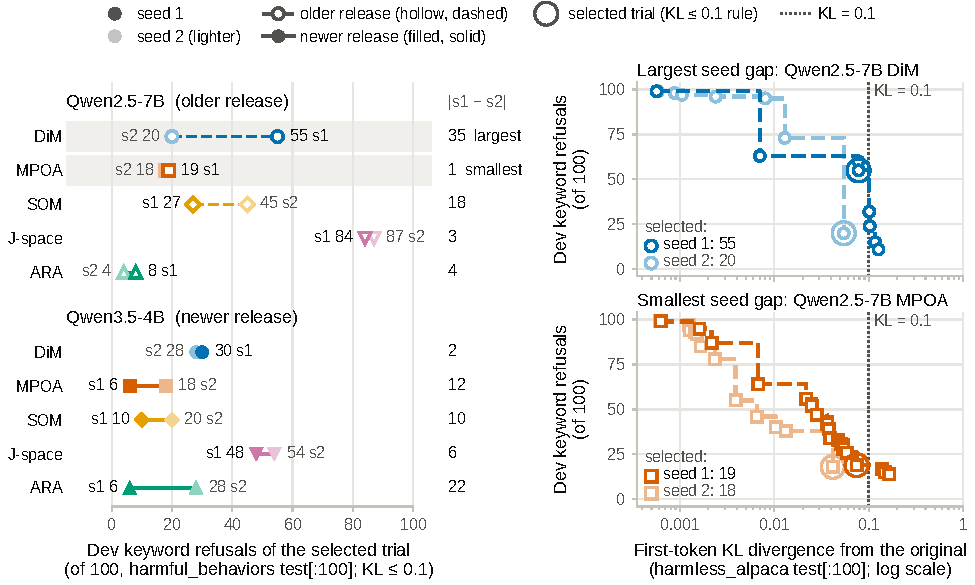
\includegraphics[width=\textwidth]{figures/fig8_seed_sensitivity.pdf}
\caption{\textbf{Seed sensitivity of the selected trial (dev set, small pair).} Each row is one model $\times$ method cell of the small Qwen pair, optimised twice with 100 TPE trials that differ only in the seed (same configuration, Heretic commit and RTX 4090). The two markers give the dev keyword refusals (of 100) of the trial chosen by the selection rule (fewest dev keyword refusals at first-token KL $\le$ 0.1) in the seed-1 run (full colour) and the seed-2 run (lighter); the column on the right is their absolute difference. Hollow markers and dashed lines mark the older model (Qwen2.5-7B), filled markers and solid lines the newer one (Qwen3.5-4B). The right panels show both seeds' Pareto fronts for the cell with the largest difference (Qwen2.5-7B DiM, 55 vs 20) and the cell with the smallest (Qwen2.5-7B MPOA, 19 vs 18). In the fronts, the rings mark each seed's selected trial and the dotted line the KL = 0.1 threshold. All counts are keyword matches on the 100 dev prompts used for optimisation and selection, not held-out refusal rates; seed 1 is the run evaluated elsewhere in the paper.}
\label{fig:seed-dev}
\end{figure*}
% caption: paper/figures/captions.md (fig8_seed_sensitivity)


\paragraph{Over-refusal.} WildGuard refusal on the 350 benign held-out prompts
fell from 4.3--22.3\% in the originals to 0.0--7.4\% in the 42 primary models,
significantly in 41 of them (exact McNemar, Holm over all 64 modified models);
only Gemma-4-31B DiM, the failed edit, did not change significantly (+1.1~pp,
$p_\mathrm{Holm}=0.250$).
% src: results/analysis/secondary_overrefusal.csv (item_group benign_all; wg_overrefusal_rate originals 0.043 qwen2.5-7b to 0.223 gemma-2-27b; primary 0.000 to 0.074 gemma-2-27b__som 26/350; wg_mcnemar_p_holm < 0.05 with wg_delta_pp < 0 in 41 of 42 primary; gemma-4-31b__dim +1.14 pp, p 0.125, p_holm 0.250; Holm over the 64 modified cells)

\paragraph{Harmful compliance.} Residual refusal is not the same as harmful
compliance. Of the ablated main-study responses that WildGuard did not label
as refusals, 75.1\% [73.4, 76.9] were harmful according to the HarmBench
classifier and 55.8\% [53.3, 58.1] according to WildGuard's harmful-response
label (all ten originals: 79.0\% and 29.6\%), so 16.8\% [15.7, 18.0] of all ablated
main-study responses were neither refused nor harmful by HarmBench. With
harmful compliance as the outcome, coded as not harmful so that a positive
generation effect again means that removal left less on the newer model, the
pooled conclusions were the same (Appendix~\ref{app:harm}). The
baseline-adjusted direction-based effect was +0.05 log-odds [$-$0.02, +0.11]
(HarmBench) and $-$0.03 [$-$0.13, +0.07] (WildGuard), against +0.03 for
refusal; the H2 interaction was $-$0.49 [$-$0.56, $-$0.41] and $-$0.45
[$-$0.52, $-$0.38], against $-$0.50; and per pair the interaction was in the
predicted direction for Gemma and OLMo and opposite for Qwen under every
outcome. Several per-pair results changed. Under HarmBench every Qwen method
was significantly higher on the newer model, so the Qwen pair met the H1
criterion on this outcome: Qwen SOM, Gemma MPOA and Gemma SOM became
significantly higher, Mistral Small DiM lost significance and Mistral Small
ARA became significantly lower. The raw pooled ARA effect became significant
(+0.21 [+0.14, +0.28] and +0.24 [+0.18, +0.30], against +0.12 for refusal),
and the Holm tally of the 16 main-pair tests was 11 higher, 3 lower and 2 not
significant (HarmBench) and 10, 1 and 5 (WildGuard), against 8, 4 and 4.
% src (review revision): results/analysis/review_out_c3_pooled.csv (ablated, main study (32): HB harmful among not refused
% src: 75.1 [73.4, 76.9], WG harmful among not refused 55.8 [53.3, 58.1], not refused and not HB-harmful 16.8 [15.7, 18.0];
% src: originals 79.0 / 29.6) = review_out_summary.md C3 "How much of 'not refused'"; review_out_c3_models.csv (hbnc / wghnc,
% src: main: gee_with_originals direction +0.05 [-0.02, +0.11] / -0.03 [-0.13, +0.07]; gee_planned gen_new:opt -0.49 [-0.56,
% src: -0.41] / -0.45 [-0.52, -0.38]; optimisation class +0.21 [+0.14, +0.28] / +0.24 [+0.18, +0.30]); review_out_c3_tests.csv
% src: (H1 tallies 11/3/2 and 10/1/5; changed Holm decisions listed in review_out_summary.md C3); review_out_c3_h2_contrasts.csv
% src: (per-pair interactions: gemma, olmo negative and qwen positive under every outcome).

\paragraph{Capability and divergence.} Across the 42 primary models, mean
capability change ranged from $-$4.2~pp (OLMo-2-32B ARA) to +0.9~pp
(Qwen2.5-7B J-space; Figure~\ref{fig:capability},
Tables~\ref{tab:capability-main}--\ref{tab:capability-small}), and
teacher-forced divergence from 0.004 to 0.279 nats per token
(Figure~\ref{fig:divergence},
Tables~\ref{tab:teacher-forced-main}--\ref{tab:teacher-forced-small}). Across
the 56 modified models with a dev trial, capability change was not correlated
with selected dev KL (Spearman $\rho=-0.03$ [$-$0.29, +0.24], $p=0.81$) but
was with teacher-forced divergence ($\rho=-0.48$ [$-$0.66, $-$0.24],
$p<0.001$); every selected trial had KL~$\le 0.1$ by design. Among the 42
primary models alone, the correlations were $\rho=+0.08$ [$-$0.22, +0.38]
($p=0.63$) with dev KL and $-0.39$ [$-$0.63, $-$0.11] ($p=0.010$) with
teacher-forced divergence.
% src: results/analysis/final_kl_vs_capability_cells.csv (role primary); paper/tables/t3_teacher_forced.csv;
% src: paper/figures/captions.md (fig6 range); final_kl_vs_capability.csv (n = 56; "primary seed 1 only" rows, n = 42)



\paragraph{Development set versus held-out refusal.} On the dev prompts used
for search and selection (Figures~\ref{fig:pareto}--\ref{fig:kl-budget},
Table~\ref{tab:dev-refusals-main}), the selected keyword count changed from
older to newer model by $-$2.8 (DiM), +17.3
(MPOA), +20.3 (ARA) and $-$4.5 (SOM) refusals on average over the main pairs
(Figure~\ref{fig:dev-generation}). The newer models' ARA counts (Qwen, Gemma,
OLMo, Mistral Small) were 63, 28, 48 and 6 at a KL budget of 0.1 and 21, 9, 34
and 6 at 0.2 (Figure~\ref{fig:kl-budget}). Gemma-4-31B ARA, with 28 dev
keyword refusals, had 22.3\% [19.8, 25.0] held-out keyword refusals and 0.6\%
held-out WildGuard refusals. Dev refusals correlated with held-out refusal
across the 42 primary models ($\rho=0.77$ [0.61, 0.87]; older models 0.85,
newer 0.73), and the best dev method was the
best held-out method in 7 of 12 model $\times$ seed sets (6 of 12 without the
KL tie-break).
The direction of the change could differ between the two sets: in 3 of the 16
main-pair method cells (Qwen DiM, Gemma ARA, Mistral Small MPOA) the dev change
and a significant held-out change had opposite signs, and on the small pair
every method's dev count fell from the older to the newer model while every
held-out rate rose (Figure~\ref{fig:dev-generation}).
% src: paper/tables/t1_dev_refusals_main.tex; paper/figures/captions.md (fig3 "For the text" means);
% src: results/analysis/final_log.txt (d); final_dev_vs_heldout_within_model.csv;
% src: h1h2_cells.csv (gemma-4-31b__ara: kw 217/972 = 0.2233 [0.1982, 0.2505]; wg 6/972 = 0.0062)

\paragraph{Re-scoring the released exports.} The 46 released merged exports were
re-scored on the development set with Heretic's own evaluator. Their keyword
refusal counts were within two of the selected trials' counts for 37 of 46
(median change +1, range $-$7 to +9, largest for ARA), first-token KL changed
by a median of +0.0003, and four exports (Gemma-2-27B MPOA, Gemma-4-31B ARA
and the $\gamma$-MPOA controls of Gemma-2-27B and Olmo-3.1-32B) re-scored
slightly above the KL budget, at 0.103 to 0.107
(Appendix~\ref{app:dev-rescore}). The largest changes were in ARA exports
whose adapter had been refitted on a different GPU from the search
(\S\ref{sec:res-h2}). The re-score also showed that the five
Gemma-2-27B exports had been saved without the eager-attention setting that
transformers needs for Gemma-2's attention-logit soft-capping; their public
configurations were patched, and the held-out results are unaffected because
all generations, benchmarks and teacher-forced divergences were computed in
vLLM, which applies the soft-cap from the configuration regardless of this
setting.
% src (2026-11-06, integration): results/analysis/dev_rescore_groups.csv (row "all 46 released exports": n_within_2 37,
% src: median_d_ref 1, min_d_ref -7, max_d_ref 9, median_d_kl 0.0003, n_over_kl_cap 4); results/analysis/dev_rescore_cells.csv
% src: (d_refusals +9 qwen3.8-27b ara and -7 gemma-4-31b ara; over_kl_cap rows: gemma-2-27b mpoa 0.1036, gemma-4-31b ara
% src: 0.1070, gemma-2-27b gmpoa 0.1059, olmo-3.1-32b gmpoa 0.1032; gemma2_eager rows: evaluated_rev, patched_rev12);
% src: notes/gemma2_config_patch_20261106.log; details, mechanism and vLLM check in sections/08f_dev_rescore.tex (app:dev-rescore)
% src (review revision): results/analysis/review_sel_export_drift.csv, review_sel_export_tests.csv (ARA, other machine 4/4 drift > 2)


\begin{figure*}[!htbp]
\centering
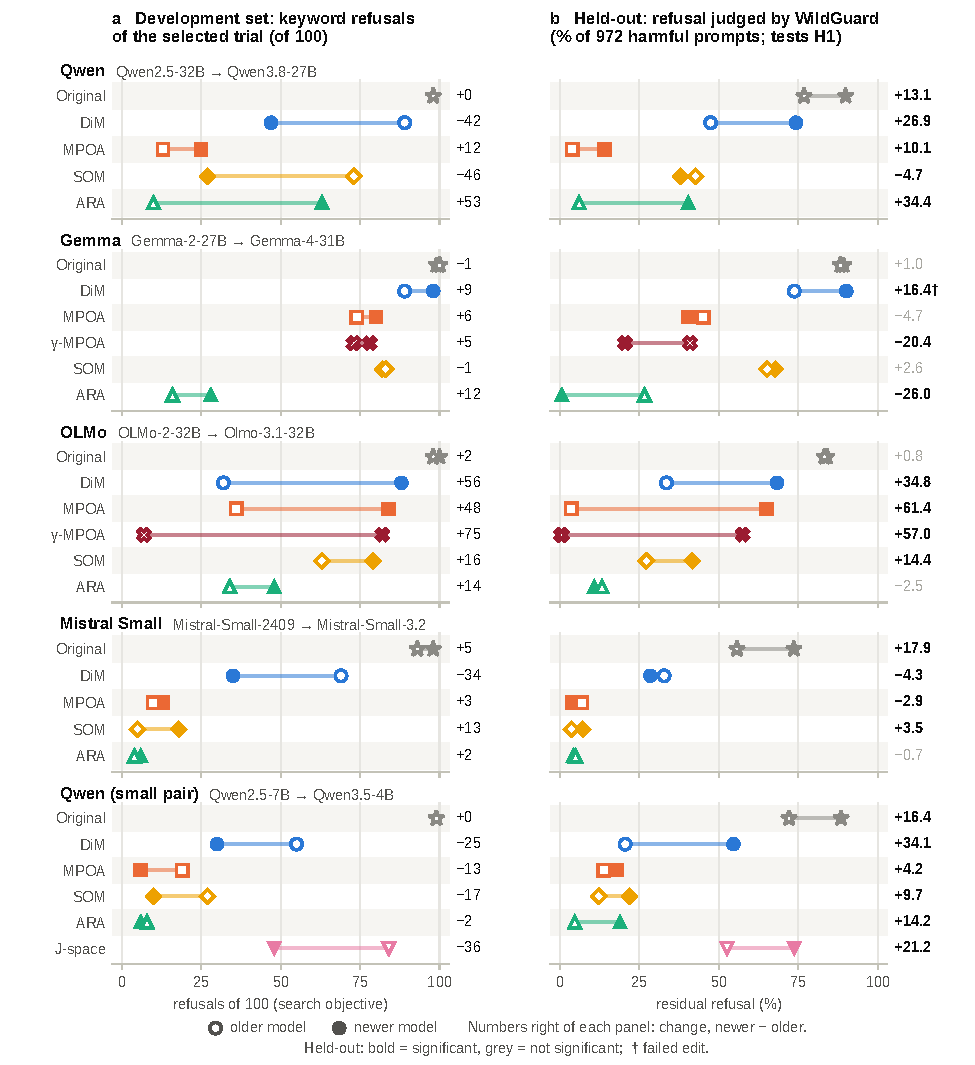
\includegraphics[width=\textwidth]{figures/fig3v_generation_dev_heldout.pdf}
\caption{\textbf{Generation effect on the development set (a) and on held-out prompts (b).} One block per pair, one row per condition; hollow = older, filled = newer model; the number right of each panel is the change, newer $-$ older. (a) Dev keyword refusals (of 100) of the trial picked by the selection rule (fewest dev refusals at first-token KL $\le$ 0.1, seed 1); the Original row gives the unedited models. These prompts were also used for search and selection, so the counts are optimistically biased and untested; seed-to-seed variation is shown in Figure~\ref{fig:seed-dev}. (b) Held-out refusal judged by WildGuard, paired over the 972 harmful prompts: the H1 measure, with the same values as Figure~\ref{fig:heldout-generation} and Table~\ref{tab:h1-heldout}. Bold: significant; grey: not significant. Significance for the methods is Holm-adjusted (exact McNemar, Holm within the 23 H1 tests); significance for the originals and $\gamma$-MPOA is unadjusted (exact McNemar), because they are not H1 tests; $\dagger$ failed edit (held-out refusal not below the model's own original). $\gamma$-MPOA was run on the Gemma and OLMo pairs only, J-space on the small pair only. Single seed; 95\% Wilson intervals for (b) are in Figure~\ref{fig:heldout-generation}.}
\label{fig:dev-generation}
\end{figure*}
% caption: paper/figures/captions.md (fig3v_generation_dev_heldout); replaces the horizontal fig3_generation_effect (user request 2026-11-05)
% review revision 2026-11-06 (minor m2): the significance sentence states explicitly which markers are Holm-adjusted.

\begin{figure*}[!htbp]
\centering
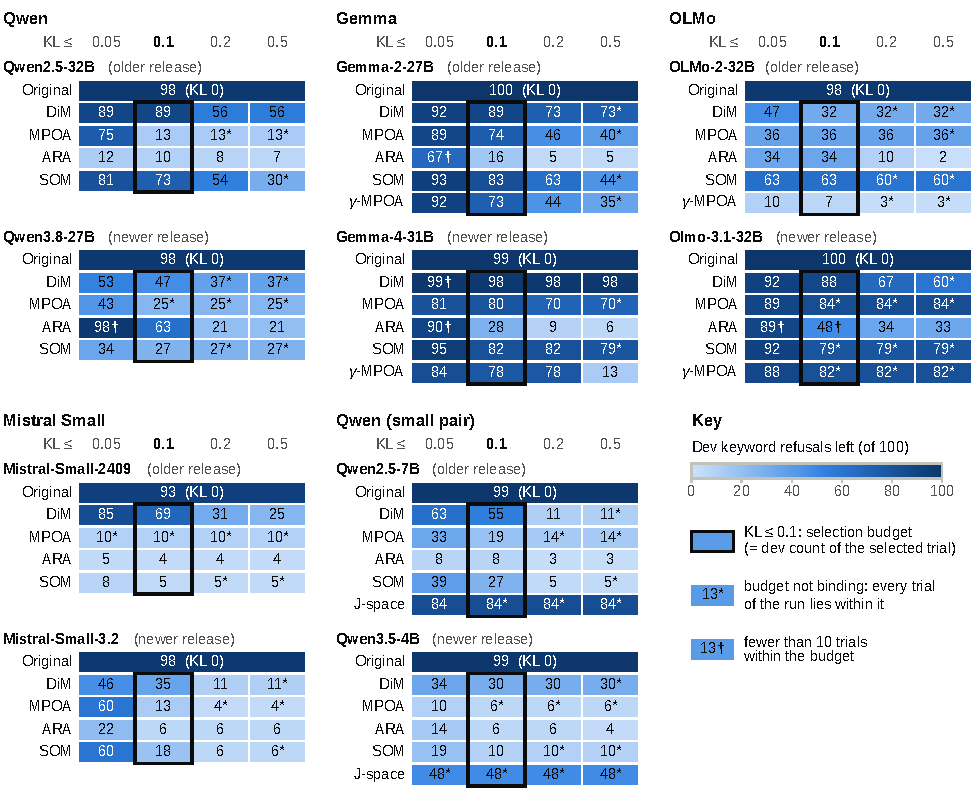
\includegraphics[width=\textwidth]{figures/fig4_kl_budget_heatmap.pdf}
\caption{\textbf{How much refusal is left at a given KL budget (dev set).} Each cell is the fewest dev keyword refusals (of 100) among the completed TPE trials of one optimisation run whose first-token KL divergence from the original is at most the column budget $t$. Within each pair the upper block is the older and the lower block the newer release; each block starts with the unedited original (KL 0). Darker cells mean more refusal survives. The outlined $t = 0.1$ column is the selection budget, so it equals the dev refusals of the selected models. A degree sign ($^\circ$) marks a budget that is not binding (60 cells: every completed trial already lies within it, so larger budgets were never explored and the value is the run's overall minimum); a dagger marks a minimum over fewer than 10 trials (6 cells). The columns are post-hoc budgets on one 100-trial search per run (seed 1), not separate optimisations, and the counts are dev-set numbers, not held-out refusal rates.}
\label{fig:kl-budget}
\end{figure*}
% caption: paper/figures/captions.md (fig4_kl_budget_heatmap)

\paragraph{Search convergence.} Of the 42 core runs, 34 reached their
selected count by trial 75 (median trial 48) and 8 (19\%) improved later, by
1--14 refusals (Figures~\ref{fig:search-convergence}
and~\ref{fig:search-runs}); late runs were equally frequent on older and newer
models (4 of 21 each; Fisher $p=1.0$). The failed Gemma-4-31B DiM run
reached its selected count (98) at trial 40.
% src: results/analysis/final_search_runs.csv, final_search_tests.csv; paper/figures/captions.md (fig7)

\begin{figure*}[!htbp]
\centering
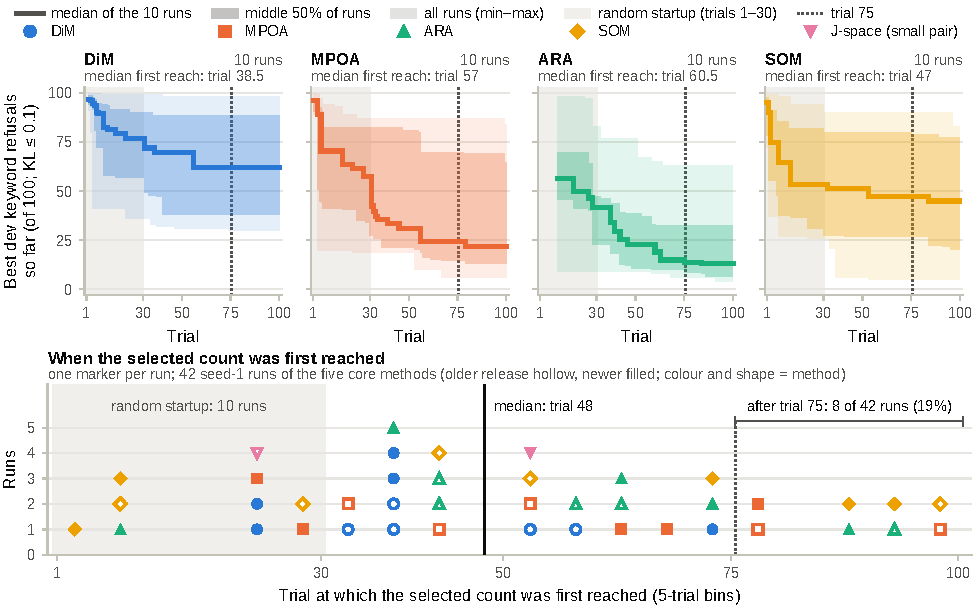
\includegraphics[width=\textwidth]{figures/fig7_search_convergence.pdf}
\caption{\textbf{Search-budget convergence of the 100-trial TPE searches (dev set).} Top: for each core method with ten runs (seed 1; five pairs, older and newer release), the median over the runs of the best count so far: after trial $t$, the fewest dev keyword refusals (of 100) among trials 1 to $t$ with first-token KL divergence $\le$ 0.1 from the original, i.e. the count the selection rule would have returned had the search stopped at trial $t$. Dark band: middle 50\% of the runs (25th--75th percentile); light band: all runs (minimum to maximum). Curves start at the run's first trial within the KL budget (trials 5--10 for ARA, 1--2 otherwise); the median and bands start once every run has a value. The grey band marks the 30 random startup trials of the TPE sampler, the dotted line trial 75. Bottom: the trial at which each of the 42 core runs (DiM, MPOA, ARA, SOM and, on the small pair, J-space) first reached the count it finally selected (median 48; 10 runs within the random startup); hollow markers are older, filled markers newer releases, colour and shape the method. The 8 runs (19\%) that still improved after trial 75, by 1--14 refusals, show that the selected counts are not converged minima; for the other 34 runs these data cannot tell whether a longer search would have helped. Every run is drawn as its own curve, by method and release, in Figure~\ref{fig:search-runs}, together with the two J-space runs and the 4 $\gamma$-MPOA runs (Gemma and OLMo pairs only; not counted in the histogram). All counts are keyword matches on the 100 dev prompts that were also used for search and selection, not held-out refusal rates.}
\label{fig:search-convergence}
\end{figure*}
% caption: paper/figures/captions.md (fig7_search_convergence)



\clearpage
% ------------------------------------------------------------
\subsection{Run-to-Run Variance as a Function of the Refusal Level}
\label{app:sigma-level}

The per-pair intervals of Table~\ref{tab:pair-effects} add a run-to-run
variance $\sigma^2$ per optimised cell, with $\sigma=9.15$~pp [6.40, 16.07]
estimated from the ten small-pair seed pairs and assumed constant across
models, methods and refusal levels (\S\ref{sec:setup-stats}). A binomial-type
rate varies less near 0\% and 100\%, so a second model holds the run effect
constant on the logit scale, $\sigma_L=0.83$ [0.58, 1.45] from the same seed
pairs, and maps it to percentage points at each cell's observed rate $p$ by
the delta method, $\sigma_{\mathrm{pp}}=\sigma_L\,p(1-p)$. This gives about
0.5~pp for Gemma-4-31B ARA (0.6\% refusal) and up to 20.7~pp at 50\% refusal.
The ten seed pairs do not distinguish the two models (log-likelihood of the
pp differences 6.25 under the constant model and 6.01 under the logit model;
rank correlation between $|d|$ and $\bar p(1-\bar p)$ $-0.01$). Under the
logit model, 1 of the 16 main-study per-method effects (OLMo MPOA) exceeded
twice the run-to-run standard deviation of a difference, against 5 under the
constant model; across the 95\% interval of $\sigma_L$, 0 to 3 did. Per pair
(Table~\ref{tab:sigma-level}), the OLMo direction-based increase excluded zero
under both models except at the upper limit of the logit model, whereas the
Qwen ARA increase, the Gemma ARA decrease and the Gemma H2 contrast excluded
zero only under the constant model. Table~\ref{tab:heterogeneity} gives the
between-pair heterogeneity with each kind of within-pair variance, including
the between-pair variance $\tau^2$ of every estimand, and
Table~\ref{tab:pair-variances} the within-pair variances used as weights. The
headline $I^2$ of the raw direction-based pp effect is therefore 80\% only
under the constant variance model at the point estimate of $\sigma$; under
the refusal-level model it is 46\% ($\tau^2=127$~pp$^2$ against 225~pp$^2$).
% 2026-11-08 ARS re-review revision (REV-14, NEW-3): t11 replaced by t11b (same Q, p, I2, plus tau2) and t14 added
% (scripts/analysis/revision_rr_extra.py from revision_heterogeneity.csv and revision_pair_variances.csv).
% src: results/analysis/revision_sigma_model.csv (sigma_pp 9.154 [6.396, 16.065]; sigma_L 0.828 [0.578, 1.453]; log-likelihood 6.254 /
% src: 6.007; Spearman -0.006); revision_sigma_cells.csv (gemma-4-31b ara sigma_level_pp_point 0.51); 0.828 x 0.25 = 20.7 pp;
% src: revision_sigma_method_flags.csv (exceeds_level lo / point / hi: 3 / 1 / 0; exceeds_const point 5);
% src: revision_sigma_pair_verdicts.csv; revision_heterogeneity.csv; revision_pair_variances.csv
% src: (all written by scripts/analysis/revision_seed_variance.py, 2026-11-08).

% Auto-generated by scripts/analysis/revision_make_tables.py at 2026-11-09T00:34Z -- do not edit by hand.
% src: results/analysis/revision_sigma_pair_verdicts.csv (scripts/analysis/revision_seed_variance.py)
\begin{table*}[t]
\centering\scriptsize
\setlength{\tabcolsep}{3pt}
\caption{Per-pair class effects (pp) under two models of run-to-run variance. Constant: $\sigma=9.15$~pp per cell [6.40, 16.07] (the intervals of Table~\ref{tab:pair-effects}). Refusal-level: $\sigma_L=0.83$ [0.58, 1.45] per cell on the logit scale, mapped to pp at each cell's rate $p$ as $\sigma_L\,p(1-p)$. Intervals add prompt sampling and the run-to-run variance at the point estimate of $\sigma$; the last two columns mark (\checkmark) whether the interval excludes zero at the lower limit, point estimate and upper limit of $\sigma$ (lo\,/\,pt\,/\,hi).}
\label{tab:sigma-level}
\begin{tabular}{@{}lllllcc@{}}
\toprule
Pair & Estimand & Effect & Constant $\sigma$ & Refusal-level $\sigma$ & Excl.\ 0, const. & Excl.\ 0, level \\
 & & & [95\% interval] & [95\% interval] & lo/pt/hi & lo/pt/hi \\
\midrule
Qwen & Direction, raw & +10.7 & [$-$4.0, +25.5] & [$-$15.3, +36.7] & \checkmark/--/-- & --/--/-- \\
 & Direction, adjusted & $-$2.4 & [$-$17.3, +12.5] & [$-$28.5, +23.7] & --/--/-- & --/--/-- \\
 & ARA, raw & +34.4 & [+8.8, +59.9] & [$-$5.9, +74.6] & \checkmark/\checkmark/-- & \checkmark/--/-- \\
 & ARA, adjusted & +21.3 & [$-$4.4, +47.0] & [$-$19.0, +61.7] & \checkmark/--/-- & --/--/-- \\
 & H2 contrast & +23.6 & [$-$5.9, +53.1] & [$-$24.3, +71.6] & \checkmark/--/-- & --/--/-- \\
\addlinespace
Gemma & Direction, raw & +4.7 & [$-$10.2, +19.6] & [$-$23.2, +32.6] & --/--/-- & --/--/-- \\
 & Direction, adjusted & +3.7 & [$-$11.2, +18.6] & [$-$24.2, +31.6] & --/--/-- & --/--/-- \\
 & ARA, raw & $-$26.0 & [$-$51.6, $-$0.5] & [$-$57.9, +5.8] & \checkmark/\checkmark/-- & \checkmark/--/-- \\
 & ARA, adjusted & $-$27.1 & [$-$52.7, $-$1.5] & [$-$59.0, +4.9] & \checkmark/\checkmark/-- & \checkmark/--/-- \\
 & H2 contrast & $-$30.8 & [$-$60.2, $-$1.3] & [$-$73.1, +11.5] & \checkmark/\checkmark/-- & \checkmark/--/-- \\
\addlinespace
OLMo & Direction, raw & +36.9 & [+22.1, +51.7] & [+9.8, +63.9] & \checkmark/\checkmark/\checkmark & \checkmark/\checkmark/-- \\
 & Direction, adjusted & +36.0 & [+21.2, +50.9] & [+9.0, +63.1] & \checkmark/\checkmark/\checkmark & \checkmark/\checkmark/-- \\
 & ARA, raw & $-$2.5 & [$-$27.9, +23.0] & [$-$26.9, +22.0] & --/--/-- & --/--/-- \\
 & ARA, adjusted & $-$3.3 & [$-$28.8, +22.2] & [$-$27.8, +21.2] & --/--/-- & --/--/-- \\
 & H2 contrast & $-$39.3 & [$-$68.8, $-$9.9] & [$-$75.8, $-$2.9] & \checkmark/\checkmark/-- & \checkmark/\checkmark/-- \\
\addlinespace
Mistral Small & Direction, raw & $-$1.2 & [$-$16.0, +13.5] & [$-$18.5, +16.1] & --/--/-- & --/--/-- \\
 & Direction, adjusted & $-$19.2 & [$-$34.1, $-$4.2] & [$-$36.6, $-$1.7] & \checkmark/\checkmark/-- & \checkmark/\checkmark/-- \\
 & ARA, raw & $-$0.7 & [$-$26.1, +24.7] & [$-$10.8, +9.4] & --/--/-- & --/--/-- \\
 & ARA, adjusted & $-$18.6 & [$-$44.2, +6.9] & [$-$29.1, $-$8.2] & \checkmark/--/-- & \checkmark/\checkmark/\checkmark \\
 & H2 contrast & +0.5 & [$-$28.8, +29.9] & [$-$19.5, +20.5] & --/--/-- & --/--/-- \\
\addlinespace
Small pair & Direction, raw & +17.3 & [+4.4, +30.1] & [$-$3.7, +38.2] & \checkmark/\checkmark/-- & \checkmark/--/-- \\
 & Direction, adjusted & +0.9 & [$-$12.1, +14.0] & [$-$20.2, +22.0] & --/--/-- & --/--/-- \\
 & ARA, raw & +14.2 & [$-$11.3, +39.7] & [$-$11.9, +40.3] & --/--/-- & --/--/-- \\
 & ARA, adjusted & $-$2.2 & [$-$27.8, +23.5] & [$-$28.4, +24.1] & --/--/-- & --/--/-- \\
 & H2 contrast & $-$3.1 & [$-$31.6, +25.4] & [$-$36.5, +30.3] & --/--/-- & --/--/-- \\
\bottomrule
\end{tabular}
\end{table*}

% Auto-generated by scripts/analysis/revision_rr_extra.py at 2026-11-09T04:36Z -- do not edit by hand.
% src: results/analysis/revision_heterogeneity.csv (scripts/analysis/revision_seed_variance.py); tau^2 in pp^2
% (pp scale, tau2 x 10^4) and log-odds^2. Same Q, p and I^2 as t11_heterogeneity.tex, with tau^2 added.
\begin{table}[t]
\centering\scriptsize
\setlength{\tabcolsep}{2pt}
\caption{Between-pair heterogeneity of the four main-pair effects with three kinds of within-pair variance: prompt sampling only, prompt sampling plus constant run-to-run variance, and (pp scale only) prompt sampling plus refusal-level run-to-run variance, each at the point estimate of $\sigma$. Each cell gives Cochran's $Q$ (3~df); its $p$ value; $I^2$; and the DerSimonian--Laird between-pair variance $\tau^2$ (pp$^2$ on the pp scale, squared log-odds on the log-odds scale). Across the 95\% interval of $\sigma$, $I^2$ of the raw direction-based pp effect is 90\% (lower limit) to 39\% (upper limit) with constant and 73\% to 0\% with refusal-level variance. The within-pair variances are in Table~\ref{tab:pair-variances}.}
\label{tab:heterogeneity}
\begin{tabular}{@{}lccccc@{}}
\toprule
 & \multicolumn{3}{c}{pp scale} & \multicolumn{2}{c}{log-odds scale} \\
\cmidrule(lr){2-4}\cmidrule(l){5-6}
Estimand & Prompt only & + seed, const. & + seed, level & Prompt only & + seed \\
\midrule
Direction, raw & 821.8; $<$0.001; 100\%; 284 & 14.8; 0.002; 80\%; 225 & 5.5; 0.136; 46\%; 127 & 590.8; $<$0.001; 99\%; 0.56 & 3.8; 0.289; 20\%; 0.12 \\
Direction, adjusted & 849.4; $<$0.001; 100\%; 527 & 27.7; $<$0.001; 89\%; 476 & 11.5; 0.010; 74\%; 425 & 608.6; $<$0.001; 100\%; 1.53 & 7.7; 0.053; 61\%; 0.72 \\
ARA, raw & 807.1; $<$0.001; 100\%; 321 & 10.9; 0.012; 73\%; 447 & 5.3; 0.148; 44\%; 113 & 378.5; $<$0.001; 99\%; 2.86 & 14.3; 0.003; 79\%; 5.34 \\
ARA, adjusted & 381.8; $<$0.001; 99\%; 328 & 7.9; 0.048; 62\%; 278 & 5.0; 0.172; 40\%; 97 & 208.5; $<$0.001; 99\%; 1.95 & 10.8; 0.013; 72\%; 3.74 \\
H2 contrast & 1006.7; $<$0.001; 100\%; 680 & 11.2; 0.011; 73\%; 614 & 6.3; 0.097; 53\%; 343 & 539.7; $<$0.001; 99\%; 4.54 & 10.8; 0.013; 72\%; 4.87 \\
\bottomrule
\end{tabular}
\end{table}

% Auto-generated by scripts/analysis/revision_rr_extra.py at 2026-11-09T04:36Z -- do not edit by hand.
% src: results/analysis/revision_pair_variances.csv (var_within; pp scale x 10^4 = pp^2)
\begin{table}[t]
\centering\scriptsize
\setlength{\tabcolsep}{3pt}
\caption{Within-pair variances of the four main-pair effects used as inverse-variance weights in Table~\ref{tab:heterogeneity}, at the point estimate of $\sigma$: prompt sampling only, and prompt sampling plus constant or refusal-level run-to-run variance. pp scale in pp$^2$; log-odds scale in squared log-odds. The constant run-to-run term is the same for every pair (2$\sigma^2$ per method, 2$\sigma^2/3$ for the direction-class mean), so on that variance model the pairs are weighted almost equally.}
\label{tab:pair-variances}
\begin{tabular}{@{}llrrrrr@{}}
\toprule
 & & \multicolumn{3}{c}{pp scale (pp$^2$)} & \multicolumn{2}{c}{log-odds scale} \\
\cmidrule(lr){3-5}\cmidrule(l){6-7}
Estimand & Pair & Prompt only & + seed, const. & + seed, level & Prompt only & + seed \\
\midrule
Direction, raw & Qwen & 1.0 & 56.8 & 176.0 & 0.002 & 0.459 \\
 & Gemma & 1.9 & 57.8 & 202.9 & 0.004 & 0.461 \\
 & OLMo & 1.2 & 57.1 & 190.0 & 0.003 & 0.459 \\
 & Mistral Small & 0.6 & 56.4 & 77.9 & 0.004 & 0.461 \\
\addlinespace
Direction, adjusted & Qwen & 1.9 & 57.8 & 177.0 & 0.009 & 0.466 \\
 & Gemma & 1.6 & 57.5 & 202.6 & 0.011 & 0.468 \\
 & OLMo & 1.7 & 57.5 & 190.5 & 0.005 & 0.462 \\
 & Mistral Small & 2.3 & 58.2 & 79.6 & 0.007 & 0.464 \\
\addlinespace
ARA, raw & Qwen & 2.6 & 170.2 & 422.4 & 0.019 & 1.389 \\
 & Gemma & 2.0 & 169.6 & 264.1 & 0.165 & 1.536 \\
 & OLMo & 1.2 & 168.8 & 155.6 & 0.010 & 1.381 \\
 & Mistral Small & 0.4 & 168.0 & 26.7 & 0.022 & 1.393 \\
\addlinespace
ARA, adjusted & Qwen & 4.3 & 171.9 & 424.1 & 0.025 & 1.396 \\
 & Gemma & 3.0 & 170.6 & 265.1 & 0.178 & 1.549 \\
 & OLMo & 1.6 & 169.2 & 156.1 & 0.013 & 1.384 \\
 & Mistral Small & 2.3 & 169.9 & 28.6 & 0.026 & 1.396 \\
\addlinespace
H2 contrast & Qwen & 3.3 & 226.7 & 598.2 & 0.019 & 1.847 \\
 & Gemma & 2.7 & 226.2 & 465.7 & 0.167 & 1.995 \\
 & OLMo & 2.3 & 225.7 & 345.5 & 0.012 & 1.840 \\
 & Mistral Small & 0.9 & 224.4 & 104.5 & 0.025 & 1.853 \\
\bottomrule
\end{tabular}
\end{table}


% ------------------------------------------------------------
\subsection{Verdicts at Other KL Budgets (Development Set)}
\label{app:kl-budgets}

Only the trial selected at first-token KL~$\le 0.1$ was evaluated on held-out
prompts, so other budgets can be read only on the 100 dev prompts, from the
completed trials of each search. For each run the refusal--KL front $f(t)$,
the fewest dev keyword refusals among trials with KL~$\le t$ (the original at
KL~$=0$ included), was read at $t=0.05$, 0.1, 0.2, 0.5 and 1.0, and summarised
without a budget as the area under the front, the mean of $f(t)$ over 200
log-spaced budgets between 0.01 and 1. Run-to-run variation of each quantity
was estimated from the ten small-pair seed pairs. In 7 of the 42 seed-1 runs
the front was carried forward beyond the largest sampled KL over more than
half of this range. Table~\ref{tab:kl-budgets} gives the class-level generation
effects. The direction-based effects kept their sign from KL~$\le 0.1$ to
KL~$\le 1.0$ in all four main pairs, and the OLMo direction-based increase
exceeded run-to-run variation at every budget and on the area. The dev ARA
effects had the same sign at every budget but the opposite sign to the
held-out ARA effects in three of the four main pairs, as at the selected
budget (\S\ref{sec:res-secondary}). The H2 contrast was positive at small
budgets and negative at large ones in Gemma, negative from KL~$\le 0.1$ on in
OLMo, and positive in Qwen at every budget.
% src: results/analysis/revision_kl_budget_runs.csv (carried_forward_share > 0.5 in 7 of 42 seed-1 runs; t0.1 equals the selected
% src: count in every run, checked in the script); revision_kl_budget_sigma.csv; revision_kl_budget_effects.csv (direction class
% src: sign_as_at_0.1 = 1 for t0.2 / t0.5 / t1 in all main pairs; olmo direction beyond_noise at every quantity; ara sign as held-out
% src: in 1 of 4 at every quantity; H2 gemma +22.7 / +7.3 / -18.7 / -29.0 / -29.0, olmo +12.7 / -26.0 / -10.0 / -0.7 / -27.7, qwen
% src: positive throughout) (scripts/analysis/revision_kl_budgets.py, 2026-11-08).

% Auto-generated by scripts/analysis/revision_make_tables.py at 2026-11-09T00:34Z -- do not edit by hand.
% src: results/analysis/revision_kl_budget_effects.csv, revision_kl_budget_sigma.csv (scripts/analysis/revision_kl_budgets.py; input paper/figures/data/trials.csv)
\begin{table*}[t]
\centering\scriptsize
\setlength{\tabcolsep}{3.5pt}
\caption{Generation effects on the development set at several first-token KL budgets (newer minus older model; dev keyword refusals of 100 of the best completed trial at KL $\le t$, including the original at KL = 0) and on the area under the refusal--KL front (mean front value over 200 log-spaced budgets from 0.01 to 1). Direction: mean of the direction-based methods; H2: ARA minus direction. $^{*}$Beyond 1.96 run-to-run standard errors, from the ten small-pair seed pairs on the same quantity (run-to-run SD per cell: $\le$0.05 6.8, $\le$0.1 10.8, $\le$0.2 5.2, $\le$0.5 4.6, $\le$1.0 4.6, Area 4.3; prompt sampling of the 100 dev prompts is not included). The KL $\le$ 0.1 column belongs to the selected models; only those were evaluated on held-out prompts (last column, WildGuard, pp). Dev counts are optimised and therefore optimistic.}
\label{tab:kl-budgets}
\begin{tabular}{@{}llrrrrrrr@{}}
\toprule
Pair & Estimand & $\le$0.05 & $\le$0.1 & $\le$0.2 & $\le$0.5 & $\le$1.0 & Area & Held-out \\
\midrule
Qwen & Direction & $-$38.3$^{*}$ & $-$25.3$^{*}$ & $-$11.3$^{*}$ & $-$3.3 & $-$3.3 & $-$7.2$^{*}$ & +10.7 \\
 & ARA & +86.0$^{*}$ & +53.0$^{*}$ & +13.0 & +14.0$^{*}$ & +1.0 & +37.1$^{*}$ & +34.4 \\
 & H2 contrast & +124.3$^{*}$ & +78.3$^{*}$ & +24.3$^{*}$ & +17.3$^{*}$ & +4.3 & +44.3$^{*}$ & +23.6 \\
\addlinespace
Gemma & Direction & +0.3 & +4.7 & +22.7$^{*}$ & +30.0$^{*}$ & +30.0$^{*}$ & +13.0$^{*}$ & +4.7 \\
 & ARA & +23.0$^{*}$ & +12.0 & +4.0 & +1.0 & +1.0 & +5.1 & $-$26.0 \\
 & H2 contrast & +22.7$^{*}$ & +7.3 & $-$18.7$^{*}$ & $-$29.0$^{*}$ & $-$29.0$^{*}$ & $-$7.9 & $-$30.8 \\
\addlinespace
OLMo & Direction & +42.3$^{*}$ & +40.0$^{*}$ & +34.0$^{*}$ & +31.7$^{*}$ & +31.7$^{*}$ & +27.9$^{*}$ & +36.9 \\
 & ARA & +55.0$^{*}$ & +14.0 & +24.0$^{*}$ & +31.0$^{*}$ & +4.0 & +21.9$^{*}$ & $-$2.5 \\
 & H2 contrast & +12.7 & $-$26.0 & $-$10.0 & $-$0.7 & $-$27.7$^{*}$ & $-$6.0 & $-$39.3 \\
\addlinespace
Mistral Small & Direction & +21.0$^{*}$ & $-$6.0 & $-$8.3 & $-$6.3 & $-$6.3 & +6.5 & $-$1.2 \\
 & ARA & +17.0 & +2.0 & +2.0 & +2.0 & +2.0 & +23.6$^{*}$ & $-$0.7 \\
 & H2 contrast & $-$4.0 & +8.0 & +10.3 & +8.3 & +8.3 & +17.1$^{*}$ & +0.5 \\
\addlinespace
Small pair & Direction & $-$27.0$^{*}$ & $-$22.8$^{*}$ & $-$5.0 & $-$5.0 & $-$5.0 & $-$11.6$^{*}$ & +17.3 \\
 & ARA & +6.0 & $-$2.0 & +3.0 & +1.0 & +1.0 & +4.0 & +14.2 \\
 & H2 contrast & +33.0$^{*}$ & +20.8 & +8.0 & +6.0 & +6.0 & +15.5$^{*}$ & $-$3.1 \\
\bottomrule
\end{tabular}
\end{table*}


% ------------------------------------------------------------
\subsection{Outcome Classes}
\label{app:outcome-classes}

Table~\ref{tab:outcome-classes} gives the four outcome classes of
\S\ref{sec:setup-eval} for every original and primary model. Degenerate
responses were at most 0.6\% of any of these models' responses. Among the 42 primary
models, incomplete compliance (generation stopped at the 512-token limit)
ranged from 7.6\% to 79.9\% of responses and complete compliance from 2.3\%
to 61.3\%; 65.8\% of all non-refused responses were incomplete. Incomplete
compliance is a property of the 512-token budget, not evidence that a
response was unhelpful.
% src: results/analysis/revision_outcome_classes_summary.md, revision_outcome_classes.csv (scripts/analysis/revision_outcome_classes.py,
% src: 2026-11-08; input cell_rates.csv harmful_all).

% Auto-generated by scripts/analysis/revision_make_tables.py at 2026-11-09T00:34Z -- do not edit by hand.
% src: results/analysis/revision_outcome_classes.csv (scripts/analysis/revision_outcome_classes.py; input cell_rates.csv, harmful_all)
\begin{table*}[t]
\centering\scriptsize
\setlength{\tabcolsep}{3.5pt}
\caption{Outcome classes on the 972 harmful held-out prompts (\% of responses), older and newer model of each pair: refusal (WildGuard, non-degenerate responses), complete compliance, incomplete compliance (generation stopped at the 512-token limit) and degenerate responses (Methods). Rows may not add to 100 because of rounding and a few unscored responses.}
\label{tab:outcome-classes}
\begin{tabular}{@{}llrrrrrrrr@{}}
\toprule
 & & \multicolumn{4}{c}{Older model} & \multicolumn{4}{c}{Newer model} \\
\cmidrule(lr){3-6}\cmidrule(l){7-10}
Pair & Condition & Ref. & Compl. & Incompl. & Degen. & Ref. & Compl. & Incompl. & Degen. \\
\midrule
Qwen & Original & 76.7 & 5.7 & 17.4 & 0.1 & 89.9 & 4.2 & 5.8 & 0.1 \\
 & DiM & 47.4 & 18.8 & 33.6 & 0.1 & 74.3 & 5.2 & 20.4 & 0.1 \\
 & MPOA & 3.9 & 50.6 & 45.4 & 0.1 & 14.0 & 8.7 & 77.3 & 0.0 \\
 & SOM & 42.7 & 20.4 & 36.8 & 0.1 & 38.0 & 14.0 & 47.8 & 0.2 \\
 & ARA & 6.1 & 61.3 & 32.5 & 0.1 & 40.3 & 4.5 & 54.9 & 0.2 \\
\addlinespace
Gemma & Original & 88.3 & 2.2 & 9.6 & 0.0 & 89.3 & 2.3 & 8.4 & 0.0 \\
 & DiM & 73.8 & 8.4 & 17.8 & 0.0 & 90.1 & 2.3 & 7.6 & 0.0 \\
 & MPOA & 45.2 & 27.1 & 27.8 & 0.0 & 40.4 & 11.0 & 48.6 & 0.0 \\
 & SOM & 65.2 & 13.6 & 21.2 & 0.0 & 67.7 & 9.9 & 22.3 & 0.1 \\
 & ARA & 26.6 & 46.1 & 27.3 & 0.0 & 0.6 & 19.4 & 79.9 & 0.0 \\
\addlinespace
OLMo & Original & 83.2 & 2.6 & 14.2 & 0.0 & 84.1 & 1.4 & 14.5 & 0.0 \\
 & DiM & 33.5 & 28.5 & 38.0 & 0.0 & 68.3 & 5.7 & 25.9 & 0.1 \\
 & MPOA & 3.6 & 42.0 & 54.4 & 0.0 & 65.0 & 6.3 & 28.7 & 0.0 \\
 & SOM & 27.3 & 27.4 & 45.4 & 0.0 & 41.7 & 10.2 & 48.1 & 0.0 \\
 & ARA & 13.3 & 39.3 & 47.4 & 0.0 & 10.8 & 18.9 & 70.3 & 0.0 \\
\addlinespace
Mistral Small & Original & 55.7 & 11.8 & 32.2 & 0.2 & 73.6 & 6.1 & 20.4 & 0.0 \\
 & DiM & 32.8 & 23.6 & 43.6 & 0.0 & 28.5 & 26.2 & 45.3 & 0.0 \\
 & MPOA & 6.9 & 40.4 & 52.7 & 0.0 & 4.0 & 35.6 & 60.4 & 0.0 \\
 & SOM & 3.7 & 42.1 & 54.2 & 0.0 & 7.2 & 33.6 & 59.2 & 0.0 \\
 & ARA & 4.9 & 40.9 & 54.0 & 0.1 & 4.2 & 26.5 & 69.2 & 0.0 \\
\addlinespace
Small pair & Original & 72.1 & 5.1 & 22.5 & 0.2 & 88.5 & 2.0 & 9.6 & 0.0 \\
 & DiM & 20.6 & 27.8 & 51.5 & 0.1 & 54.6 & 11.3 & 34.1 & 0.0 \\
 & MPOA & 13.8 & 32.5 & 53.3 & 0.4 & 18.0 & 22.5 & 59.2 & 0.3 \\
 & SOM & 12.2 & 32.2 & 55.0 & 0.5 & 21.9 & 21.5 & 56.2 & 0.4 \\
 & J-space & 52.6 & 11.9 & 35.3 & 0.2 & 73.8 & 4.0 & 22.2 & 0.0 \\
 & ARA & 4.7 & 30.5 & 64.3 & 0.5 & 18.9 & 16.7 & 63.8 & 0.6 \\
\bottomrule
\end{tabular}
\end{table*}


% ------------------------------------------------------------
% 2026-11-08 ARS re-review revision (REV-20, NEW-5): mixed-model estimates moved out of the main-text H2 table, and
% intervals for conditional retention. src: paper/tables/t15_h2_vb.tex, t16_retention.tex (scripts/analysis/revision_rr_extra.py;
% results/analysis/revision_rr_retention.csv, revision_rr_retention_sigma.csv).
\subsection{Mixed-Model Estimates and Conditional Retention}
\label{app:rr-tables}

Table~\ref{tab:h2-vb} gives the planned mixed logistic model of the H2
interaction next to the GEE estimates of Table~\ref{tab:h2-contrasts}. Its
conditional coefficients have the same sign as the GEE coefficients in every
pair and pooled and are larger in magnitude, as expected for a conditional
model, but the model has no pair-specific slopes and its intervals describe
prompt sampling only. Table~\ref{tab:retention} gives the generation effects
on conditional refusal retention with prompt-bootstrap intervals and with
intervals that add a run-to-run standard deviation of retention of 11.0~pp
[7.7, 19.2] per cell, estimated from the ten small-pair seed pairs. With
run-to-run variance, the OLMo direction-based increase (+43.4~pp [+25.7,
+61.1]), the OLMo H2 contrast ($-$46.6~pp [$-$81.8, $-$11.3]) and the Qwen ARA
increase (+36.9~pp [+6.3, +67.5]) excluded zero; no other class-level effect
or H2 contrast did.
% src: revision_rr_retention.csv (excludes_zero_total True: olmo direction class, olmo H2 contrast, qwen ara; False for the other
% src: 12 class-level rows); revision_rr_retention_sigma.csv (10.96 [7.66, 19.24]); t15_h2_vb.tex (signs equal in all 6 rows).

% Auto-generated by scripts/analysis/revision_rr_extra.py at 2026-11-09T04:36Z -- do not edit by hand.
% src: paper/tables/t5_h2_contrasts.tex (make_hypothesis_tables.py; results/analysis/h1h2_h2_contrasts.csv,
% h1h2_tests.csv, h1h2_models.csv); columns split only, no number changed.
\begin{table}[!htbp]
\centering\footnotesize
\caption{Planned mixed logistic model of the H2 interaction (variational Bayes; random intercepts for prompt
and, in the pooled fit, pair): posterior mean of the generation $\times$ class interaction in log-odds
$\pm$ 1.96 posterior SD, next to the GEE estimate of Table~\ref{tab:h2-contrasts}. The model has no
pair-specific generation or interaction slopes, so it cannot represent between-pair heterogeneity
(\S\ref{sec:setup-stats}).}
\label{tab:h2-vb}
\begin{tabular}{lll}
\toprule
Pair & GEE, log-odds [95\% CI] & VB, log-odds [95\% CrI] \\
\midrule
Qwen & +1.89 [+1.61, +2.16] & +2.29 [+2.14, +2.44] \\
Gemma & $-$4.27 [$-$5.07, $-$3.47] & $-$4.90 [$-$5.64, $-$4.17] \\
OLMo & $-$1.87 [$-$2.08, $-$1.65] & $-$3.25 [$-$3.49, $-$3.01] \\
Mistral Small & $-$0.06 [$-$0.37, +0.25] & $-$0.08 [$-$0.42, +0.26] \\
Small pair & +0.76 [+0.46, +1.06] & +0.80 [+0.62, +0.99] \\
\midrule
Pooled (main) & $-$0.50 [$-$0.62, $-$0.38] & $-$0.71 [$-$0.81, $-$0.60] \\
\bottomrule
\end{tabular}
\end{table}

% Auto-generated by scripts/analysis/revision_rr_extra.py at 2026-11-09T04:36Z -- do not edit by hand.
% src: results/analysis/revision_rr_retention.csv, revision_rr_retention_sigma.csv
\begin{table}[!htbp]
\centering\footnotesize
\setlength{\tabcolsep}{4pt}
\caption{Conditional refusal retention: generation effect (newer minus older model, pp) on the share of the prompts refused by a model's own original that the edited model still refused (WildGuard, 972 harmful held-out prompts). Prompt: prompt-cluster bootstrap 95\% interval (2,000 resamples). Prompt + seed: adds a run-to-run standard deviation of retention of 11.0~pp [7.7, 19.2] per cell, estimated from the ten small-pair seed pairs, with the multipliers of Table~\ref{tab:pair-effects}. $^{*}$Prompt + seed interval excludes zero.}
\label{tab:retention}
\begin{tabular}{llrll}
\toprule
Pair & Estimand & Effect & Prompt [95\% CI] & Prompt + seed [95\% CI] \\
\midrule
Qwen & Direction & +6.0 & [+3.5, +8.3] & [$-$11.7, +23.7] \\
 & ARA & +36.9 & [+33.4, +40.4] & [+6.3, +67.5]$^{*}$ \\
 & H2 contrast & +30.9 & [+26.9, +34.9] & [$-$4.5, +66.2] \\
\addlinespace
Gemma & Direction & +4.0 & [+1.5, +6.5] & [$-$13.8, +21.7] \\
 & ARA & $-$29.4 & [$-$32.5, $-$26.4] & [$-$59.9, +1.2] \\
 & H2 contrast & $-$33.3 & [$-$36.8, $-$30.0] & [$-$68.6, +1.9] \\
\addlinespace
OLMo & Direction & +43.4 & [+41.0, +45.7] & [+25.7, +61.1]$^{*}$ \\
 & ARA & $-$3.2 & [$-$5.8, $-$0.5] & [$-$33.7, +27.3] \\
 & H2 contrast & $-$46.6 & [$-$49.8, $-$43.3] & [$-$81.8, $-$11.3]$^{*}$ \\
\addlinespace
Mistral Small & Direction & $-$6.6 & [$-$9.0, $-$4.3] & [$-$24.3, +11.1] \\
 & ARA & $-$2.6 & [$-$4.8, $-$0.5] & [$-$33.0, +27.9] \\
 & H2 contrast & +4.0 & [+1.2, +6.8] & [$-$31.2, +39.2] \\
\addlinespace
Small pair & Direction & +13.5 & [+10.7, +15.9] & [$-$1.9, +28.9] \\
 & ARA & +15.0 & [+12.0, +18.0] & [$-$15.6, +45.5] \\
 & H2 contrast & +1.5 & [$-$1.9, +5.1] & [$-$32.7, +35.6] \\
\bottomrule
\end{tabular}
\end{table}


